\documentclass{report}
\usepackage{a4,german}
\usepackage{graphicx}
% =======================================================================
% Dateiname:        Vorlage.tex
% Autor:            Ruediger Alberts
% EMail:            Ruediger.Alberts@neuroinformatik.ruhr-uni-bochum.de
% Erstellt am:      1999-09-07
% Letzte Aenderung: 1999-09-09
%
% Datei wird mit Befehl ``% =======================================================================
% Dateiname:        Vorlage.tex
% Autor:            Ruediger Alberts
% EMail:            Ruediger.Alberts@neuroinformatik.ruhr-uni-bochum.de
% Erstellt am:      1999-09-07
% Letzte Aenderung: 1999-09-09
%
% Datei wird mit Befehl ``% =======================================================================
% Dateiname:        Vorlage.tex
% Autor:            Ruediger Alberts
% EMail:            Ruediger.Alberts@neuroinformatik.ruhr-uni-bochum.de
% Erstellt am:      1999-09-07
% Letzte Aenderung: 1999-09-09
%
% Datei wird mit Befehl ``\input{Vorlage}'' in LaTex-Dokumente 
% (Latex2Epsilon) eingebunden und stellt Befehle zur einfachen Doku- 
% mentation von C-Funktionen/C++-Methoden bereit.
% =======================================================================

\usepackage{ifthen}

    % Definition von Konstanten:
    \newcommand{\ParamDelim}            % Trennungstext zwischen
        { \ - }                         % Parametername und -beschreibung.
    \newcommand{\NormMethodEnd}         % Endtext von Methode bei 
        {\ \ );}                        % veraenderbarer Aufrufinstanz.
    \newcommand{\ConstMethodEnd}        % Endtext von Methode bei
        {\ \ ) const;}                  % nicht veraenderbarer Aufrufinstanz.
    \newcommand{\MaxLabelTxt}           % Komponentenbeschreibungstext
        {{\bf Besonderheiten: }}        % mit maximaler Breite.
    \newcommand{\MethodBegin}           % Beginntext einer Methode.
        {(\ }
    \newcommand{\InBetween}             % Text zwischen Rueckgabewert und
        {\ \ }                          % Methodenname.

    % Definition eigener Variablen:


    \newboolean{ConstInstance}          % Gibt an, ob die Instanz, die
                                        % die Methode aufruft veraendert
                                        % werden darf oder nicht. Im
                                        % 2. Fall endet die Methode mit
                                        % ``) const;'', im 1. Fall 
                                        % mit ``);''.
    \newcounter{SavedParams}            % Anzahl der gespeicherten
                                        % Parameter.
    \setcounter{SavedParams}{0}
    \newcommand{\ParamOne}{}            % Definition der 10 
    \newcommand{\ParamTypeOne}{}        % abspeicherbaren Parameter,
    \newcommand{\ParamDescrOne}{}       % ihrer Typen und Beschreibungen.
    \newcommand{\ParamTwo}{}            
    \newcommand{\ParamTypeTwo}{}
    \newcommand{\ParamDescrTwo}{}
    \newcommand{\ParamThree}{}
    \newcommand{\ParamTypeThree}{}
    \newcommand{\ParamDescrThree}{}
    \newcommand{\ParamFour}{}
    \newcommand{\ParamTypeFour}{}
    \newcommand{\ParamDescrFour}{}
    \newcommand{\ParamFive}{}
    \newcommand{\ParamTypeFive}{}
    \newcommand{\ParamDescrFive}{}
    \newcommand{\ParamSix}{}
    \newcommand{\ParamTypeSix}{}
    \newcommand{\ParamDescrSix}{}
    \newcommand{\ParamSeven}{}
    \newcommand{\ParamTypeSeven}{}
    \newcommand{\ParamDescrSeven}{}
    \newcommand{\ParamEight}{}
    \newcommand{\ParamTypeEight}{}
    \newcommand{\ParamDescrEight}{}
    \newcommand{\ParamNine}{}
    \newcommand{\ParamTypeNine}{}
    \newcommand{\ParamDescrNine}{}
    \newcommand{\ParamTen}{}
    \newcommand{\ParamTypeTen}{}
    \newcommand{\ParamDescrTen}{}
    \newlength{\MaxParamWidth}          % Breite des breitesten 
                                        % Methodenparameters.
    \newlength{\SpecialWidth}           % Breite des Textes 
    \settowidth{\SpecialWidth}          % {\bf Besonderheiten}.
        {\MaxLabelTxt}
    \newlength{\ParamDelimWidth}        % Breite des Textes `` \ - ``.
    \settowidth{\ParamDelimWidth}
        {\ParamDelim}
    \newlength{\ParamDescrWidth}        % Max. Breite des Parametertextes.
    \newlength{\SpecialRetTxtWidth}     % Max. Breite der Texte fuer
                                        % Besonderheiten und Rueckgabewert.
    \newlength{\MethodBeginWidth}       % Breite des Methodenanfangs, d.h.
                                        % ``Rueckgabewert Methodenname ( ``.
    \newlength{\BetweenParsWidth}       % Max. zur Verfuegung stehende
                                        % Breite zwischen den beiden Klammern
                                        % der Methode.
    
    \newlength{\MethodEndWidth}         % Breite des Textes ``  );'' bzw.
    \settowidth{\MethodEndWidth}        % `` ) const;''
        {\NormMethodEnd}
    \newlength{\ParamMaxTypeWidth}      % Breite des breitesten
                                        % Parameterwert-Typs. 
    \newlength{\NoneWidthOne}           % Breite des Textes ``Keine.''.
    \settowidth{\NoneWidthOne}{Keine.}
    \newlength{\NoneWidthTwo}           % Breite des Textes ``Keiner.''.
    \settowidth{\NoneWidthTwo}{Keiner.}
    \newlength{\Temp}                   % Temporaere Hilfsvariable. 
    \newlength{\VertSpace}              % Vertikaler Abstand zwischen 
                                        % zwei Parboxen.
   
    % Trotz der automatischen Berechnung der Textbreiten treten
    % kleine Unstimmigkeiten von wenigen Punkten bei den Texten
    % zur Beschreibung der Parameter, des Rueckgabewertes und
    % der Besonderheiten auf, die mit den folgenden Variablen
    % behoben werden koennen:

    \newlength{\CorrectWidthOne}        % Korrekturbreite fuer die
                                        % Parameterbeschreibung.
    \newlength{\CorrectWidthTwo}        % Korrekturbreite fuer die
                                        % Beschreibungen von Rueckgabewert
                                        % und Besonderheiten.
    \newlength{\CorrectWidthThree}      % Korrekturbreite, da erster
                                        % Parameter einer Methode weiter
                                        % vorrueckt als die anderen.
    

% Uebersicht ueber die Parameter und ihre Bedeutung.


%
% <-- \MethodBeginWidth    -->
%------------------------------------------------------------------------
% Rueckgabewert Methodenname(   Typ_Parameter_1 Parameter_1,
%                            <->Typ_Parameter_2 Parameter_2,
%              \CorrectWideThree...
%                               Typ_Parameter_n Parameter_n   );
%                             <-------------> <--------->
%                          \ParamMaxTypeWidth \MaxParamWidth
%                             <-------------------------->
%                             \BetweenParsWidth
%                                                         <-->
%                                                         \MethodEndWidth
%------------------------------------------------------------------------
% Beschreibung der Methode...
%                             \ParamDelimWidth
%                             <->                        \CorrectWidthOne
% \VertSpace
% Parameter:       Parameter_1  - Beschreibung von Parameter 1.   <----->
%                  Parameter_2  - Beschreibung von Parameter 2.
%                  ...
%                  Parameter_n  - Beschreibung von Parameter n.
% \VertSpace                      \ParamDescrWidth
%                                 <------------------------------>
% Rueckgabewert:   Beschreibung des Rueckgabewertes bzw. der Text <-----> 
%                  Keiner.                   
%                  <----->
%                  \NoneWidthTwo               \SpecialRetTxtWidth
% \VertSpace       <--------------------------------------------->
% Besonderheiten:  Beschreibung von Besonderheiten bzw. der Text  <----->
%                  Keine.     
% <--------------> <---->
%  \SpecialWidth   \NoneWidthOne                         \CorrectWidthTwo


    % Definition eigener Befehle:


    %-----------------------------------------------------------------------
    % Gibt den Begriff ``C++'' in ansprechender Form aus.
    % Makro wurde freundlicherweise zur Verfuegung gestellt von
    % Axel W. Dietrich.
    %
    \newcommand{\cpp}{
        \mbox{\emph{\textrm{C\hspace{-1.5pt}\raisebox{1.75pt}{\scriptsize +}
        \hspace{-6pt}\raisebox{.75pt}{\scriptsize +}}}}%
    }


    %-----------------------------------------------------------------------
    % Gibt die Werte aller Parameter auf dem Bildschirm aus.
    %
    \newcommand{\showAllParams}{
        \noindent
        {\em Werte aller Parameter:}
        \begin{tabbing}
            ParamMaxTypeWidth:\ \ \=\kill
            MaxParamWidth:       \>\the\MaxParamWidth\\
            SpecialWidth:        \>\the\SpecialWidth\\
            ParamDelimWidth:     \>\the\ParamDelimWidth\\
            ParamDescrWidth:     \>\the\ParamDescrWidth\\
            SpecialRetTxtWidth:  \>\the\SpecialRetTxtWidth\\
            MethodBeginWidth:    \>\the\MethodBeginWidth\\
            BetweenParsWidth:    \>\the\BetweenParsWidth\\
            MethodEndWidth:      \>\the\MethodEndWidth\\
            ParamMaxTypeWidth:   \>\the\ParamMaxTypeWidth\\
            NoneWidthOne:        \>\the\NoneWidthOne\\
            NoneWidthTwo:        \>\the\NoneWidthTwo\\
            VertSpace:           \>\the\VertSpace\\
            CorrectWidthOne:     \>\the\CorrectWidthOne\\
            CorrectWidthTwo:     \>\the\CorrectWidthTwo\\
            CorrectWidthThree:   \>\the\CorrectWidthThree\\
            ConstInstance:       
            \ifthenelse{\boolean{ConstInstance}}
                {\>ja\\}
                {\>nein\\}
        \end{tabbing}
    }

    %-----------------------------------------------------------------------
    % Setzt einen Schalter, der angibt, dass die Instanz, die die kommende
    % Methode aufrufen kann, nicht veraendert werden darf. Dies hat fuer
    % die Dokumentation zur Folge, dass die Methode mit ``) const;'' endet.
    %
    \newcommand{\setConstInstance}{    
        \setboolean{ConstInstance}{true}
    }

    %-----------------------------------------------------------------------
    % Setzt einen Schalter, der angibt, dass die Instanz, die die kommende
    % Methode aufrufen kann, veraendert werden darf. Die Methode endet also
    % in der Dokumentation normal mit ``);''.
    %
    \newcommand{\setNormalInstance}{    
        \setboolean{ConstInstance}{false}
    }

    %-----------------------------------------------------------------------
    % Initialisiert die Breite des breitesten Methodenparametertyptextes
    % mit Null.
    %
    \newcommand{\initParamMaxTypeWidth}{
        \setlength{\ParamMaxTypeWidth}{0pt}
    }

    %-----------------------------------------------------------------------
    % Initialisiert die Breite des breitesten Parameternamens mit Null.
    %
    \newcommand{\initMaxParamWidth}{
        \setlength{\MaxParamWidth}{0pt}
    }

    %-----------------------------------------------------------------------
    % Ueberprueft, ob die Breite des uebergebenen Textes des Parametertyps
    % groesser ist als die des bisher als breitester Typtext festgelegten
    % Textes und passt den Wert evtl. an.
    % Parameter #1:  Neuer Typtext, dessen Breite zum Vergleich dient.
    %   
    \newcommand{\setNewParamMaxTypeWidth}[1]{
        \settowidth{\Temp}{#1}
        \ifthenelse{\lengthtest{\ParamMaxTypeWidth < \Temp}}
            {\setlength{\ParamMaxTypeWidth}{\Temp}}{}   
    }

    %-----------------------------------------------------------------------
    % Ueberprueft, ob die Breite des uebergebenen Parameternamens groesser
    % ist als die des bisher als am breitesten geltenden Parameternames
    % und passt den Wert evtl. an. Der Parametername steht dabei in
    % Emphasized.
    % Parameter #1:  Neuer Parametername, dessen Breite zum Vergleich dient.
    %
    \newcommand{\setNewMaxParamWidth}[1]{
        \settowidth{\Temp}{{\em #1}}
        \ifthenelse{\lengthtest{\MaxParamWidth < \Temp}}
            {\setlength{\MaxParamWidth}{\Temp}}{}
    }

    %-----------------------------------------------------------------------
    % Setzt die Breite der Beschreibungstexte fuer Rueckgabewert
    % und Besonderheiten.
    %
    \newcommand{\setSpecialRetTxtWidth}{
        \setlength{\SpecialRetTxtWidth}{\textwidth}
        \addtolength{\SpecialRetTxtWidth}{-1\SpecialWidth} 
    }

    %-----------------------------------------------------------------------
    % Setzt die Breite fuer den Beginn einer Methode, d.h. den Text
    % ``Rueckgabewert Methodenname( ``. Rueckgabewert steht dabei
    % in Emphasized, Methodenname in Bold Font.
    % Parameter #1:  Rueckgabewert der Methode.
    % Parameter #2:  Name der Methode.
    %
    \newcommand{\setMethodBeginWidth}[2]{
        \settowidth{\MethodBeginWidth}
            {{\em #1}\InBetween{\bf #2}\MethodBegin}
    }

    %-----------------------------------------------------------------------
    % Setzt die maximale Breite die an Platz zwischen der oeffnenden
    % und der schliessenden Klammer der Methode zur Verfuegung steht.
    %
    \newcommand{\setBetweenParsWidth}{
        \setlength{\BetweenParsWidth}{\textwidth}
        \addtolength{\BetweenParsWidth}{-1\MethodBeginWidth}
        \addtolength{\BetweenParsWidth}{-1\MethodEndWidth}
    }

    %-----------------------------------------------------------------------
    % Setzt die Breite fuer die Beschreibungstexte
    % der Methodenparameter.
    %
    \newcommand{\setParamDescrWidth}{
        \setlength{\ParamDescrWidth}{\textwidth}
        \addtolength{\ParamDescrWidth}{-1\SpecialWidth} 
        \addtolength{\ParamDescrWidth}{-1\MaxParamWidth}
        \addtolength{\ParamDescrWidth}{-1\ParamDelimWidth}
    }    

    %-----------------------------------------------------------------------
    % Setzt die Korrekturbreite fuer den Beschreibungstext von
    % Methodenparametern auf den uebergebenen Wert.
    % Parameter #1:  Neuer Wert fuer die Korrekturbreite.
    %
    \newcommand{\setCorrectWidthOne}[1]{
        \setlength{\CorrectWidthOne}{#1}
    }    

    %-----------------------------------------------------------------------
    % Setzt die Korrekturbreite fuer den Beschreibungstext von
    % Rueckgabewert und Besonderheiten auf den uebergebenen Wert.
    % Parameter #1:  Neuer Wert fuer die Korrekturbreite.
    %
    \newcommand{\setCorrectWidthTwo}[1]{
        \setlength{\CorrectWidthTwo}{#1}
    }    

    %-----------------------------------------------------------------------
    % Setzt die Korrekturbreite fuer den Abstand des zweiten bis n-ten
    % Parameters vom Anfang auf den uebergebenen Wert.
    % Parameter #1:  Neuer Wert fuer die Korrekturbreite.
    %
    \newcommand{\setCorrectWidthThree}[1]{
        \setlength{\CorrectWidthThree}{#1}
    }    

    %-----------------------------------------------------------------------
    % Setzt den vertikalen Abstand zwischen zwei Parboxen auf den ueber-
    % gebenen Wert.
    % Parameter #1:  Neuer Wert fuer den vertikalen Abstand.
    %
    \newcommand{\setVertSpace}[1]{
        \setlength{\VertSpace}{#1}
    }    

    %-----------------------------------------------------------------------
    % Speichert die uebergebenen Informationen ueber Methodenparameter 1
    % in internen Variablen. Achtung: Die Parameter muessen in der richtigen
    % Reihenfolge gesetzt werden!
    % Parameter #1: Der Typ des Parameters.  
    % Parameter #2: Der Name des Parameters. 
    % Parameter #3: Die Beschreibung des Parameters. 
    % 
    \newcommand{\setParamOne}[3]{
        \renewcommand{\ParamOne}{#1}
        \renewcommand{\ParamTypeOne}{#2}
        \renewcommand{\ParamDescrOne}{#3} 
        \setcounter{SavedParams}{0}
        \stepcounter{SavedParams}
    }

    %-----------------------------------------------------------------------
    % Speichert die uebergebenen Informationen ueber Methodenparameter 2
    % in internen Variablen. Achtung: Die Parameter muessen in der richtigen
    % Reihenfolge gesetzt werden!
    % Parameter #1: Der Typ des Parameters.  
    % Parameter #2: Der Name des Parameters. 
    % Parameter #3: Die Beschreibung des Parameters. 
    % 
    \newcommand{\setParamTwo}[3]{
        \renewcommand{\ParamTwo}{#1}
        \renewcommand{\ParamTypeTwo}{#2}
        \renewcommand{\ParamDescrTwo}{#3} 
        \stepcounter{SavedParams}
    }

    %-----------------------------------------------------------------------
    % Speichert die uebergebenen Informationen ueber Methodenparameter 3
    % in internen Variablen. Achtung: Die Parameter muessen in der richtigen
    % Reihenfolge gesetzt werden!
    % Parameter #1: Der Typ des Parameters.  
    % Parameter #2: Der Name des Parameters. 
    % Parameter #3: Die Beschreibung des Parameters. 
    % 
    \newcommand{\setParamThree}[3]{
        \renewcommand{\ParamThree}{#1}
        \renewcommand{\ParamTypeThree}{#2}
        \renewcommand{\ParamDescrThree}{#3} 
        \stepcounter{SavedParams}
    }

    %-----------------------------------------------------------------------
    % Speichert die uebergebenen Informationen ueber Methodenparameter 4
    % in internen Variablen. Achtung: Die Parameter muessen in der richtigen
    % Reihenfolge gesetzt werden!
    % Parameter #1: Der Typ des Parameters.  
    % Parameter #2: Der Name des Parameters. 
    % Parameter #3: Die Beschreibung des Parameters. 
    % 
    \newcommand{\setParamFour}[3]{
        \renewcommand{\ParamFour}{#1}
        \renewcommand{\ParamTypeFour}{#2}
        \renewcommand{\ParamDescrFour}{#3} 
        \stepcounter{SavedParams}
    }

    %-----------------------------------------------------------------------
    % Speichert die uebergebenen Informationen ueber Methodenparameter 5
    % in internen Variablen. Achtung: Die Parameter muessen in der richtigen
    % Reihenfolge gesetzt werden!
    % Parameter #1: Der Typ des Parameters.  
    % Parameter #2: Der Name des Parameters. 
    % Parameter #3: Die Beschreibung des Parameters. 
    % 
    \newcommand{\setParamFive}[3]{
        \renewcommand{\ParamFive}{#1}
        \renewcommand{\ParamTypeFive}{#2}
        \renewcommand{\ParamDescrFive}{#3} 
        \stepcounter{SavedParams}
    }

    %-----------------------------------------------------------------------
    % Speichert die uebergebenen Informationen ueber Methodenparameter 6
    % in internen Variablen. Achtung: Die Parameter muessen in der richtigen
    % Reihenfolge gesetzt werden!
    % Parameter #1: Der Typ des Parameters.  
    % Parameter #2: Der Name des Parameters. 
    % Parameter #3: Die Beschreibung des Parameters. 
    %     
    \newcommand{\setParamSix}[3]{
        \renewcommand{\ParamSix}{#1}
        \renewcommand{\ParamTypeSix}{#2}
        \renewcommand{\ParamDescrSix}{#3} 
        \stepcounter{SavedParams} 
    }

    %-----------------------------------------------------------------------
    % Speichert die uebergebenen Informationen ueber Methodenparameter 7
    % in internen Variablen. Achtung: Die Parameter muessen in der richtigen
    % Reihenfolge gesetzt werden!
    % Parameter #1: Der Typ des Parameters.  
    % Parameter #2: Der Name des Parameters. 
    % Parameter #3: Die Beschreibung des Parameters. 
    %    
    \newcommand{\setParamSeven}[3]{
        \renewcommand{\ParamSeven}{#1}
        \renewcommand{\ParamTypeSeven}{#2}
        \renewcommand{\ParamDescrSeven}{#3} 
        \stepcounter{SavedParams} 
    }

    %-----------------------------------------------------------------------
    % Speichert die uebergebenen Informationen ueber Methodenparameter 8
    % in internen Variablen. Achtung: Die Parameter muessen in der richtigen
    % Reihenfolge gesetzt werden!
    % Parameter #1: Der Typ des Parameters.  
    % Parameter #2: Der Name des Parameters. 
    % Parameter #3: Die Beschreibung des Parameters. 
    % 
    \newcommand{\setParamEight}[3]{
        \renewcommand{\ParamEight}{#1}
        \renewcommand{\ParamTypeEight}{#2}
        \renewcommand{\ParamDescrEight}{#3} 
        \stepcounter{SavedParams}
    }

    %-----------------------------------------------------------------------
    % Speichert die uebergebenen Informationen ueber Methodenparameter 9
    % in internen Variablen. Achtung: Die Parameter muessen in der richtigen
    % Reihenfolge gesetzt werden!
    % Parameter #1: Der Typ des Parameters.  
    % Parameter #2: Der Name des Parameters. 
    % Parameter #3: Die Beschreibung des Parameters. 
    % 
    \newcommand{\setParamNine}[3]{
        \renewcommand{\ParamNine}{#1}
        \renewcommand{\ParamTypeNine}{#2}
        \renewcommand{\ParamDescrNine}{#3}  
        \stepcounter{SavedParams}
    }

    %-----------------------------------------------------------------------
    % Speichert die uebergebenen Informationen ueber Methodenparameter 10
    % in internen Variablen. Achtung: Die Parameter muessen in der richtigen
    % Reihenfolge gesetzt werden!
    % Parameter #1: Der Typ des Parameters.  
    % Parameter #2: Der Name des Parameters. 
    % Parameter #3: Die Beschreibung des Parameters. 
    % 
    \newcommand{\setParamTen}[3]{
        \renewcommand{\ParamTen}{#1}
        \renewcommand{\ParamTypeTen}{#2}
        \renewcommand{\ParamDescrTen}{#3} 
        \stepcounter{SavedParams}
    }

    %-----------------------------------------------------------------------
    % Gibt den Text ``Rueckgabewert Methodenname(`` aus.
    % Parameter #1:  Rueckgabewert der Methode.
    % Parameter #2:  Name der Methode.
    %
    \newcommand{\printMethodBegin}[2]{
         \ifthenelse{\boolean{ConstInstance}}
             {\settowidth{\MethodEndWidth}{\ConstMethodEnd}}
             {\settowidth{\MethodEndWidth}{\NormMethodEnd}}
         \setMethodBeginWidth{#1}{#2}
         \setBetweenParsWidth
         \noindent
         \hrulefill\\
         \noindent
         \parbox[t]{\MethodBeginWidth}
             {#1\InBetween{\bf #2}\MethodBegin}
     }

    %-----------------------------------------------------------------------
    % Gibt das Ende einer Methode aus, d.h. ``\ );'' oder ``\ ) const;''.
    %
    \newcommand{\printMethodEnd}{
        \ifthenelse{\boolean{ConstInstance}}
            {\ConstMethodEnd\\}
            {\NormMethodEnd\\}
            \mbox{}\hrulefill\\
    }

    %-----------------------------------------------------------------------
    % Gibt den Typen und Namen des einzigen Parameters einer Methode
    % gefolgt von dem Text ``  );'' bzw. `` ) const;'' aus.
    % Parameter #1:  Typ des Parameters.
    % Parameter #2:  Name des Parameters.
    % 
    \newcommand{\printMethodOneParam}[2]{
        \parbox[t]{\ParamMaxTypeWidth}{#1}
        \parbox[t]{\MaxParamWidth}{{\em #2}}
        \printMethodEnd
    }

    %-----------------------------------------------------------------------
    % Gibt den Typen und den Namen des ersten Methodenparameters aus.
    % Parameter #1:  Typ des Parameters.
    % Parameter #2:  Name des Parameters.
    %
    \newcommand{\printMethodFirstParam}[2]{
        \noindent
        \parbox[t]{\ParamMaxTypeWidth}{#1}
        \parbox[t]{\MaxParamWidth}{{\em #2},}\\[\VertSpace]
    }

    %-----------------------------------------------------------------------
    % Gibt den Typen und Namen des letzten Parameters einer Methode aus.
    % Parameter #1: Typ des Parameters.
    % Parameter #2: Name des Parameters.
    %
    \newcommand{\printMethodLastParam}[2]{
        \parbox[t]{\MethodBeginWidth}{\hfill}
        \hspace{\CorrectWidthThree}
        \parbox[t]{\ParamMaxTypeWidth}{#1}
        \parbox[t]{\MaxParamWidth}{{\em #2}}
        \printMethodEnd
    }

    %-----------------------------------------------------------------------
    % Gibt den Typen und Namen eines Methodenparameters aus.
    % Parameter #1:  Typ des Parameters.
    % Parameter #2: Name des Parameters.
    % Achtung: Nicht fuer den ersten oder letzten Parameter der Methode
    % geeignet!
    %
    \newcommand{\printMethodParam}[2]{
        \parbox[t]{\MethodBeginWidth}{\hfill}
        \hspace{\CorrectWidthThree}
        \parbox[t]{\ParamMaxTypeWidth}{#1}
        \parbox[t]{\MaxParamWidth}{{\em #2},}\\[\VertSpace]
    }

    %-----------------------------------------------------------------------
    % Gibt die Beschreibung einer Methode aus.
    % Parameter #1: Beschreibung der Methode.
    %
    \newcommand{\printMethodDescr}[1]{
        \newline
        \noindent
        #1\\[\VertSpace]
    }

    %-----------------------------------------------------------------------
    % Gibt den Text ``Parameter:    `` und danach den Namen des
    % ersten Parameters der Methode, gefolgt von seiner Beschreibung
    % aus.
    % Parameter #1:  Name des Parameters. 
    % Parameter #2:  Beschreibung des Parameters.
    %
    \newcommand{\printFirstParam}[2]{
        \setlength{\Temp}{\ParamDescrWidth}
        \addtolength{\Temp}{1\CorrectWidthOne}
        \parbox[t]{\SpecialWidth}{{\bf Parameter:}}
        \parbox[t]{\MaxParamWidth}{\em #1}
        \parbox[t]{\ParamDelimWidth}{\ParamDelim}
        \parbox[t]{\Temp}{#2}\\[\VertSpace]
    }

    %-----------------------------------------------------------------------
    % Gibt einen Parameter der Methode und die dazugehoerige Beschreibung
    % aus.
    % Parameter #1:  Name des Parameters.
    % Parameter #2:  Beschreibung des Parameters.
    %
    \newcommand{\printParam}[2]{
        \setlength{\Temp}{\ParamDescrWidth}
        \addtolength{\Temp}{1\CorrectWidthOne}
        \parbox[t]{\SpecialWidth}{\hfill}
        \parbox[t]{\MaxParamWidth}{\em #1}
        \parbox[t]{\ParamDelimWidth}{\ParamDelim}
        \parbox[t]{\Temp}{#2}\\[\VertSpace]
    }

    %-----------------------------------------------------------------------
    %
    % Gibt den Text ``Rueckgabewert:  `` gefolgt von einer Beschreibung
    % des Rueckgabewertes aus.
    % Parameter #1:  Beschreibung des Rueckgabewertes.
    %
    \newcommand{\printReturn}[1]{
        \setlength{\Temp}{\SpecialRetTxtWidth}
        \addtolength{\Temp}{1\CorrectWidthTwo}
        \parbox[t]{\SpecialWidth}{{\bf R\"uckgabewert:}}
        \parbox[t]{\Temp}{#1}\\[\VertSpace]
    }

    %-----------------------------------------------------------------------
    % Gibt den Text ``Besonderheiten:  `` gefolgt von einer Beschreibung
    % der Besonderheiten aus.
    % Parameter #1:  Beschreibung der Besonderheiten.
    %
    \newcommand{\printSpecial}[1]{
        \setlength{\Temp}{\SpecialRetTxtWidth}
        \addtolength{\Temp}{1\CorrectWidthTwo}
        \parbox[t]{\SpecialWidth}{\MaxLabelTxt}
        \parbox[t]{\Temp}{#1}\\[\VertSpace]
    }

    %-----------------------------------------------------------------------
    % Gibt den Text ``Parameter:        Keine.'' aus.
    %
    \newcommand{\printNoParams}{
        \parbox[t]{\SpecialWidth}{{\bf Parameter:}}
        \parbox[t]{\NoneWidthOne}{Keine.}\\[\VertSpace]
    }

    %-----------------------------------------------------------------------
    % Gibt den Text ``Rueckgabewert:  Keiner.'' aus.
    %
    \newcommand{\printNoReturn}{
        \parbox[t]{\SpecialWidth}{{\bf R\"uckgabewert:}}
        \parbox[t]{\NoneWidthTwo}{Keiner.}\\[\VertSpace]
    }

    %-----------------------------------------------------------------------
    % Gibt den Text ``Besonderheiten:  Keine.'' aus.
    %
    \newcommand{\printNoSpecial}{
        \parbox[t]{\SpecialWidth}{\MaxLabelTxt}
        \parbox[t]{\NoneWidthOne}{Keine.}\\[\VertSpace]
    }

    %-----------------------------------------------------------------------
    % Gibt den Text:
    % ``Parameter:       Keine.
    %   Rueckgabewert:   Keiner.
    %   Besonderheiten:  Keine.''
    % aus.
    %
    \newcommand{\printNoAll}{
        \printNoParams
        \printNoReturn
        \printNoSpecial
    }

    %-----------------------------------------------------------------------
    % Gibt eine Methode ohne Parameter, Rueckgabewert und Besonderheiten
    % aus.
    % Parameter #1:  Name der Methode.
    % Parameter #2:  Beschreibung der Methode.
    %
    \newcommand{\printEmptyMethod}[2]{
        \setSpecialRetTxtWidth
        \printMethodBegin{void}{#1}
        \printMethodEnd
        \printMethodDescr{#2}
        \printNoAll
    }

    %-----------------------------------------------------------------------
    % Gibt eine Methode ohne Parameter und Besonderheiten, aber mit
    % Rueckgabewert aus.
    % Parameter #1:  Rueckgabewert der Methode.
    % Parameter #2:  Name der Methode.
    % Parameter #3:  Beschreibung der Methode.
    % Parameter #4:  Beschreibung des Rueckgabewertes der Methode.
    %
    \newcommand{\printEmptyMethodReturn}[4]{
        \setSpecialRetTxtWidth
        \printMethodBegin{#1}{#2}
        \printMethodEnd
        \printMethodDescr{#3}
        \printNoParams
        \printReturn{#4}
        \printNoSpecial
    }

    %-----------------------------------------------------------------------
    % Gibt eine Methode ohne Parameter und Rueckgabewert, aber mit
    % Besonderheiten aus.
    % Parameter #1:  Name der Methode.
    % Parameter #2:  Beschreibung der Methode.
    % Parameter #3:  Beschreibung der Besonderheiten der Methode.
    %
    \newcommand{\printEmptyMethodSpecial}[3]{
        \setSpecialRetTxtWidth
        \printMethodBegin{void}{#1}
        \printMethodEnd
        \printMethodDescr{#2}
        \printNoParams
        \printNoReturn
        \printSpecial{#3}
    }

    %-----------------------------------------------------------------------
    % Gibt eine Methode ohne Parameter, aber mit Rueckgabewert
    % und Besonderheiten aus.
    % Parameter #1:  Rueckgabewert der Methode.
    % Parameter #2:  Name der Methode.
    % Parameter #3:  Beschreibung der Methode.
    % Parameter #4:  Beschreibung des Rueckgabewertes der Methode.
    % Parameter #5:  Beschreibung der Besonderheiten der Methode.
    %
    \newcommand{\printEmptyMethodReturnSpecial}[5]{
        \setSpecialRetTxtWidth
        \printMethodBegin{#1}{#2}
        \printMethodEnd
        \printMethodDescr{#3}
        \printNoParams
        \printReturn{#4}
        \printSpecial{#5}
    }

    %-----------------------------------------------------------------------
    % Gibt eine Methode mit einem Parameter komplett mit allen
    % Beschreibungen aus.
    % Parameter #1:  Rueckgabewert der Methode.
    % Parameter #2:  Name der Methode.
    % Parameter #3:  Typ des einzigen Parameters der Methode.
    % Parameter #4:  Name des einzigen Parameters der Methode.
    % Parameter #5:  Beschreibung des einzigen Parameters der Methode.
    % Parameter #6:  Beschreibung der Methode.
    % Parameter #7:  Beschreibung des Rueckgabewertes der Methode.
    % Parameter #8:  Beschreibung der Besonderheiten der Methode.
    %
    \newcommand{\printMethodWithOneParam}[8]{
        \initParamMaxTypeWidth
        \initMaxParamWidth
        \setNewParamMaxTypeWidth{#3}
        \setNewMaxParamWidth{#4}
        \setSpecialRetTxtWidth
        \setParamDescrWidth
        \printMethodBegin{#1}{#2}
        \printMethodOneParam{#3}{#4}
        \printMethodDescr{#6}
        \printFirstParam{#4}{#5}
        \ifthenelse{\equal{#7}{Keiner.}}
            {\printNoReturn}
            {\printReturn{#7}}
        \ifthenelse{\equal{#8}{Keine.}}
            {\printNoSpecial}
            {\printSpecial{#8}}
    }

    %-----------------------------------------------------------------------
    % Gibt eine Methode mit einem Parameter komplett mit allen
    % Beschreibungen aus.
    % Parameter #1:  Rueckgabewert der Methode.
    % Parameter #2:  Beschreibung des Rueckgabewertes der Methode oder 
    %                Aufruf mit leerer Klammer. 
    % Parameter #3:  Name der Methode.
    % Parameter #4:  Beschreibung der Methode.
    % Parameter #5:  Beschreibung der Besonderheiten der Methode oder 
    %                Aufruf mit leerer Klammer.
    %
    \newcommand{\printMethodWithParamsSaved}[5]{
        \ifthenelse{\value{SavedParams} > 0}
            {\initParamMaxTypeWidth
             \initMaxParamWidth
             \setNewParamMaxTypeWidth{\ParamTypeOne}
             \setNewMaxParamWidth{\ParamOne}
             \ifthenelse{\value{SavedParams} = 2 \or \value{SavedParams} > 2}
                 {\setNewParamMaxTypeWidth{\ParamTypeTwo}
                  \setNewMaxParamWidth{\ParamTwo}}{}   
             \ifthenelse{\value{SavedParams} = 3 \or \value{SavedParams} > 3}
                 {\setNewParamMaxTypeWidth{\ParamTypeThree}
                  \setNewMaxParamWidth{\ParamThree}}{}    
             \ifthenelse{\value{SavedParams} = 4 \or \value{SavedParams} > 4}
                 {\setNewParamMaxTypeWidth{\ParamTypeFour}
                  \setNewMaxParamWidth{\ParamFour}}{}
             \ifthenelse{\value{SavedParams} = 5 \or \value{SavedParams} > 5}
                 {\setNewParamMaxTypeWidth{\ParamTypeFive}
                  \setNewMaxParamWidth{\ParamFive}}{}      
             \ifthenelse{\value{SavedParams} = 6 \or \value{SavedParams} > 6}
                 {\setNewParamMaxTypeWidth{\ParamTypeSix}
                  \setNewMaxParamWidth{\ParamSix}}{}
             \ifthenelse{\value{SavedParams} = 7 \or \value{SavedParams} > 7}
                 {\setNewParamMaxTypeWidth{\ParamTypeSeven}
                  \setNewMaxParamWidth{\ParamSeven}}{}       
             \ifthenelse{\value{SavedParams} = 8 \or \value{SavedParams} > 8}
                 {\setNewParamMaxTypeWidth{\ParamTypeEight}
                  \setNewMaxParamWidth{\ParamEight}}{}
             \ifthenelse{\value{SavedParams} = 9 \or \value{SavedParams} > 9}
                 {\setNewParamMaxTypeWidth{\ParamTypeNine}
                  \setNewMaxParamWidth{\ParamNine}}{}
             \ifthenelse{\value{SavedParams} = 10 \or 
                         \value{SavedParams} > 10}
                 {\setNewParamMaxTypeWidth{\ParamTypeTen}
                  \setNewMaxParamWidth{\ParamTen}}{}         
             \setSpecialRetTxtWidth
             \setParamDescrWidth
             \printMethodBegin{#1}{#3}
             \ifthenelse{\value{SavedParams} = 1} 
                 {\printMethodOneParam{\ParamTypeOne}{\ParamOne}}{}
                 {\printMethodFirstParam{\ParamTypeOne}{\ParamOne}}{}
             \ifthenelse{\value{SavedParams} = 2} 
                 {\printMethodLastParam{\ParamTypeTwo}{\ParamTwo}}{}
             \ifthenelse{\value{SavedParams} > 2}  
                 {\printMethodParam{\ParamTypeTwo}{\ParamTwo}}{} 
             \ifthenelse{\value{SavedParams} = 3} 
                 {\printMethodLastParam{\ParamTypeThree}{\ParamThree}}{}
             \ifthenelse{\value{SavedParams} > 3}  
                 {\printMethodParam{\ParamTypeThree}{\ParamThree}}{} 
             \ifthenelse{\value{SavedParams} = 4} 
                 {\printMethodLastParam{\ParamTypeFour}{\ParamFour}}{}
             \ifthenelse{\value{SavedParams} > 4}  
                 {\printMethodParam{\ParamTypeFour}{\ParamFour}}{} 
             \ifthenelse{\value{SavedParams} = 5} 
                 {\printMethodLastParam{\ParamTypeFive}{\ParamFive}}{}
             \ifthenelse{\value{SavedParams} > 5}  
                 {\printMethodParam{\ParamTypeFive}{\ParamFive}}{} 
             \ifthenelse{\value{SavedParams} = 6} 
                 {\printMethodLastParam{\ParamTypeSix}{\ParamSix}}{}
             \ifthenelse{\value{SavedParams} > 6}  
                 {\printMethodParam{\ParamTypeSix}{\ParamSix}}{} 
             \ifthenelse{\value{SavedParams} = 7} 
                 {\printMethodLastParam{\ParamTypeSeven}{\ParamSeven}}{}
             \ifthenelse{\value{SavedParams} > 7}  
                 {\printMethodParam{\ParamTypeSeven}{\ParamSeven}}{} 
             \ifthenelse{\value{SavedParams} = 8} 
                 {\printMethodLastParam{\ParamTypeEight}{\ParamEight}}{}
             \ifthenelse{\value{SavedParams} > 8}  
                 {\printMethodParam{\ParamTypeEight}{\ParamEight}}{}  
             \ifthenelse{\value{SavedParams} = 9} 
                 {\printMethodLastParam{\ParamTypeNine}{\ParamNine}}{}
             \ifthenelse{\value{SavedParams} > 9}  
                 {\printMethodParam{\ParamTypeNine}{\ParamNine}}{} 
             \ifthenelse{\value{SavedParams} = 10} 
                 {\printMethodLastParam{\ParamTypeTen}{\ParamTen}}{}
             \printMethodDescr{#4}
             \printFirstParam{\ParamOne}{\ParamDescrOne}
             \ifthenelse{\value{SavedParams} = 2 \or \value{SavedParams} > 2}
                  {\printParam{\ParamTwo}{\ParamDescrTwo}}{}
             \ifthenelse{\value{SavedParams} = 3 \or \value{SavedParams} > 3}
                  {\printParam{\ParamThree}{\ParamDescrThree}}{}
             \ifthenelse{\value{SavedParams} = 4 \or \value{SavedParams} > 4}
                  {\printParam{\ParamFour}{\ParamDescrFour}}{}
             \ifthenelse{\value{SavedParams} = 5 \or \value{SavedParams} > 5}
                  {\printParam{\ParamFive}{\ParamDescrFive}}{}
             \ifthenelse{\value{SavedParams} = 6 \or \value{SavedParams} > 6}
                  {\printParam{\ParamSix}{\ParamDescrSix}}{}
             \ifthenelse{\value{SavedParams} = 7 \or \value{SavedParams} > 7}
                  {\printParam{\ParamSeven}{\ParamDescrSeven}}{}
             \ifthenelse{\value{SavedParams} = 8 \or \value{SavedParams} > 8}
                  {\printParam{\ParamEight}{\ParamDescrEight}}{} 
             \ifthenelse{\value{SavedParams} = 9 \or \value{SavedParams} > 9}
                  {\printParam{\ParamNine}{\ParamDescrNine}}{}
             \ifthenelse{\value{SavedParams} = 10}
                  {\printParam{\ParamTen}{\ParamDescrTen}}{}
             \ifthenelse{\equal{#2}{}}
                 {\printNoReturn}
                 {\printReturn{#2}}
             \ifthenelse{\equal{#5}{}}
                 {\printNoSpecial}
                 {\printSpecial{#5}}}
        {\noindent
         Fehler Methode {\em printMethodWithParamsSaved}: Es sind noch keine 
         Parameter gesetzt worden!}
    }

%-----------------------------------------------------------------------
% Ende der Befehlsdefinitionen.
%-----------------------------------------------------------------------





%%% Local Variables: 
%%% mode: latex
%%% TeX-master: t
%%% End: 
'' in LaTex-Dokumente 
% (Latex2Epsilon) eingebunden und stellt Befehle zur einfachen Doku- 
% mentation von C-Funktionen/C++-Methoden bereit.
% =======================================================================

\usepackage{ifthen}

    % Definition von Konstanten:
    \newcommand{\ParamDelim}            % Trennungstext zwischen
        { \ - }                         % Parametername und -beschreibung.
    \newcommand{\NormMethodEnd}         % Endtext von Methode bei 
        {\ \ );}                        % veraenderbarer Aufrufinstanz.
    \newcommand{\ConstMethodEnd}        % Endtext von Methode bei
        {\ \ ) const;}                  % nicht veraenderbarer Aufrufinstanz.
    \newcommand{\MaxLabelTxt}           % Komponentenbeschreibungstext
        {{\bf Besonderheiten: }}        % mit maximaler Breite.
    \newcommand{\MethodBegin}           % Beginntext einer Methode.
        {(\ }
    \newcommand{\InBetween}             % Text zwischen Rueckgabewert und
        {\ \ }                          % Methodenname.

    % Definition eigener Variablen:


    \newboolean{ConstInstance}          % Gibt an, ob die Instanz, die
                                        % die Methode aufruft veraendert
                                        % werden darf oder nicht. Im
                                        % 2. Fall endet die Methode mit
                                        % ``) const;'', im 1. Fall 
                                        % mit ``);''.
    \newcounter{SavedParams}            % Anzahl der gespeicherten
                                        % Parameter.
    \setcounter{SavedParams}{0}
    \newcommand{\ParamOne}{}            % Definition der 10 
    \newcommand{\ParamTypeOne}{}        % abspeicherbaren Parameter,
    \newcommand{\ParamDescrOne}{}       % ihrer Typen und Beschreibungen.
    \newcommand{\ParamTwo}{}            
    \newcommand{\ParamTypeTwo}{}
    \newcommand{\ParamDescrTwo}{}
    \newcommand{\ParamThree}{}
    \newcommand{\ParamTypeThree}{}
    \newcommand{\ParamDescrThree}{}
    \newcommand{\ParamFour}{}
    \newcommand{\ParamTypeFour}{}
    \newcommand{\ParamDescrFour}{}
    \newcommand{\ParamFive}{}
    \newcommand{\ParamTypeFive}{}
    \newcommand{\ParamDescrFive}{}
    \newcommand{\ParamSix}{}
    \newcommand{\ParamTypeSix}{}
    \newcommand{\ParamDescrSix}{}
    \newcommand{\ParamSeven}{}
    \newcommand{\ParamTypeSeven}{}
    \newcommand{\ParamDescrSeven}{}
    \newcommand{\ParamEight}{}
    \newcommand{\ParamTypeEight}{}
    \newcommand{\ParamDescrEight}{}
    \newcommand{\ParamNine}{}
    \newcommand{\ParamTypeNine}{}
    \newcommand{\ParamDescrNine}{}
    \newcommand{\ParamTen}{}
    \newcommand{\ParamTypeTen}{}
    \newcommand{\ParamDescrTen}{}
    \newlength{\MaxParamWidth}          % Breite des breitesten 
                                        % Methodenparameters.
    \newlength{\SpecialWidth}           % Breite des Textes 
    \settowidth{\SpecialWidth}          % {\bf Besonderheiten}.
        {\MaxLabelTxt}
    \newlength{\ParamDelimWidth}        % Breite des Textes `` \ - ``.
    \settowidth{\ParamDelimWidth}
        {\ParamDelim}
    \newlength{\ParamDescrWidth}        % Max. Breite des Parametertextes.
    \newlength{\SpecialRetTxtWidth}     % Max. Breite der Texte fuer
                                        % Besonderheiten und Rueckgabewert.
    \newlength{\MethodBeginWidth}       % Breite des Methodenanfangs, d.h.
                                        % ``Rueckgabewert Methodenname ( ``.
    \newlength{\BetweenParsWidth}       % Max. zur Verfuegung stehende
                                        % Breite zwischen den beiden Klammern
                                        % der Methode.
    
    \newlength{\MethodEndWidth}         % Breite des Textes ``  );'' bzw.
    \settowidth{\MethodEndWidth}        % `` ) const;''
        {\NormMethodEnd}
    \newlength{\ParamMaxTypeWidth}      % Breite des breitesten
                                        % Parameterwert-Typs. 
    \newlength{\NoneWidthOne}           % Breite des Textes ``Keine.''.
    \settowidth{\NoneWidthOne}{Keine.}
    \newlength{\NoneWidthTwo}           % Breite des Textes ``Keiner.''.
    \settowidth{\NoneWidthTwo}{Keiner.}
    \newlength{\Temp}                   % Temporaere Hilfsvariable. 
    \newlength{\VertSpace}              % Vertikaler Abstand zwischen 
                                        % zwei Parboxen.
   
    % Trotz der automatischen Berechnung der Textbreiten treten
    % kleine Unstimmigkeiten von wenigen Punkten bei den Texten
    % zur Beschreibung der Parameter, des Rueckgabewertes und
    % der Besonderheiten auf, die mit den folgenden Variablen
    % behoben werden koennen:

    \newlength{\CorrectWidthOne}        % Korrekturbreite fuer die
                                        % Parameterbeschreibung.
    \newlength{\CorrectWidthTwo}        % Korrekturbreite fuer die
                                        % Beschreibungen von Rueckgabewert
                                        % und Besonderheiten.
    \newlength{\CorrectWidthThree}      % Korrekturbreite, da erster
                                        % Parameter einer Methode weiter
                                        % vorrueckt als die anderen.
    

% Uebersicht ueber die Parameter und ihre Bedeutung.


%
% <-- \MethodBeginWidth    -->
%------------------------------------------------------------------------
% Rueckgabewert Methodenname(   Typ_Parameter_1 Parameter_1,
%                            <->Typ_Parameter_2 Parameter_2,
%              \CorrectWideThree...
%                               Typ_Parameter_n Parameter_n   );
%                             <-------------> <--------->
%                          \ParamMaxTypeWidth \MaxParamWidth
%                             <-------------------------->
%                             \BetweenParsWidth
%                                                         <-->
%                                                         \MethodEndWidth
%------------------------------------------------------------------------
% Beschreibung der Methode...
%                             \ParamDelimWidth
%                             <->                        \CorrectWidthOne
% \VertSpace
% Parameter:       Parameter_1  - Beschreibung von Parameter 1.   <----->
%                  Parameter_2  - Beschreibung von Parameter 2.
%                  ...
%                  Parameter_n  - Beschreibung von Parameter n.
% \VertSpace                      \ParamDescrWidth
%                                 <------------------------------>
% Rueckgabewert:   Beschreibung des Rueckgabewertes bzw. der Text <-----> 
%                  Keiner.                   
%                  <----->
%                  \NoneWidthTwo               \SpecialRetTxtWidth
% \VertSpace       <--------------------------------------------->
% Besonderheiten:  Beschreibung von Besonderheiten bzw. der Text  <----->
%                  Keine.     
% <--------------> <---->
%  \SpecialWidth   \NoneWidthOne                         \CorrectWidthTwo


    % Definition eigener Befehle:


    %-----------------------------------------------------------------------
    % Gibt den Begriff ``C++'' in ansprechender Form aus.
    % Makro wurde freundlicherweise zur Verfuegung gestellt von
    % Axel W. Dietrich.
    %
    \newcommand{\cpp}{
        \mbox{\emph{\textrm{C\hspace{-1.5pt}\raisebox{1.75pt}{\scriptsize +}
        \hspace{-6pt}\raisebox{.75pt}{\scriptsize +}}}}%
    }


    %-----------------------------------------------------------------------
    % Gibt die Werte aller Parameter auf dem Bildschirm aus.
    %
    \newcommand{\showAllParams}{
        \noindent
        {\em Werte aller Parameter:}
        \begin{tabbing}
            ParamMaxTypeWidth:\ \ \=\kill
            MaxParamWidth:       \>\the\MaxParamWidth\\
            SpecialWidth:        \>\the\SpecialWidth\\
            ParamDelimWidth:     \>\the\ParamDelimWidth\\
            ParamDescrWidth:     \>\the\ParamDescrWidth\\
            SpecialRetTxtWidth:  \>\the\SpecialRetTxtWidth\\
            MethodBeginWidth:    \>\the\MethodBeginWidth\\
            BetweenParsWidth:    \>\the\BetweenParsWidth\\
            MethodEndWidth:      \>\the\MethodEndWidth\\
            ParamMaxTypeWidth:   \>\the\ParamMaxTypeWidth\\
            NoneWidthOne:        \>\the\NoneWidthOne\\
            NoneWidthTwo:        \>\the\NoneWidthTwo\\
            VertSpace:           \>\the\VertSpace\\
            CorrectWidthOne:     \>\the\CorrectWidthOne\\
            CorrectWidthTwo:     \>\the\CorrectWidthTwo\\
            CorrectWidthThree:   \>\the\CorrectWidthThree\\
            ConstInstance:       
            \ifthenelse{\boolean{ConstInstance}}
                {\>ja\\}
                {\>nein\\}
        \end{tabbing}
    }

    %-----------------------------------------------------------------------
    % Setzt einen Schalter, der angibt, dass die Instanz, die die kommende
    % Methode aufrufen kann, nicht veraendert werden darf. Dies hat fuer
    % die Dokumentation zur Folge, dass die Methode mit ``) const;'' endet.
    %
    \newcommand{\setConstInstance}{    
        \setboolean{ConstInstance}{true}
    }

    %-----------------------------------------------------------------------
    % Setzt einen Schalter, der angibt, dass die Instanz, die die kommende
    % Methode aufrufen kann, veraendert werden darf. Die Methode endet also
    % in der Dokumentation normal mit ``);''.
    %
    \newcommand{\setNormalInstance}{    
        \setboolean{ConstInstance}{false}
    }

    %-----------------------------------------------------------------------
    % Initialisiert die Breite des breitesten Methodenparametertyptextes
    % mit Null.
    %
    \newcommand{\initParamMaxTypeWidth}{
        \setlength{\ParamMaxTypeWidth}{0pt}
    }

    %-----------------------------------------------------------------------
    % Initialisiert die Breite des breitesten Parameternamens mit Null.
    %
    \newcommand{\initMaxParamWidth}{
        \setlength{\MaxParamWidth}{0pt}
    }

    %-----------------------------------------------------------------------
    % Ueberprueft, ob die Breite des uebergebenen Textes des Parametertyps
    % groesser ist als die des bisher als breitester Typtext festgelegten
    % Textes und passt den Wert evtl. an.
    % Parameter #1:  Neuer Typtext, dessen Breite zum Vergleich dient.
    %   
    \newcommand{\setNewParamMaxTypeWidth}[1]{
        \settowidth{\Temp}{#1}
        \ifthenelse{\lengthtest{\ParamMaxTypeWidth < \Temp}}
            {\setlength{\ParamMaxTypeWidth}{\Temp}}{}   
    }

    %-----------------------------------------------------------------------
    % Ueberprueft, ob die Breite des uebergebenen Parameternamens groesser
    % ist als die des bisher als am breitesten geltenden Parameternames
    % und passt den Wert evtl. an. Der Parametername steht dabei in
    % Emphasized.
    % Parameter #1:  Neuer Parametername, dessen Breite zum Vergleich dient.
    %
    \newcommand{\setNewMaxParamWidth}[1]{
        \settowidth{\Temp}{{\em #1}}
        \ifthenelse{\lengthtest{\MaxParamWidth < \Temp}}
            {\setlength{\MaxParamWidth}{\Temp}}{}
    }

    %-----------------------------------------------------------------------
    % Setzt die Breite der Beschreibungstexte fuer Rueckgabewert
    % und Besonderheiten.
    %
    \newcommand{\setSpecialRetTxtWidth}{
        \setlength{\SpecialRetTxtWidth}{\textwidth}
        \addtolength{\SpecialRetTxtWidth}{-1\SpecialWidth} 
    }

    %-----------------------------------------------------------------------
    % Setzt die Breite fuer den Beginn einer Methode, d.h. den Text
    % ``Rueckgabewert Methodenname( ``. Rueckgabewert steht dabei
    % in Emphasized, Methodenname in Bold Font.
    % Parameter #1:  Rueckgabewert der Methode.
    % Parameter #2:  Name der Methode.
    %
    \newcommand{\setMethodBeginWidth}[2]{
        \settowidth{\MethodBeginWidth}
            {{\em #1}\InBetween{\bf #2}\MethodBegin}
    }

    %-----------------------------------------------------------------------
    % Setzt die maximale Breite die an Platz zwischen der oeffnenden
    % und der schliessenden Klammer der Methode zur Verfuegung steht.
    %
    \newcommand{\setBetweenParsWidth}{
        \setlength{\BetweenParsWidth}{\textwidth}
        \addtolength{\BetweenParsWidth}{-1\MethodBeginWidth}
        \addtolength{\BetweenParsWidth}{-1\MethodEndWidth}
    }

    %-----------------------------------------------------------------------
    % Setzt die Breite fuer die Beschreibungstexte
    % der Methodenparameter.
    %
    \newcommand{\setParamDescrWidth}{
        \setlength{\ParamDescrWidth}{\textwidth}
        \addtolength{\ParamDescrWidth}{-1\SpecialWidth} 
        \addtolength{\ParamDescrWidth}{-1\MaxParamWidth}
        \addtolength{\ParamDescrWidth}{-1\ParamDelimWidth}
    }    

    %-----------------------------------------------------------------------
    % Setzt die Korrekturbreite fuer den Beschreibungstext von
    % Methodenparametern auf den uebergebenen Wert.
    % Parameter #1:  Neuer Wert fuer die Korrekturbreite.
    %
    \newcommand{\setCorrectWidthOne}[1]{
        \setlength{\CorrectWidthOne}{#1}
    }    

    %-----------------------------------------------------------------------
    % Setzt die Korrekturbreite fuer den Beschreibungstext von
    % Rueckgabewert und Besonderheiten auf den uebergebenen Wert.
    % Parameter #1:  Neuer Wert fuer die Korrekturbreite.
    %
    \newcommand{\setCorrectWidthTwo}[1]{
        \setlength{\CorrectWidthTwo}{#1}
    }    

    %-----------------------------------------------------------------------
    % Setzt die Korrekturbreite fuer den Abstand des zweiten bis n-ten
    % Parameters vom Anfang auf den uebergebenen Wert.
    % Parameter #1:  Neuer Wert fuer die Korrekturbreite.
    %
    \newcommand{\setCorrectWidthThree}[1]{
        \setlength{\CorrectWidthThree}{#1}
    }    

    %-----------------------------------------------------------------------
    % Setzt den vertikalen Abstand zwischen zwei Parboxen auf den ueber-
    % gebenen Wert.
    % Parameter #1:  Neuer Wert fuer den vertikalen Abstand.
    %
    \newcommand{\setVertSpace}[1]{
        \setlength{\VertSpace}{#1}
    }    

    %-----------------------------------------------------------------------
    % Speichert die uebergebenen Informationen ueber Methodenparameter 1
    % in internen Variablen. Achtung: Die Parameter muessen in der richtigen
    % Reihenfolge gesetzt werden!
    % Parameter #1: Der Typ des Parameters.  
    % Parameter #2: Der Name des Parameters. 
    % Parameter #3: Die Beschreibung des Parameters. 
    % 
    \newcommand{\setParamOne}[3]{
        \renewcommand{\ParamOne}{#1}
        \renewcommand{\ParamTypeOne}{#2}
        \renewcommand{\ParamDescrOne}{#3} 
        \setcounter{SavedParams}{0}
        \stepcounter{SavedParams}
    }

    %-----------------------------------------------------------------------
    % Speichert die uebergebenen Informationen ueber Methodenparameter 2
    % in internen Variablen. Achtung: Die Parameter muessen in der richtigen
    % Reihenfolge gesetzt werden!
    % Parameter #1: Der Typ des Parameters.  
    % Parameter #2: Der Name des Parameters. 
    % Parameter #3: Die Beschreibung des Parameters. 
    % 
    \newcommand{\setParamTwo}[3]{
        \renewcommand{\ParamTwo}{#1}
        \renewcommand{\ParamTypeTwo}{#2}
        \renewcommand{\ParamDescrTwo}{#3} 
        \stepcounter{SavedParams}
    }

    %-----------------------------------------------------------------------
    % Speichert die uebergebenen Informationen ueber Methodenparameter 3
    % in internen Variablen. Achtung: Die Parameter muessen in der richtigen
    % Reihenfolge gesetzt werden!
    % Parameter #1: Der Typ des Parameters.  
    % Parameter #2: Der Name des Parameters. 
    % Parameter #3: Die Beschreibung des Parameters. 
    % 
    \newcommand{\setParamThree}[3]{
        \renewcommand{\ParamThree}{#1}
        \renewcommand{\ParamTypeThree}{#2}
        \renewcommand{\ParamDescrThree}{#3} 
        \stepcounter{SavedParams}
    }

    %-----------------------------------------------------------------------
    % Speichert die uebergebenen Informationen ueber Methodenparameter 4
    % in internen Variablen. Achtung: Die Parameter muessen in der richtigen
    % Reihenfolge gesetzt werden!
    % Parameter #1: Der Typ des Parameters.  
    % Parameter #2: Der Name des Parameters. 
    % Parameter #3: Die Beschreibung des Parameters. 
    % 
    \newcommand{\setParamFour}[3]{
        \renewcommand{\ParamFour}{#1}
        \renewcommand{\ParamTypeFour}{#2}
        \renewcommand{\ParamDescrFour}{#3} 
        \stepcounter{SavedParams}
    }

    %-----------------------------------------------------------------------
    % Speichert die uebergebenen Informationen ueber Methodenparameter 5
    % in internen Variablen. Achtung: Die Parameter muessen in der richtigen
    % Reihenfolge gesetzt werden!
    % Parameter #1: Der Typ des Parameters.  
    % Parameter #2: Der Name des Parameters. 
    % Parameter #3: Die Beschreibung des Parameters. 
    % 
    \newcommand{\setParamFive}[3]{
        \renewcommand{\ParamFive}{#1}
        \renewcommand{\ParamTypeFive}{#2}
        \renewcommand{\ParamDescrFive}{#3} 
        \stepcounter{SavedParams}
    }

    %-----------------------------------------------------------------------
    % Speichert die uebergebenen Informationen ueber Methodenparameter 6
    % in internen Variablen. Achtung: Die Parameter muessen in der richtigen
    % Reihenfolge gesetzt werden!
    % Parameter #1: Der Typ des Parameters.  
    % Parameter #2: Der Name des Parameters. 
    % Parameter #3: Die Beschreibung des Parameters. 
    %     
    \newcommand{\setParamSix}[3]{
        \renewcommand{\ParamSix}{#1}
        \renewcommand{\ParamTypeSix}{#2}
        \renewcommand{\ParamDescrSix}{#3} 
        \stepcounter{SavedParams} 
    }

    %-----------------------------------------------------------------------
    % Speichert die uebergebenen Informationen ueber Methodenparameter 7
    % in internen Variablen. Achtung: Die Parameter muessen in der richtigen
    % Reihenfolge gesetzt werden!
    % Parameter #1: Der Typ des Parameters.  
    % Parameter #2: Der Name des Parameters. 
    % Parameter #3: Die Beschreibung des Parameters. 
    %    
    \newcommand{\setParamSeven}[3]{
        \renewcommand{\ParamSeven}{#1}
        \renewcommand{\ParamTypeSeven}{#2}
        \renewcommand{\ParamDescrSeven}{#3} 
        \stepcounter{SavedParams} 
    }

    %-----------------------------------------------------------------------
    % Speichert die uebergebenen Informationen ueber Methodenparameter 8
    % in internen Variablen. Achtung: Die Parameter muessen in der richtigen
    % Reihenfolge gesetzt werden!
    % Parameter #1: Der Typ des Parameters.  
    % Parameter #2: Der Name des Parameters. 
    % Parameter #3: Die Beschreibung des Parameters. 
    % 
    \newcommand{\setParamEight}[3]{
        \renewcommand{\ParamEight}{#1}
        \renewcommand{\ParamTypeEight}{#2}
        \renewcommand{\ParamDescrEight}{#3} 
        \stepcounter{SavedParams}
    }

    %-----------------------------------------------------------------------
    % Speichert die uebergebenen Informationen ueber Methodenparameter 9
    % in internen Variablen. Achtung: Die Parameter muessen in der richtigen
    % Reihenfolge gesetzt werden!
    % Parameter #1: Der Typ des Parameters.  
    % Parameter #2: Der Name des Parameters. 
    % Parameter #3: Die Beschreibung des Parameters. 
    % 
    \newcommand{\setParamNine}[3]{
        \renewcommand{\ParamNine}{#1}
        \renewcommand{\ParamTypeNine}{#2}
        \renewcommand{\ParamDescrNine}{#3}  
        \stepcounter{SavedParams}
    }

    %-----------------------------------------------------------------------
    % Speichert die uebergebenen Informationen ueber Methodenparameter 10
    % in internen Variablen. Achtung: Die Parameter muessen in der richtigen
    % Reihenfolge gesetzt werden!
    % Parameter #1: Der Typ des Parameters.  
    % Parameter #2: Der Name des Parameters. 
    % Parameter #3: Die Beschreibung des Parameters. 
    % 
    \newcommand{\setParamTen}[3]{
        \renewcommand{\ParamTen}{#1}
        \renewcommand{\ParamTypeTen}{#2}
        \renewcommand{\ParamDescrTen}{#3} 
        \stepcounter{SavedParams}
    }

    %-----------------------------------------------------------------------
    % Gibt den Text ``Rueckgabewert Methodenname(`` aus.
    % Parameter #1:  Rueckgabewert der Methode.
    % Parameter #2:  Name der Methode.
    %
    \newcommand{\printMethodBegin}[2]{
         \ifthenelse{\boolean{ConstInstance}}
             {\settowidth{\MethodEndWidth}{\ConstMethodEnd}}
             {\settowidth{\MethodEndWidth}{\NormMethodEnd}}
         \setMethodBeginWidth{#1}{#2}
         \setBetweenParsWidth
         \noindent
         \hrulefill\\
         \noindent
         \parbox[t]{\MethodBeginWidth}
             {#1\InBetween{\bf #2}\MethodBegin}
     }

    %-----------------------------------------------------------------------
    % Gibt das Ende einer Methode aus, d.h. ``\ );'' oder ``\ ) const;''.
    %
    \newcommand{\printMethodEnd}{
        \ifthenelse{\boolean{ConstInstance}}
            {\ConstMethodEnd\\}
            {\NormMethodEnd\\}
            \mbox{}\hrulefill\\
    }

    %-----------------------------------------------------------------------
    % Gibt den Typen und Namen des einzigen Parameters einer Methode
    % gefolgt von dem Text ``  );'' bzw. `` ) const;'' aus.
    % Parameter #1:  Typ des Parameters.
    % Parameter #2:  Name des Parameters.
    % 
    \newcommand{\printMethodOneParam}[2]{
        \parbox[t]{\ParamMaxTypeWidth}{#1}
        \parbox[t]{\MaxParamWidth}{{\em #2}}
        \printMethodEnd
    }

    %-----------------------------------------------------------------------
    % Gibt den Typen und den Namen des ersten Methodenparameters aus.
    % Parameter #1:  Typ des Parameters.
    % Parameter #2:  Name des Parameters.
    %
    \newcommand{\printMethodFirstParam}[2]{
        \noindent
        \parbox[t]{\ParamMaxTypeWidth}{#1}
        \parbox[t]{\MaxParamWidth}{{\em #2},}\\[\VertSpace]
    }

    %-----------------------------------------------------------------------
    % Gibt den Typen und Namen des letzten Parameters einer Methode aus.
    % Parameter #1: Typ des Parameters.
    % Parameter #2: Name des Parameters.
    %
    \newcommand{\printMethodLastParam}[2]{
        \parbox[t]{\MethodBeginWidth}{\hfill}
        \hspace{\CorrectWidthThree}
        \parbox[t]{\ParamMaxTypeWidth}{#1}
        \parbox[t]{\MaxParamWidth}{{\em #2}}
        \printMethodEnd
    }

    %-----------------------------------------------------------------------
    % Gibt den Typen und Namen eines Methodenparameters aus.
    % Parameter #1:  Typ des Parameters.
    % Parameter #2: Name des Parameters.
    % Achtung: Nicht fuer den ersten oder letzten Parameter der Methode
    % geeignet!
    %
    \newcommand{\printMethodParam}[2]{
        \parbox[t]{\MethodBeginWidth}{\hfill}
        \hspace{\CorrectWidthThree}
        \parbox[t]{\ParamMaxTypeWidth}{#1}
        \parbox[t]{\MaxParamWidth}{{\em #2},}\\[\VertSpace]
    }

    %-----------------------------------------------------------------------
    % Gibt die Beschreibung einer Methode aus.
    % Parameter #1: Beschreibung der Methode.
    %
    \newcommand{\printMethodDescr}[1]{
        \newline
        \noindent
        #1\\[\VertSpace]
    }

    %-----------------------------------------------------------------------
    % Gibt den Text ``Parameter:    `` und danach den Namen des
    % ersten Parameters der Methode, gefolgt von seiner Beschreibung
    % aus.
    % Parameter #1:  Name des Parameters. 
    % Parameter #2:  Beschreibung des Parameters.
    %
    \newcommand{\printFirstParam}[2]{
        \setlength{\Temp}{\ParamDescrWidth}
        \addtolength{\Temp}{1\CorrectWidthOne}
        \parbox[t]{\SpecialWidth}{{\bf Parameter:}}
        \parbox[t]{\MaxParamWidth}{\em #1}
        \parbox[t]{\ParamDelimWidth}{\ParamDelim}
        \parbox[t]{\Temp}{#2}\\[\VertSpace]
    }

    %-----------------------------------------------------------------------
    % Gibt einen Parameter der Methode und die dazugehoerige Beschreibung
    % aus.
    % Parameter #1:  Name des Parameters.
    % Parameter #2:  Beschreibung des Parameters.
    %
    \newcommand{\printParam}[2]{
        \setlength{\Temp}{\ParamDescrWidth}
        \addtolength{\Temp}{1\CorrectWidthOne}
        \parbox[t]{\SpecialWidth}{\hfill}
        \parbox[t]{\MaxParamWidth}{\em #1}
        \parbox[t]{\ParamDelimWidth}{\ParamDelim}
        \parbox[t]{\Temp}{#2}\\[\VertSpace]
    }

    %-----------------------------------------------------------------------
    %
    % Gibt den Text ``Rueckgabewert:  `` gefolgt von einer Beschreibung
    % des Rueckgabewertes aus.
    % Parameter #1:  Beschreibung des Rueckgabewertes.
    %
    \newcommand{\printReturn}[1]{
        \setlength{\Temp}{\SpecialRetTxtWidth}
        \addtolength{\Temp}{1\CorrectWidthTwo}
        \parbox[t]{\SpecialWidth}{{\bf R\"uckgabewert:}}
        \parbox[t]{\Temp}{#1}\\[\VertSpace]
    }

    %-----------------------------------------------------------------------
    % Gibt den Text ``Besonderheiten:  `` gefolgt von einer Beschreibung
    % der Besonderheiten aus.
    % Parameter #1:  Beschreibung der Besonderheiten.
    %
    \newcommand{\printSpecial}[1]{
        \setlength{\Temp}{\SpecialRetTxtWidth}
        \addtolength{\Temp}{1\CorrectWidthTwo}
        \parbox[t]{\SpecialWidth}{\MaxLabelTxt}
        \parbox[t]{\Temp}{#1}\\[\VertSpace]
    }

    %-----------------------------------------------------------------------
    % Gibt den Text ``Parameter:        Keine.'' aus.
    %
    \newcommand{\printNoParams}{
        \parbox[t]{\SpecialWidth}{{\bf Parameter:}}
        \parbox[t]{\NoneWidthOne}{Keine.}\\[\VertSpace]
    }

    %-----------------------------------------------------------------------
    % Gibt den Text ``Rueckgabewert:  Keiner.'' aus.
    %
    \newcommand{\printNoReturn}{
        \parbox[t]{\SpecialWidth}{{\bf R\"uckgabewert:}}
        \parbox[t]{\NoneWidthTwo}{Keiner.}\\[\VertSpace]
    }

    %-----------------------------------------------------------------------
    % Gibt den Text ``Besonderheiten:  Keine.'' aus.
    %
    \newcommand{\printNoSpecial}{
        \parbox[t]{\SpecialWidth}{\MaxLabelTxt}
        \parbox[t]{\NoneWidthOne}{Keine.}\\[\VertSpace]
    }

    %-----------------------------------------------------------------------
    % Gibt den Text:
    % ``Parameter:       Keine.
    %   Rueckgabewert:   Keiner.
    %   Besonderheiten:  Keine.''
    % aus.
    %
    \newcommand{\printNoAll}{
        \printNoParams
        \printNoReturn
        \printNoSpecial
    }

    %-----------------------------------------------------------------------
    % Gibt eine Methode ohne Parameter, Rueckgabewert und Besonderheiten
    % aus.
    % Parameter #1:  Name der Methode.
    % Parameter #2:  Beschreibung der Methode.
    %
    \newcommand{\printEmptyMethod}[2]{
        \setSpecialRetTxtWidth
        \printMethodBegin{void}{#1}
        \printMethodEnd
        \printMethodDescr{#2}
        \printNoAll
    }

    %-----------------------------------------------------------------------
    % Gibt eine Methode ohne Parameter und Besonderheiten, aber mit
    % Rueckgabewert aus.
    % Parameter #1:  Rueckgabewert der Methode.
    % Parameter #2:  Name der Methode.
    % Parameter #3:  Beschreibung der Methode.
    % Parameter #4:  Beschreibung des Rueckgabewertes der Methode.
    %
    \newcommand{\printEmptyMethodReturn}[4]{
        \setSpecialRetTxtWidth
        \printMethodBegin{#1}{#2}
        \printMethodEnd
        \printMethodDescr{#3}
        \printNoParams
        \printReturn{#4}
        \printNoSpecial
    }

    %-----------------------------------------------------------------------
    % Gibt eine Methode ohne Parameter und Rueckgabewert, aber mit
    % Besonderheiten aus.
    % Parameter #1:  Name der Methode.
    % Parameter #2:  Beschreibung der Methode.
    % Parameter #3:  Beschreibung der Besonderheiten der Methode.
    %
    \newcommand{\printEmptyMethodSpecial}[3]{
        \setSpecialRetTxtWidth
        \printMethodBegin{void}{#1}
        \printMethodEnd
        \printMethodDescr{#2}
        \printNoParams
        \printNoReturn
        \printSpecial{#3}
    }

    %-----------------------------------------------------------------------
    % Gibt eine Methode ohne Parameter, aber mit Rueckgabewert
    % und Besonderheiten aus.
    % Parameter #1:  Rueckgabewert der Methode.
    % Parameter #2:  Name der Methode.
    % Parameter #3:  Beschreibung der Methode.
    % Parameter #4:  Beschreibung des Rueckgabewertes der Methode.
    % Parameter #5:  Beschreibung der Besonderheiten der Methode.
    %
    \newcommand{\printEmptyMethodReturnSpecial}[5]{
        \setSpecialRetTxtWidth
        \printMethodBegin{#1}{#2}
        \printMethodEnd
        \printMethodDescr{#3}
        \printNoParams
        \printReturn{#4}
        \printSpecial{#5}
    }

    %-----------------------------------------------------------------------
    % Gibt eine Methode mit einem Parameter komplett mit allen
    % Beschreibungen aus.
    % Parameter #1:  Rueckgabewert der Methode.
    % Parameter #2:  Name der Methode.
    % Parameter #3:  Typ des einzigen Parameters der Methode.
    % Parameter #4:  Name des einzigen Parameters der Methode.
    % Parameter #5:  Beschreibung des einzigen Parameters der Methode.
    % Parameter #6:  Beschreibung der Methode.
    % Parameter #7:  Beschreibung des Rueckgabewertes der Methode.
    % Parameter #8:  Beschreibung der Besonderheiten der Methode.
    %
    \newcommand{\printMethodWithOneParam}[8]{
        \initParamMaxTypeWidth
        \initMaxParamWidth
        \setNewParamMaxTypeWidth{#3}
        \setNewMaxParamWidth{#4}
        \setSpecialRetTxtWidth
        \setParamDescrWidth
        \printMethodBegin{#1}{#2}
        \printMethodOneParam{#3}{#4}
        \printMethodDescr{#6}
        \printFirstParam{#4}{#5}
        \ifthenelse{\equal{#7}{Keiner.}}
            {\printNoReturn}
            {\printReturn{#7}}
        \ifthenelse{\equal{#8}{Keine.}}
            {\printNoSpecial}
            {\printSpecial{#8}}
    }

    %-----------------------------------------------------------------------
    % Gibt eine Methode mit einem Parameter komplett mit allen
    % Beschreibungen aus.
    % Parameter #1:  Rueckgabewert der Methode.
    % Parameter #2:  Beschreibung des Rueckgabewertes der Methode oder 
    %                Aufruf mit leerer Klammer. 
    % Parameter #3:  Name der Methode.
    % Parameter #4:  Beschreibung der Methode.
    % Parameter #5:  Beschreibung der Besonderheiten der Methode oder 
    %                Aufruf mit leerer Klammer.
    %
    \newcommand{\printMethodWithParamsSaved}[5]{
        \ifthenelse{\value{SavedParams} > 0}
            {\initParamMaxTypeWidth
             \initMaxParamWidth
             \setNewParamMaxTypeWidth{\ParamTypeOne}
             \setNewMaxParamWidth{\ParamOne}
             \ifthenelse{\value{SavedParams} = 2 \or \value{SavedParams} > 2}
                 {\setNewParamMaxTypeWidth{\ParamTypeTwo}
                  \setNewMaxParamWidth{\ParamTwo}}{}   
             \ifthenelse{\value{SavedParams} = 3 \or \value{SavedParams} > 3}
                 {\setNewParamMaxTypeWidth{\ParamTypeThree}
                  \setNewMaxParamWidth{\ParamThree}}{}    
             \ifthenelse{\value{SavedParams} = 4 \or \value{SavedParams} > 4}
                 {\setNewParamMaxTypeWidth{\ParamTypeFour}
                  \setNewMaxParamWidth{\ParamFour}}{}
             \ifthenelse{\value{SavedParams} = 5 \or \value{SavedParams} > 5}
                 {\setNewParamMaxTypeWidth{\ParamTypeFive}
                  \setNewMaxParamWidth{\ParamFive}}{}      
             \ifthenelse{\value{SavedParams} = 6 \or \value{SavedParams} > 6}
                 {\setNewParamMaxTypeWidth{\ParamTypeSix}
                  \setNewMaxParamWidth{\ParamSix}}{}
             \ifthenelse{\value{SavedParams} = 7 \or \value{SavedParams} > 7}
                 {\setNewParamMaxTypeWidth{\ParamTypeSeven}
                  \setNewMaxParamWidth{\ParamSeven}}{}       
             \ifthenelse{\value{SavedParams} = 8 \or \value{SavedParams} > 8}
                 {\setNewParamMaxTypeWidth{\ParamTypeEight}
                  \setNewMaxParamWidth{\ParamEight}}{}
             \ifthenelse{\value{SavedParams} = 9 \or \value{SavedParams} > 9}
                 {\setNewParamMaxTypeWidth{\ParamTypeNine}
                  \setNewMaxParamWidth{\ParamNine}}{}
             \ifthenelse{\value{SavedParams} = 10 \or 
                         \value{SavedParams} > 10}
                 {\setNewParamMaxTypeWidth{\ParamTypeTen}
                  \setNewMaxParamWidth{\ParamTen}}{}         
             \setSpecialRetTxtWidth
             \setParamDescrWidth
             \printMethodBegin{#1}{#3}
             \ifthenelse{\value{SavedParams} = 1} 
                 {\printMethodOneParam{\ParamTypeOne}{\ParamOne}}{}
                 {\printMethodFirstParam{\ParamTypeOne}{\ParamOne}}{}
             \ifthenelse{\value{SavedParams} = 2} 
                 {\printMethodLastParam{\ParamTypeTwo}{\ParamTwo}}{}
             \ifthenelse{\value{SavedParams} > 2}  
                 {\printMethodParam{\ParamTypeTwo}{\ParamTwo}}{} 
             \ifthenelse{\value{SavedParams} = 3} 
                 {\printMethodLastParam{\ParamTypeThree}{\ParamThree}}{}
             \ifthenelse{\value{SavedParams} > 3}  
                 {\printMethodParam{\ParamTypeThree}{\ParamThree}}{} 
             \ifthenelse{\value{SavedParams} = 4} 
                 {\printMethodLastParam{\ParamTypeFour}{\ParamFour}}{}
             \ifthenelse{\value{SavedParams} > 4}  
                 {\printMethodParam{\ParamTypeFour}{\ParamFour}}{} 
             \ifthenelse{\value{SavedParams} = 5} 
                 {\printMethodLastParam{\ParamTypeFive}{\ParamFive}}{}
             \ifthenelse{\value{SavedParams} > 5}  
                 {\printMethodParam{\ParamTypeFive}{\ParamFive}}{} 
             \ifthenelse{\value{SavedParams} = 6} 
                 {\printMethodLastParam{\ParamTypeSix}{\ParamSix}}{}
             \ifthenelse{\value{SavedParams} > 6}  
                 {\printMethodParam{\ParamTypeSix}{\ParamSix}}{} 
             \ifthenelse{\value{SavedParams} = 7} 
                 {\printMethodLastParam{\ParamTypeSeven}{\ParamSeven}}{}
             \ifthenelse{\value{SavedParams} > 7}  
                 {\printMethodParam{\ParamTypeSeven}{\ParamSeven}}{} 
             \ifthenelse{\value{SavedParams} = 8} 
                 {\printMethodLastParam{\ParamTypeEight}{\ParamEight}}{}
             \ifthenelse{\value{SavedParams} > 8}  
                 {\printMethodParam{\ParamTypeEight}{\ParamEight}}{}  
             \ifthenelse{\value{SavedParams} = 9} 
                 {\printMethodLastParam{\ParamTypeNine}{\ParamNine}}{}
             \ifthenelse{\value{SavedParams} > 9}  
                 {\printMethodParam{\ParamTypeNine}{\ParamNine}}{} 
             \ifthenelse{\value{SavedParams} = 10} 
                 {\printMethodLastParam{\ParamTypeTen}{\ParamTen}}{}
             \printMethodDescr{#4}
             \printFirstParam{\ParamOne}{\ParamDescrOne}
             \ifthenelse{\value{SavedParams} = 2 \or \value{SavedParams} > 2}
                  {\printParam{\ParamTwo}{\ParamDescrTwo}}{}
             \ifthenelse{\value{SavedParams} = 3 \or \value{SavedParams} > 3}
                  {\printParam{\ParamThree}{\ParamDescrThree}}{}
             \ifthenelse{\value{SavedParams} = 4 \or \value{SavedParams} > 4}
                  {\printParam{\ParamFour}{\ParamDescrFour}}{}
             \ifthenelse{\value{SavedParams} = 5 \or \value{SavedParams} > 5}
                  {\printParam{\ParamFive}{\ParamDescrFive}}{}
             \ifthenelse{\value{SavedParams} = 6 \or \value{SavedParams} > 6}
                  {\printParam{\ParamSix}{\ParamDescrSix}}{}
             \ifthenelse{\value{SavedParams} = 7 \or \value{SavedParams} > 7}
                  {\printParam{\ParamSeven}{\ParamDescrSeven}}{}
             \ifthenelse{\value{SavedParams} = 8 \or \value{SavedParams} > 8}
                  {\printParam{\ParamEight}{\ParamDescrEight}}{} 
             \ifthenelse{\value{SavedParams} = 9 \or \value{SavedParams} > 9}
                  {\printParam{\ParamNine}{\ParamDescrNine}}{}
             \ifthenelse{\value{SavedParams} = 10}
                  {\printParam{\ParamTen}{\ParamDescrTen}}{}
             \ifthenelse{\equal{#2}{}}
                 {\printNoReturn}
                 {\printReturn{#2}}
             \ifthenelse{\equal{#5}{}}
                 {\printNoSpecial}
                 {\printSpecial{#5}}}
        {\noindent
         Fehler Methode {\em printMethodWithParamsSaved}: Es sind noch keine 
         Parameter gesetzt worden!}
    }

%-----------------------------------------------------------------------
% Ende der Befehlsdefinitionen.
%-----------------------------------------------------------------------





%%% Local Variables: 
%%% mode: latex
%%% TeX-master: t
%%% End: 
'' in LaTex-Dokumente 
% (Latex2Epsilon) eingebunden und stellt Befehle zur einfachen Doku- 
% mentation von C-Funktionen/C++-Methoden bereit.
% =======================================================================

\usepackage{ifthen}

    % Definition von Konstanten:
    \newcommand{\ParamDelim}            % Trennungstext zwischen
        { \ - }                         % Parametername und -beschreibung.
    \newcommand{\NormMethodEnd}         % Endtext von Methode bei 
        {\ \ );}                        % veraenderbarer Aufrufinstanz.
    \newcommand{\ConstMethodEnd}        % Endtext von Methode bei
        {\ \ ) const;}                  % nicht veraenderbarer Aufrufinstanz.
    \newcommand{\MaxLabelTxt}           % Komponentenbeschreibungstext
        {{\bf Besonderheiten: }}        % mit maximaler Breite.
    \newcommand{\MethodBegin}           % Beginntext einer Methode.
        {(\ }
    \newcommand{\InBetween}             % Text zwischen Rueckgabewert und
        {\ \ }                          % Methodenname.

    % Definition eigener Variablen:


    \newboolean{ConstInstance}          % Gibt an, ob die Instanz, die
                                        % die Methode aufruft veraendert
                                        % werden darf oder nicht. Im
                                        % 2. Fall endet die Methode mit
                                        % ``) const;'', im 1. Fall 
                                        % mit ``);''.
    \newcounter{SavedParams}            % Anzahl der gespeicherten
                                        % Parameter.
    \setcounter{SavedParams}{0}
    \newcommand{\ParamOne}{}            % Definition der 10 
    \newcommand{\ParamTypeOne}{}        % abspeicherbaren Parameter,
    \newcommand{\ParamDescrOne}{}       % ihrer Typen und Beschreibungen.
    \newcommand{\ParamTwo}{}            
    \newcommand{\ParamTypeTwo}{}
    \newcommand{\ParamDescrTwo}{}
    \newcommand{\ParamThree}{}
    \newcommand{\ParamTypeThree}{}
    \newcommand{\ParamDescrThree}{}
    \newcommand{\ParamFour}{}
    \newcommand{\ParamTypeFour}{}
    \newcommand{\ParamDescrFour}{}
    \newcommand{\ParamFive}{}
    \newcommand{\ParamTypeFive}{}
    \newcommand{\ParamDescrFive}{}
    \newcommand{\ParamSix}{}
    \newcommand{\ParamTypeSix}{}
    \newcommand{\ParamDescrSix}{}
    \newcommand{\ParamSeven}{}
    \newcommand{\ParamTypeSeven}{}
    \newcommand{\ParamDescrSeven}{}
    \newcommand{\ParamEight}{}
    \newcommand{\ParamTypeEight}{}
    \newcommand{\ParamDescrEight}{}
    \newcommand{\ParamNine}{}
    \newcommand{\ParamTypeNine}{}
    \newcommand{\ParamDescrNine}{}
    \newcommand{\ParamTen}{}
    \newcommand{\ParamTypeTen}{}
    \newcommand{\ParamDescrTen}{}
    \newlength{\MaxParamWidth}          % Breite des breitesten 
                                        % Methodenparameters.
    \newlength{\SpecialWidth}           % Breite des Textes 
    \settowidth{\SpecialWidth}          % {\bf Besonderheiten}.
        {\MaxLabelTxt}
    \newlength{\ParamDelimWidth}        % Breite des Textes `` \ - ``.
    \settowidth{\ParamDelimWidth}
        {\ParamDelim}
    \newlength{\ParamDescrWidth}        % Max. Breite des Parametertextes.
    \newlength{\SpecialRetTxtWidth}     % Max. Breite der Texte fuer
                                        % Besonderheiten und Rueckgabewert.
    \newlength{\MethodBeginWidth}       % Breite des Methodenanfangs, d.h.
                                        % ``Rueckgabewert Methodenname ( ``.
    \newlength{\BetweenParsWidth}       % Max. zur Verfuegung stehende
                                        % Breite zwischen den beiden Klammern
                                        % der Methode.
    
    \newlength{\MethodEndWidth}         % Breite des Textes ``  );'' bzw.
    \settowidth{\MethodEndWidth}        % `` ) const;''
        {\NormMethodEnd}
    \newlength{\ParamMaxTypeWidth}      % Breite des breitesten
                                        % Parameterwert-Typs. 
    \newlength{\NoneWidthOne}           % Breite des Textes ``Keine.''.
    \settowidth{\NoneWidthOne}{Keine.}
    \newlength{\NoneWidthTwo}           % Breite des Textes ``Keiner.''.
    \settowidth{\NoneWidthTwo}{Keiner.}
    \newlength{\Temp}                   % Temporaere Hilfsvariable. 
    \newlength{\VertSpace}              % Vertikaler Abstand zwischen 
                                        % zwei Parboxen.
   
    % Trotz der automatischen Berechnung der Textbreiten treten
    % kleine Unstimmigkeiten von wenigen Punkten bei den Texten
    % zur Beschreibung der Parameter, des Rueckgabewertes und
    % der Besonderheiten auf, die mit den folgenden Variablen
    % behoben werden koennen:

    \newlength{\CorrectWidthOne}        % Korrekturbreite fuer die
                                        % Parameterbeschreibung.
    \newlength{\CorrectWidthTwo}        % Korrekturbreite fuer die
                                        % Beschreibungen von Rueckgabewert
                                        % und Besonderheiten.
    \newlength{\CorrectWidthThree}      % Korrekturbreite, da erster
                                        % Parameter einer Methode weiter
                                        % vorrueckt als die anderen.
    

% Uebersicht ueber die Parameter und ihre Bedeutung.


%
% <-- \MethodBeginWidth    -->
%------------------------------------------------------------------------
% Rueckgabewert Methodenname(   Typ_Parameter_1 Parameter_1,
%                            <->Typ_Parameter_2 Parameter_2,
%              \CorrectWideThree...
%                               Typ_Parameter_n Parameter_n   );
%                             <-------------> <--------->
%                          \ParamMaxTypeWidth \MaxParamWidth
%                             <-------------------------->
%                             \BetweenParsWidth
%                                                         <-->
%                                                         \MethodEndWidth
%------------------------------------------------------------------------
% Beschreibung der Methode...
%                             \ParamDelimWidth
%                             <->                        \CorrectWidthOne
% \VertSpace
% Parameter:       Parameter_1  - Beschreibung von Parameter 1.   <----->
%                  Parameter_2  - Beschreibung von Parameter 2.
%                  ...
%                  Parameter_n  - Beschreibung von Parameter n.
% \VertSpace                      \ParamDescrWidth
%                                 <------------------------------>
% Rueckgabewert:   Beschreibung des Rueckgabewertes bzw. der Text <-----> 
%                  Keiner.                   
%                  <----->
%                  \NoneWidthTwo               \SpecialRetTxtWidth
% \VertSpace       <--------------------------------------------->
% Besonderheiten:  Beschreibung von Besonderheiten bzw. der Text  <----->
%                  Keine.     
% <--------------> <---->
%  \SpecialWidth   \NoneWidthOne                         \CorrectWidthTwo


    % Definition eigener Befehle:


    %-----------------------------------------------------------------------
    % Gibt den Begriff ``C++'' in ansprechender Form aus.
    % Makro wurde freundlicherweise zur Verfuegung gestellt von
    % Axel W. Dietrich.
    %
    \newcommand{\cpp}{
        \mbox{\emph{\textrm{C\hspace{-1.5pt}\raisebox{1.75pt}{\scriptsize +}
        \hspace{-6pt}\raisebox{.75pt}{\scriptsize +}}}}%
    }


    %-----------------------------------------------------------------------
    % Gibt die Werte aller Parameter auf dem Bildschirm aus.
    %
    \newcommand{\showAllParams}{
        \noindent
        {\em Werte aller Parameter:}
        \begin{tabbing}
            ParamMaxTypeWidth:\ \ \=\kill
            MaxParamWidth:       \>\the\MaxParamWidth\\
            SpecialWidth:        \>\the\SpecialWidth\\
            ParamDelimWidth:     \>\the\ParamDelimWidth\\
            ParamDescrWidth:     \>\the\ParamDescrWidth\\
            SpecialRetTxtWidth:  \>\the\SpecialRetTxtWidth\\
            MethodBeginWidth:    \>\the\MethodBeginWidth\\
            BetweenParsWidth:    \>\the\BetweenParsWidth\\
            MethodEndWidth:      \>\the\MethodEndWidth\\
            ParamMaxTypeWidth:   \>\the\ParamMaxTypeWidth\\
            NoneWidthOne:        \>\the\NoneWidthOne\\
            NoneWidthTwo:        \>\the\NoneWidthTwo\\
            VertSpace:           \>\the\VertSpace\\
            CorrectWidthOne:     \>\the\CorrectWidthOne\\
            CorrectWidthTwo:     \>\the\CorrectWidthTwo\\
            CorrectWidthThree:   \>\the\CorrectWidthThree\\
            ConstInstance:       
            \ifthenelse{\boolean{ConstInstance}}
                {\>ja\\}
                {\>nein\\}
        \end{tabbing}
    }

    %-----------------------------------------------------------------------
    % Setzt einen Schalter, der angibt, dass die Instanz, die die kommende
    % Methode aufrufen kann, nicht veraendert werden darf. Dies hat fuer
    % die Dokumentation zur Folge, dass die Methode mit ``) const;'' endet.
    %
    \newcommand{\setConstInstance}{    
        \setboolean{ConstInstance}{true}
    }

    %-----------------------------------------------------------------------
    % Setzt einen Schalter, der angibt, dass die Instanz, die die kommende
    % Methode aufrufen kann, veraendert werden darf. Die Methode endet also
    % in der Dokumentation normal mit ``);''.
    %
    \newcommand{\setNormalInstance}{    
        \setboolean{ConstInstance}{false}
    }

    %-----------------------------------------------------------------------
    % Initialisiert die Breite des breitesten Methodenparametertyptextes
    % mit Null.
    %
    \newcommand{\initParamMaxTypeWidth}{
        \setlength{\ParamMaxTypeWidth}{0pt}
    }

    %-----------------------------------------------------------------------
    % Initialisiert die Breite des breitesten Parameternamens mit Null.
    %
    \newcommand{\initMaxParamWidth}{
        \setlength{\MaxParamWidth}{0pt}
    }

    %-----------------------------------------------------------------------
    % Ueberprueft, ob die Breite des uebergebenen Textes des Parametertyps
    % groesser ist als die des bisher als breitester Typtext festgelegten
    % Textes und passt den Wert evtl. an.
    % Parameter #1:  Neuer Typtext, dessen Breite zum Vergleich dient.
    %   
    \newcommand{\setNewParamMaxTypeWidth}[1]{
        \settowidth{\Temp}{#1}
        \ifthenelse{\lengthtest{\ParamMaxTypeWidth < \Temp}}
            {\setlength{\ParamMaxTypeWidth}{\Temp}}{}   
    }

    %-----------------------------------------------------------------------
    % Ueberprueft, ob die Breite des uebergebenen Parameternamens groesser
    % ist als die des bisher als am breitesten geltenden Parameternames
    % und passt den Wert evtl. an. Der Parametername steht dabei in
    % Emphasized.
    % Parameter #1:  Neuer Parametername, dessen Breite zum Vergleich dient.
    %
    \newcommand{\setNewMaxParamWidth}[1]{
        \settowidth{\Temp}{{\em #1}}
        \ifthenelse{\lengthtest{\MaxParamWidth < \Temp}}
            {\setlength{\MaxParamWidth}{\Temp}}{}
    }

    %-----------------------------------------------------------------------
    % Setzt die Breite der Beschreibungstexte fuer Rueckgabewert
    % und Besonderheiten.
    %
    \newcommand{\setSpecialRetTxtWidth}{
        \setlength{\SpecialRetTxtWidth}{\textwidth}
        \addtolength{\SpecialRetTxtWidth}{-1\SpecialWidth} 
    }

    %-----------------------------------------------------------------------
    % Setzt die Breite fuer den Beginn einer Methode, d.h. den Text
    % ``Rueckgabewert Methodenname( ``. Rueckgabewert steht dabei
    % in Emphasized, Methodenname in Bold Font.
    % Parameter #1:  Rueckgabewert der Methode.
    % Parameter #2:  Name der Methode.
    %
    \newcommand{\setMethodBeginWidth}[2]{
        \settowidth{\MethodBeginWidth}
            {{\em #1}\InBetween{\bf #2}\MethodBegin}
    }

    %-----------------------------------------------------------------------
    % Setzt die maximale Breite die an Platz zwischen der oeffnenden
    % und der schliessenden Klammer der Methode zur Verfuegung steht.
    %
    \newcommand{\setBetweenParsWidth}{
        \setlength{\BetweenParsWidth}{\textwidth}
        \addtolength{\BetweenParsWidth}{-1\MethodBeginWidth}
        \addtolength{\BetweenParsWidth}{-1\MethodEndWidth}
    }

    %-----------------------------------------------------------------------
    % Setzt die Breite fuer die Beschreibungstexte
    % der Methodenparameter.
    %
    \newcommand{\setParamDescrWidth}{
        \setlength{\ParamDescrWidth}{\textwidth}
        \addtolength{\ParamDescrWidth}{-1\SpecialWidth} 
        \addtolength{\ParamDescrWidth}{-1\MaxParamWidth}
        \addtolength{\ParamDescrWidth}{-1\ParamDelimWidth}
    }    

    %-----------------------------------------------------------------------
    % Setzt die Korrekturbreite fuer den Beschreibungstext von
    % Methodenparametern auf den uebergebenen Wert.
    % Parameter #1:  Neuer Wert fuer die Korrekturbreite.
    %
    \newcommand{\setCorrectWidthOne}[1]{
        \setlength{\CorrectWidthOne}{#1}
    }    

    %-----------------------------------------------------------------------
    % Setzt die Korrekturbreite fuer den Beschreibungstext von
    % Rueckgabewert und Besonderheiten auf den uebergebenen Wert.
    % Parameter #1:  Neuer Wert fuer die Korrekturbreite.
    %
    \newcommand{\setCorrectWidthTwo}[1]{
        \setlength{\CorrectWidthTwo}{#1}
    }    

    %-----------------------------------------------------------------------
    % Setzt die Korrekturbreite fuer den Abstand des zweiten bis n-ten
    % Parameters vom Anfang auf den uebergebenen Wert.
    % Parameter #1:  Neuer Wert fuer die Korrekturbreite.
    %
    \newcommand{\setCorrectWidthThree}[1]{
        \setlength{\CorrectWidthThree}{#1}
    }    

    %-----------------------------------------------------------------------
    % Setzt den vertikalen Abstand zwischen zwei Parboxen auf den ueber-
    % gebenen Wert.
    % Parameter #1:  Neuer Wert fuer den vertikalen Abstand.
    %
    \newcommand{\setVertSpace}[1]{
        \setlength{\VertSpace}{#1}
    }    

    %-----------------------------------------------------------------------
    % Speichert die uebergebenen Informationen ueber Methodenparameter 1
    % in internen Variablen. Achtung: Die Parameter muessen in der richtigen
    % Reihenfolge gesetzt werden!
    % Parameter #1: Der Typ des Parameters.  
    % Parameter #2: Der Name des Parameters. 
    % Parameter #3: Die Beschreibung des Parameters. 
    % 
    \newcommand{\setParamOne}[3]{
        \renewcommand{\ParamOne}{#1}
        \renewcommand{\ParamTypeOne}{#2}
        \renewcommand{\ParamDescrOne}{#3} 
        \setcounter{SavedParams}{0}
        \stepcounter{SavedParams}
    }

    %-----------------------------------------------------------------------
    % Speichert die uebergebenen Informationen ueber Methodenparameter 2
    % in internen Variablen. Achtung: Die Parameter muessen in der richtigen
    % Reihenfolge gesetzt werden!
    % Parameter #1: Der Typ des Parameters.  
    % Parameter #2: Der Name des Parameters. 
    % Parameter #3: Die Beschreibung des Parameters. 
    % 
    \newcommand{\setParamTwo}[3]{
        \renewcommand{\ParamTwo}{#1}
        \renewcommand{\ParamTypeTwo}{#2}
        \renewcommand{\ParamDescrTwo}{#3} 
        \stepcounter{SavedParams}
    }

    %-----------------------------------------------------------------------
    % Speichert die uebergebenen Informationen ueber Methodenparameter 3
    % in internen Variablen. Achtung: Die Parameter muessen in der richtigen
    % Reihenfolge gesetzt werden!
    % Parameter #1: Der Typ des Parameters.  
    % Parameter #2: Der Name des Parameters. 
    % Parameter #3: Die Beschreibung des Parameters. 
    % 
    \newcommand{\setParamThree}[3]{
        \renewcommand{\ParamThree}{#1}
        \renewcommand{\ParamTypeThree}{#2}
        \renewcommand{\ParamDescrThree}{#3} 
        \stepcounter{SavedParams}
    }

    %-----------------------------------------------------------------------
    % Speichert die uebergebenen Informationen ueber Methodenparameter 4
    % in internen Variablen. Achtung: Die Parameter muessen in der richtigen
    % Reihenfolge gesetzt werden!
    % Parameter #1: Der Typ des Parameters.  
    % Parameter #2: Der Name des Parameters. 
    % Parameter #3: Die Beschreibung des Parameters. 
    % 
    \newcommand{\setParamFour}[3]{
        \renewcommand{\ParamFour}{#1}
        \renewcommand{\ParamTypeFour}{#2}
        \renewcommand{\ParamDescrFour}{#3} 
        \stepcounter{SavedParams}
    }

    %-----------------------------------------------------------------------
    % Speichert die uebergebenen Informationen ueber Methodenparameter 5
    % in internen Variablen. Achtung: Die Parameter muessen in der richtigen
    % Reihenfolge gesetzt werden!
    % Parameter #1: Der Typ des Parameters.  
    % Parameter #2: Der Name des Parameters. 
    % Parameter #3: Die Beschreibung des Parameters. 
    % 
    \newcommand{\setParamFive}[3]{
        \renewcommand{\ParamFive}{#1}
        \renewcommand{\ParamTypeFive}{#2}
        \renewcommand{\ParamDescrFive}{#3} 
        \stepcounter{SavedParams}
    }

    %-----------------------------------------------------------------------
    % Speichert die uebergebenen Informationen ueber Methodenparameter 6
    % in internen Variablen. Achtung: Die Parameter muessen in der richtigen
    % Reihenfolge gesetzt werden!
    % Parameter #1: Der Typ des Parameters.  
    % Parameter #2: Der Name des Parameters. 
    % Parameter #3: Die Beschreibung des Parameters. 
    %     
    \newcommand{\setParamSix}[3]{
        \renewcommand{\ParamSix}{#1}
        \renewcommand{\ParamTypeSix}{#2}
        \renewcommand{\ParamDescrSix}{#3} 
        \stepcounter{SavedParams} 
    }

    %-----------------------------------------------------------------------
    % Speichert die uebergebenen Informationen ueber Methodenparameter 7
    % in internen Variablen. Achtung: Die Parameter muessen in der richtigen
    % Reihenfolge gesetzt werden!
    % Parameter #1: Der Typ des Parameters.  
    % Parameter #2: Der Name des Parameters. 
    % Parameter #3: Die Beschreibung des Parameters. 
    %    
    \newcommand{\setParamSeven}[3]{
        \renewcommand{\ParamSeven}{#1}
        \renewcommand{\ParamTypeSeven}{#2}
        \renewcommand{\ParamDescrSeven}{#3} 
        \stepcounter{SavedParams} 
    }

    %-----------------------------------------------------------------------
    % Speichert die uebergebenen Informationen ueber Methodenparameter 8
    % in internen Variablen. Achtung: Die Parameter muessen in der richtigen
    % Reihenfolge gesetzt werden!
    % Parameter #1: Der Typ des Parameters.  
    % Parameter #2: Der Name des Parameters. 
    % Parameter #3: Die Beschreibung des Parameters. 
    % 
    \newcommand{\setParamEight}[3]{
        \renewcommand{\ParamEight}{#1}
        \renewcommand{\ParamTypeEight}{#2}
        \renewcommand{\ParamDescrEight}{#3} 
        \stepcounter{SavedParams}
    }

    %-----------------------------------------------------------------------
    % Speichert die uebergebenen Informationen ueber Methodenparameter 9
    % in internen Variablen. Achtung: Die Parameter muessen in der richtigen
    % Reihenfolge gesetzt werden!
    % Parameter #1: Der Typ des Parameters.  
    % Parameter #2: Der Name des Parameters. 
    % Parameter #3: Die Beschreibung des Parameters. 
    % 
    \newcommand{\setParamNine}[3]{
        \renewcommand{\ParamNine}{#1}
        \renewcommand{\ParamTypeNine}{#2}
        \renewcommand{\ParamDescrNine}{#3}  
        \stepcounter{SavedParams}
    }

    %-----------------------------------------------------------------------
    % Speichert die uebergebenen Informationen ueber Methodenparameter 10
    % in internen Variablen. Achtung: Die Parameter muessen in der richtigen
    % Reihenfolge gesetzt werden!
    % Parameter #1: Der Typ des Parameters.  
    % Parameter #2: Der Name des Parameters. 
    % Parameter #3: Die Beschreibung des Parameters. 
    % 
    \newcommand{\setParamTen}[3]{
        \renewcommand{\ParamTen}{#1}
        \renewcommand{\ParamTypeTen}{#2}
        \renewcommand{\ParamDescrTen}{#3} 
        \stepcounter{SavedParams}
    }

    %-----------------------------------------------------------------------
    % Gibt den Text ``Rueckgabewert Methodenname(`` aus.
    % Parameter #1:  Rueckgabewert der Methode.
    % Parameter #2:  Name der Methode.
    %
    \newcommand{\printMethodBegin}[2]{
         \ifthenelse{\boolean{ConstInstance}}
             {\settowidth{\MethodEndWidth}{\ConstMethodEnd}}
             {\settowidth{\MethodEndWidth}{\NormMethodEnd}}
         \setMethodBeginWidth{#1}{#2}
         \setBetweenParsWidth
         \noindent
         \hrulefill\\
         \noindent
         \parbox[t]{\MethodBeginWidth}
             {#1\InBetween{\bf #2}\MethodBegin}
     }

    %-----------------------------------------------------------------------
    % Gibt das Ende einer Methode aus, d.h. ``\ );'' oder ``\ ) const;''.
    %
    \newcommand{\printMethodEnd}{
        \ifthenelse{\boolean{ConstInstance}}
            {\ConstMethodEnd\\}
            {\NormMethodEnd\\}
            \mbox{}\hrulefill\\
    }

    %-----------------------------------------------------------------------
    % Gibt den Typen und Namen des einzigen Parameters einer Methode
    % gefolgt von dem Text ``  );'' bzw. `` ) const;'' aus.
    % Parameter #1:  Typ des Parameters.
    % Parameter #2:  Name des Parameters.
    % 
    \newcommand{\printMethodOneParam}[2]{
        \parbox[t]{\ParamMaxTypeWidth}{#1}
        \parbox[t]{\MaxParamWidth}{{\em #2}}
        \printMethodEnd
    }

    %-----------------------------------------------------------------------
    % Gibt den Typen und den Namen des ersten Methodenparameters aus.
    % Parameter #1:  Typ des Parameters.
    % Parameter #2:  Name des Parameters.
    %
    \newcommand{\printMethodFirstParam}[2]{
        \noindent
        \parbox[t]{\ParamMaxTypeWidth}{#1}
        \parbox[t]{\MaxParamWidth}{{\em #2},}\\[\VertSpace]
    }

    %-----------------------------------------------------------------------
    % Gibt den Typen und Namen des letzten Parameters einer Methode aus.
    % Parameter #1: Typ des Parameters.
    % Parameter #2: Name des Parameters.
    %
    \newcommand{\printMethodLastParam}[2]{
        \parbox[t]{\MethodBeginWidth}{\hfill}
        \hspace{\CorrectWidthThree}
        \parbox[t]{\ParamMaxTypeWidth}{#1}
        \parbox[t]{\MaxParamWidth}{{\em #2}}
        \printMethodEnd
    }

    %-----------------------------------------------------------------------
    % Gibt den Typen und Namen eines Methodenparameters aus.
    % Parameter #1:  Typ des Parameters.
    % Parameter #2: Name des Parameters.
    % Achtung: Nicht fuer den ersten oder letzten Parameter der Methode
    % geeignet!
    %
    \newcommand{\printMethodParam}[2]{
        \parbox[t]{\MethodBeginWidth}{\hfill}
        \hspace{\CorrectWidthThree}
        \parbox[t]{\ParamMaxTypeWidth}{#1}
        \parbox[t]{\MaxParamWidth}{{\em #2},}\\[\VertSpace]
    }

    %-----------------------------------------------------------------------
    % Gibt die Beschreibung einer Methode aus.
    % Parameter #1: Beschreibung der Methode.
    %
    \newcommand{\printMethodDescr}[1]{
        \newline
        \noindent
        #1\\[\VertSpace]
    }

    %-----------------------------------------------------------------------
    % Gibt den Text ``Parameter:    `` und danach den Namen des
    % ersten Parameters der Methode, gefolgt von seiner Beschreibung
    % aus.
    % Parameter #1:  Name des Parameters. 
    % Parameter #2:  Beschreibung des Parameters.
    %
    \newcommand{\printFirstParam}[2]{
        \setlength{\Temp}{\ParamDescrWidth}
        \addtolength{\Temp}{1\CorrectWidthOne}
        \parbox[t]{\SpecialWidth}{{\bf Parameter:}}
        \parbox[t]{\MaxParamWidth}{\em #1}
        \parbox[t]{\ParamDelimWidth}{\ParamDelim}
        \parbox[t]{\Temp}{#2}\\[\VertSpace]
    }

    %-----------------------------------------------------------------------
    % Gibt einen Parameter der Methode und die dazugehoerige Beschreibung
    % aus.
    % Parameter #1:  Name des Parameters.
    % Parameter #2:  Beschreibung des Parameters.
    %
    \newcommand{\printParam}[2]{
        \setlength{\Temp}{\ParamDescrWidth}
        \addtolength{\Temp}{1\CorrectWidthOne}
        \parbox[t]{\SpecialWidth}{\hfill}
        \parbox[t]{\MaxParamWidth}{\em #1}
        \parbox[t]{\ParamDelimWidth}{\ParamDelim}
        \parbox[t]{\Temp}{#2}\\[\VertSpace]
    }

    %-----------------------------------------------------------------------
    %
    % Gibt den Text ``Rueckgabewert:  `` gefolgt von einer Beschreibung
    % des Rueckgabewertes aus.
    % Parameter #1:  Beschreibung des Rueckgabewertes.
    %
    \newcommand{\printReturn}[1]{
        \setlength{\Temp}{\SpecialRetTxtWidth}
        \addtolength{\Temp}{1\CorrectWidthTwo}
        \parbox[t]{\SpecialWidth}{{\bf R\"uckgabewert:}}
        \parbox[t]{\Temp}{#1}\\[\VertSpace]
    }

    %-----------------------------------------------------------------------
    % Gibt den Text ``Besonderheiten:  `` gefolgt von einer Beschreibung
    % der Besonderheiten aus.
    % Parameter #1:  Beschreibung der Besonderheiten.
    %
    \newcommand{\printSpecial}[1]{
        \setlength{\Temp}{\SpecialRetTxtWidth}
        \addtolength{\Temp}{1\CorrectWidthTwo}
        \parbox[t]{\SpecialWidth}{\MaxLabelTxt}
        \parbox[t]{\Temp}{#1}\\[\VertSpace]
    }

    %-----------------------------------------------------------------------
    % Gibt den Text ``Parameter:        Keine.'' aus.
    %
    \newcommand{\printNoParams}{
        \parbox[t]{\SpecialWidth}{{\bf Parameter:}}
        \parbox[t]{\NoneWidthOne}{Keine.}\\[\VertSpace]
    }

    %-----------------------------------------------------------------------
    % Gibt den Text ``Rueckgabewert:  Keiner.'' aus.
    %
    \newcommand{\printNoReturn}{
        \parbox[t]{\SpecialWidth}{{\bf R\"uckgabewert:}}
        \parbox[t]{\NoneWidthTwo}{Keiner.}\\[\VertSpace]
    }

    %-----------------------------------------------------------------------
    % Gibt den Text ``Besonderheiten:  Keine.'' aus.
    %
    \newcommand{\printNoSpecial}{
        \parbox[t]{\SpecialWidth}{\MaxLabelTxt}
        \parbox[t]{\NoneWidthOne}{Keine.}\\[\VertSpace]
    }

    %-----------------------------------------------------------------------
    % Gibt den Text:
    % ``Parameter:       Keine.
    %   Rueckgabewert:   Keiner.
    %   Besonderheiten:  Keine.''
    % aus.
    %
    \newcommand{\printNoAll}{
        \printNoParams
        \printNoReturn
        \printNoSpecial
    }

    %-----------------------------------------------------------------------
    % Gibt eine Methode ohne Parameter, Rueckgabewert und Besonderheiten
    % aus.
    % Parameter #1:  Name der Methode.
    % Parameter #2:  Beschreibung der Methode.
    %
    \newcommand{\printEmptyMethod}[2]{
        \setSpecialRetTxtWidth
        \printMethodBegin{void}{#1}
        \printMethodEnd
        \printMethodDescr{#2}
        \printNoAll
    }

    %-----------------------------------------------------------------------
    % Gibt eine Methode ohne Parameter und Besonderheiten, aber mit
    % Rueckgabewert aus.
    % Parameter #1:  Rueckgabewert der Methode.
    % Parameter #2:  Name der Methode.
    % Parameter #3:  Beschreibung der Methode.
    % Parameter #4:  Beschreibung des Rueckgabewertes der Methode.
    %
    \newcommand{\printEmptyMethodReturn}[4]{
        \setSpecialRetTxtWidth
        \printMethodBegin{#1}{#2}
        \printMethodEnd
        \printMethodDescr{#3}
        \printNoParams
        \printReturn{#4}
        \printNoSpecial
    }

    %-----------------------------------------------------------------------
    % Gibt eine Methode ohne Parameter und Rueckgabewert, aber mit
    % Besonderheiten aus.
    % Parameter #1:  Name der Methode.
    % Parameter #2:  Beschreibung der Methode.
    % Parameter #3:  Beschreibung der Besonderheiten der Methode.
    %
    \newcommand{\printEmptyMethodSpecial}[3]{
        \setSpecialRetTxtWidth
        \printMethodBegin{void}{#1}
        \printMethodEnd
        \printMethodDescr{#2}
        \printNoParams
        \printNoReturn
        \printSpecial{#3}
    }

    %-----------------------------------------------------------------------
    % Gibt eine Methode ohne Parameter, aber mit Rueckgabewert
    % und Besonderheiten aus.
    % Parameter #1:  Rueckgabewert der Methode.
    % Parameter #2:  Name der Methode.
    % Parameter #3:  Beschreibung der Methode.
    % Parameter #4:  Beschreibung des Rueckgabewertes der Methode.
    % Parameter #5:  Beschreibung der Besonderheiten der Methode.
    %
    \newcommand{\printEmptyMethodReturnSpecial}[5]{
        \setSpecialRetTxtWidth
        \printMethodBegin{#1}{#2}
        \printMethodEnd
        \printMethodDescr{#3}
        \printNoParams
        \printReturn{#4}
        \printSpecial{#5}
    }

    %-----------------------------------------------------------------------
    % Gibt eine Methode mit einem Parameter komplett mit allen
    % Beschreibungen aus.
    % Parameter #1:  Rueckgabewert der Methode.
    % Parameter #2:  Name der Methode.
    % Parameter #3:  Typ des einzigen Parameters der Methode.
    % Parameter #4:  Name des einzigen Parameters der Methode.
    % Parameter #5:  Beschreibung des einzigen Parameters der Methode.
    % Parameter #6:  Beschreibung der Methode.
    % Parameter #7:  Beschreibung des Rueckgabewertes der Methode.
    % Parameter #8:  Beschreibung der Besonderheiten der Methode.
    %
    \newcommand{\printMethodWithOneParam}[8]{
        \initParamMaxTypeWidth
        \initMaxParamWidth
        \setNewParamMaxTypeWidth{#3}
        \setNewMaxParamWidth{#4}
        \setSpecialRetTxtWidth
        \setParamDescrWidth
        \printMethodBegin{#1}{#2}
        \printMethodOneParam{#3}{#4}
        \printMethodDescr{#6}
        \printFirstParam{#4}{#5}
        \ifthenelse{\equal{#7}{Keiner.}}
            {\printNoReturn}
            {\printReturn{#7}}
        \ifthenelse{\equal{#8}{Keine.}}
            {\printNoSpecial}
            {\printSpecial{#8}}
    }

    %-----------------------------------------------------------------------
    % Gibt eine Methode mit einem Parameter komplett mit allen
    % Beschreibungen aus.
    % Parameter #1:  Rueckgabewert der Methode.
    % Parameter #2:  Beschreibung des Rueckgabewertes der Methode oder 
    %                Aufruf mit leerer Klammer. 
    % Parameter #3:  Name der Methode.
    % Parameter #4:  Beschreibung der Methode.
    % Parameter #5:  Beschreibung der Besonderheiten der Methode oder 
    %                Aufruf mit leerer Klammer.
    %
    \newcommand{\printMethodWithParamsSaved}[5]{
        \ifthenelse{\value{SavedParams} > 0}
            {\initParamMaxTypeWidth
             \initMaxParamWidth
             \setNewParamMaxTypeWidth{\ParamTypeOne}
             \setNewMaxParamWidth{\ParamOne}
             \ifthenelse{\value{SavedParams} = 2 \or \value{SavedParams} > 2}
                 {\setNewParamMaxTypeWidth{\ParamTypeTwo}
                  \setNewMaxParamWidth{\ParamTwo}}{}   
             \ifthenelse{\value{SavedParams} = 3 \or \value{SavedParams} > 3}
                 {\setNewParamMaxTypeWidth{\ParamTypeThree}
                  \setNewMaxParamWidth{\ParamThree}}{}    
             \ifthenelse{\value{SavedParams} = 4 \or \value{SavedParams} > 4}
                 {\setNewParamMaxTypeWidth{\ParamTypeFour}
                  \setNewMaxParamWidth{\ParamFour}}{}
             \ifthenelse{\value{SavedParams} = 5 \or \value{SavedParams} > 5}
                 {\setNewParamMaxTypeWidth{\ParamTypeFive}
                  \setNewMaxParamWidth{\ParamFive}}{}      
             \ifthenelse{\value{SavedParams} = 6 \or \value{SavedParams} > 6}
                 {\setNewParamMaxTypeWidth{\ParamTypeSix}
                  \setNewMaxParamWidth{\ParamSix}}{}
             \ifthenelse{\value{SavedParams} = 7 \or \value{SavedParams} > 7}
                 {\setNewParamMaxTypeWidth{\ParamTypeSeven}
                  \setNewMaxParamWidth{\ParamSeven}}{}       
             \ifthenelse{\value{SavedParams} = 8 \or \value{SavedParams} > 8}
                 {\setNewParamMaxTypeWidth{\ParamTypeEight}
                  \setNewMaxParamWidth{\ParamEight}}{}
             \ifthenelse{\value{SavedParams} = 9 \or \value{SavedParams} > 9}
                 {\setNewParamMaxTypeWidth{\ParamTypeNine}
                  \setNewMaxParamWidth{\ParamNine}}{}
             \ifthenelse{\value{SavedParams} = 10 \or 
                         \value{SavedParams} > 10}
                 {\setNewParamMaxTypeWidth{\ParamTypeTen}
                  \setNewMaxParamWidth{\ParamTen}}{}         
             \setSpecialRetTxtWidth
             \setParamDescrWidth
             \printMethodBegin{#1}{#3}
             \ifthenelse{\value{SavedParams} = 1} 
                 {\printMethodOneParam{\ParamTypeOne}{\ParamOne}}{}
                 {\printMethodFirstParam{\ParamTypeOne}{\ParamOne}}{}
             \ifthenelse{\value{SavedParams} = 2} 
                 {\printMethodLastParam{\ParamTypeTwo}{\ParamTwo}}{}
             \ifthenelse{\value{SavedParams} > 2}  
                 {\printMethodParam{\ParamTypeTwo}{\ParamTwo}}{} 
             \ifthenelse{\value{SavedParams} = 3} 
                 {\printMethodLastParam{\ParamTypeThree}{\ParamThree}}{}
             \ifthenelse{\value{SavedParams} > 3}  
                 {\printMethodParam{\ParamTypeThree}{\ParamThree}}{} 
             \ifthenelse{\value{SavedParams} = 4} 
                 {\printMethodLastParam{\ParamTypeFour}{\ParamFour}}{}
             \ifthenelse{\value{SavedParams} > 4}  
                 {\printMethodParam{\ParamTypeFour}{\ParamFour}}{} 
             \ifthenelse{\value{SavedParams} = 5} 
                 {\printMethodLastParam{\ParamTypeFive}{\ParamFive}}{}
             \ifthenelse{\value{SavedParams} > 5}  
                 {\printMethodParam{\ParamTypeFive}{\ParamFive}}{} 
             \ifthenelse{\value{SavedParams} = 6} 
                 {\printMethodLastParam{\ParamTypeSix}{\ParamSix}}{}
             \ifthenelse{\value{SavedParams} > 6}  
                 {\printMethodParam{\ParamTypeSix}{\ParamSix}}{} 
             \ifthenelse{\value{SavedParams} = 7} 
                 {\printMethodLastParam{\ParamTypeSeven}{\ParamSeven}}{}
             \ifthenelse{\value{SavedParams} > 7}  
                 {\printMethodParam{\ParamTypeSeven}{\ParamSeven}}{} 
             \ifthenelse{\value{SavedParams} = 8} 
                 {\printMethodLastParam{\ParamTypeEight}{\ParamEight}}{}
             \ifthenelse{\value{SavedParams} > 8}  
                 {\printMethodParam{\ParamTypeEight}{\ParamEight}}{}  
             \ifthenelse{\value{SavedParams} = 9} 
                 {\printMethodLastParam{\ParamTypeNine}{\ParamNine}}{}
             \ifthenelse{\value{SavedParams} > 9}  
                 {\printMethodParam{\ParamTypeNine}{\ParamNine}}{} 
             \ifthenelse{\value{SavedParams} = 10} 
                 {\printMethodLastParam{\ParamTypeTen}{\ParamTen}}{}
             \printMethodDescr{#4}
             \printFirstParam{\ParamOne}{\ParamDescrOne}
             \ifthenelse{\value{SavedParams} = 2 \or \value{SavedParams} > 2}
                  {\printParam{\ParamTwo}{\ParamDescrTwo}}{}
             \ifthenelse{\value{SavedParams} = 3 \or \value{SavedParams} > 3}
                  {\printParam{\ParamThree}{\ParamDescrThree}}{}
             \ifthenelse{\value{SavedParams} = 4 \or \value{SavedParams} > 4}
                  {\printParam{\ParamFour}{\ParamDescrFour}}{}
             \ifthenelse{\value{SavedParams} = 5 \or \value{SavedParams} > 5}
                  {\printParam{\ParamFive}{\ParamDescrFive}}{}
             \ifthenelse{\value{SavedParams} = 6 \or \value{SavedParams} > 6}
                  {\printParam{\ParamSix}{\ParamDescrSix}}{}
             \ifthenelse{\value{SavedParams} = 7 \or \value{SavedParams} > 7}
                  {\printParam{\ParamSeven}{\ParamDescrSeven}}{}
             \ifthenelse{\value{SavedParams} = 8 \or \value{SavedParams} > 8}
                  {\printParam{\ParamEight}{\ParamDescrEight}}{} 
             \ifthenelse{\value{SavedParams} = 9 \or \value{SavedParams} > 9}
                  {\printParam{\ParamNine}{\ParamDescrNine}}{}
             \ifthenelse{\value{SavedParams} = 10}
                  {\printParam{\ParamTen}{\ParamDescrTen}}{}
             \ifthenelse{\equal{#2}{}}
                 {\printNoReturn}
                 {\printReturn{#2}}
             \ifthenelse{\equal{#5}{}}
                 {\printNoSpecial}
                 {\printSpecial{#5}}}
        {\noindent
         Fehler Methode {\em printMethodWithParamsSaved}: Es sind noch keine 
         Parameter gesetzt worden!}
    }

%-----------------------------------------------------------------------
% Ende der Befehlsdefinitionen.
%-----------------------------------------------------------------------





%%% Local Variables: 
%%% mode: latex
%%% TeX-master: t
%%% End: 

\begin{document}

\setCorrectWidthOne{-6pt}
\setCorrectWidthTwo{-2pt}
\setCorrectWidthThree{4pt}
\setVertSpace{4pt}
\setNormalInstance

\begin{center}
    {\Large {\bf Referenz zur Bibliothek EALib}}\\
    {\bf R\"udiger Alberts}\\
    {\bf 2000-01-07}
\end{center}

\tableofcontents

\newpage
\noindent
\chapter{Einleitung}
Bei diesem Dokument handelt es sich um eine deutsche Fassung der
Referenz f\"ur die {\em EALib}-Bibliothek zur
Programmierung evolution\"arer Algorithmen von Martin Kreutz.\\
Diese Referenz beschreibt die Methoden und Variablen der Klassen
{\tt Chromosome}, {\tt ChromosomeT\_num}, {\tt ChromosomeT\_int},
{\tt ChromosomeT\_double}, {\tt ChromosomeT\_char}, \\
{\tt ChromosomeT\_bool}, {\tt Individual}, {\tt Population} und
{\tt EvoAlg} und entspricht der Referenz in \cite{EALib}.


\newpage

\noindent
\chapter{Klasse {\tt Chromosome}}
Evolution\"are Algorithmen arbeiten auf unterster Ebene mit sogenannten
{\em Chromosomen}, die eine bestimmte Anzahl von Dateneinheiten eines
beliebigen Typs, die sogenannten {\em Allele} beinhalten.\\
Programmintern entspricht ein Chromosom einem {\em Vektor} eines beliebigen 
Typs {\em T}.
Ein erzeugtes Chromosom wird \"uber das Konstrukt {\tt map} als
Zeiger auf den zuvor erw\"ahnten Vektor verwaltet, d.h. es findet eine
Registrierung dieses einen Chromosoms statt. So wird die Datenstruktur
des Vektors nur einmal gespeichert, viele Operationen finden nur noch
auf diesen Zeigern statt. Bei der Verwaltung der Chromosomen werden
unterschiedliche Verwaltungsklassen gebildet, die den unterschiedlichen
Typen {\sl T} der bisher registrierten Chromosomen entsprechen.
\"Uber den Typ kann auf die Chromosomen einer Verwaltungsklasse zugegriffen
werden. Diese Verwaltung bleibt jedoch dem Nutzer der Bibliothek verborgen,
er greift in seinem Programm auf Chromosomen in Form von zuvor von ihm 
selbst erzeugten Instanzen der Klasse {\tt Chromosome} zu.\\
Die Klasse {\tt Chromosome} stellt die Basis der EALib dar, es werden 
Methoden f\"ur Chromosomen jeglichen Typs bereitgestellt, auf denen sp\"ater
Klassen von Chromosomen spezielleren Typs aufbauen.\\
Arbeiten kann man mit Chromosomen der Klasse {\tt Chromosome} direkt nicht,
da diese Klasse nur zur Deklaration allgemeiner Methoden dient, die von 
anderen aufbauenden Klassen \"uberladen werden. 
In Benutzerprogrammen wird man deshalb immer
Chromosomen eines speziellen Typs, z.B. ``Chromosome$<$ int $>$ {\tt chrom}''
deklarieren.\\
Trotzdem wurde eine Referenz schon f\"ur diese Klasse erstellt, da die
darin enthaltenen Methoden von allen Chromosomen genutzt werden k\"onnen.\\
Im Folgenden wird das aktuelle Chromosom, d.h. jene Instanz der Klasse
{\tt Chro\-mo\-so\-me}, die die aktuelle Methode aufgerufen hat, der Einfachheit 
halber als {\em this} bezeichnet, was der \cpp\ -internen Benennung
entspricht.

\newpage
\section{Frei verf\"ugbare Methoden}
Diese Methoden d\"urfen von allen \cpp\ -Programmen benutzt werden, die
die Deklarationsdatei {\em ChromosomeT.h} und
die Bibliothek {\em EA} eingebunden haben.

\subsection{Konstruktoren}

Konstruktoren sind in der eigentlichen Klasse {\tt Chromosome} nicht
definiert. Dies geschieht in einer darauf aufbauenden Klasse 
{\tt ChromosomeT\_base}, da die Klasse {\tt Chromosome}, wie zuvor 
erw\"ahnt, nur zum \"Uberladen von grundlegenden Methoden dient.\\


%---------------------------------------------------------------------------%
\setNormalInstance
\printEmptyMethod
{ChromosomeT\_base}
{Erzeugt ein neues leeres Chromosom eines beliebigen Typs 
 und registriert es.}
%---------------------------------------------------------------------------%

\vspace{4ex}

%---------------------------------------------------------------------------%
\setNormalInstance
\printMethodWithOneParam
{explicit}
{ChromosomeT\_base}
{unsigned}
{l}
{Gr\"o{\ss}e des Chromosoms.}
{Erzeugt ein neues leeres Chromosom beliebigen Typs und 
 reserviert dabei Platz f\"ur {\em l} Allele. Das Chromosom wird registriert.}
{Keiner.}
{{\em explicit} = Implizite Aufrufe des Konstruktors bei Anweisungen der 
 Form ``ChromosomeT\_base {\tt chrom} = $<$Wert$>$'' sind nicht m\"oglich.}
%---------------------------------------------------------------------------%

\newpage

%---------------------------------------------------------------------------%
\setNormalInstance
\setCorrectWidthThree{8pt}
\setParamOne{l}{unsigned}{Gr\"o{\ss}e des Chromosoms.}
\setParamTwo{v}{const {\sl T}\&}{Initialwert f\"ur die Allele des Chromosoms.}
\printMethodWithParamsSaved
{}
{}
{ChromosomeT\_base}
{Erzeugt ein neues leeres Chromosom des Typs {\sl T} mit
    {\em l} Allelen und initialisiert dies mit dem Wert {\em v}. Das Chromosom wird
    registriert.}
{}
\setCorrectWidthThree{4pt}
%---------------------------------------------------------------------------%

\vspace{4ex}

%---------------------------------------------------------------------------%
\setNormalInstance
\printMethodWithOneParam
{}
{ChromosomeT\_base}
{const vector$<$ {\sl T} $>$\&}
{v}
{Vektor, dessen Werte zur Initialisierung der Allele 
                        des Chromosoms dienen.}
{Erzeugt ein neues Chromosom des Typs {\sl T} und f\"ullt die
    Allele mit den im Vektor {\em v} stehenden Werten. Das Chromosom wird
    registriert.}
{Keiner.}
{Keine.}
%---------------------------------------------------------------------------%
 
\subsection{Destruktor}

%---------------------------------------------------------------------------%
    \printEmptyMethodReturnSpecial
        {}
        {$\sim$Chromosome}
        {Zerst\"ort das aktuelle Chromosom 
         {\em this}.}
        {Keiner.}
        {Der Destruktor sollte nicht explizit aufgerufen werden.}
%---------------------------------------------------------------------------%

\newpage

\subsection{Operatoren}
\subsubsection{Zuweisungsoperatoren}

%---------------------------------------------------------------------------%
    \printMethodWithOneParam
        {Chromosome\&}
        {operator = } 
        {const Chromosome\&}
        {c} 
        {Chromosom, dessen Werte {\em this} zugewiesen werden.}
        {Weist dem aktuellen Chromosom {\em this} die 
         Werte des Chromosoms {\em c} zu.}
        {Das Chromosom {\em this} mit den neuen Werten.}
        {Keine.}
%---------------------------------------------------------------------------%

\vspace{4ex}

%---------------------------------------------------------------------------%
    \printMethodWithOneParam
        {Chromosome\&}  
        {operator = } 
        {const vector$<$ {\sl T} $>$\&}
        {c} 
        {Vektor, dessen Werte den Allelen von {\em this} zugewiesen werden.}
        {Weist dem aktuellen Chromosom {\em this} die 
         im Vektor {\em c} stehenden Werte als neue Allelwerte zu.}
        {Das Chromosom {\em this} mit den neuen Werten.}
        {Keine.}
%---------------------------------------------------------------------------%

\vspace{4ex}

%---------------------------------------------------------------------------%
    \printMethodWithOneParam
        {Chromosome\&}  
        {operator = } 
        {const {\sl T}\&}
        {c} 
        {Wert, der den Allelen des Chromosoms zugewiesen wird.}
        {Weist allen Allelen des aktuellen Chromosoms 
         {\em this} den Wert {\em c} vom Typ {\sl T} zu.}
        {Das Chromosom {\em this} mit den neuen Werten.}
        {Keine.}
%---------------------------------------------------------------------------%


\newpage
\subsubsection{Vergleichsoperatoren}

%---------------------------------------------------------------------------%
    \setConstInstance
    \printMethodWithOneParam
        {bool}  
        {operator $<$\ } 
        {const Chromosome\&}
        {c} 
        {Chromosom, das mit dem aktuellen Chromosom {\em this}
         verglichen wird.}
        {Pr\"uft, ob das aktuelle Chromosom {\em this}
         kleiner ist als das Chromosom {\em c}.\\
         Dies ist der Fall, wenn {\em this} weniger Allele
         besitzt als {\em c} bzw. bei gleicher Allelzahl beider Chromosomen
         dann, wenn mindestens ein Allelwert von {\em this} kleiner ist
         als der entsprechende Allelwert von {\em c} und alle anderen
         Allelwerte beider Chromosomen gleich sind.}
        {
         {\em true}\hspace{2pt} - {\em this} ist kleiner als {\em c},\\
         {\em false} - {\em this} ist gr\"o{\ss}er oder gleich {\em c}.}
        {Keine.}
%---------------------------------------------------------------------------%

\vspace{4ex}

%---------------------------------------------------------------------------%
    \setConstInstance
    \printMethodWithOneParam
        {bool}  
        {operator ==\ } 
        {const Chromosome\&}
        {c} 
        {Chromosom, das mit dem aktuellen Chromosom {\em this}
         verglichen wird.}
        {Pr\"uft, ob das aktuelle Chromosom {\em this}
         gleich dem Chromosom {\em c} ist.\\
         Dies ist der Fall, wenn {\em this} und {\em c} gleich viele Allele
         besitzen und jedes Allel von {\em this} den gleichen Wert hat
         wie das entsprechende Allel von {\em c}.}
        {
         {\em true}\hspace{2pt} - {\em this} und {\em c} sind gleich,\\
         {\em false} - {\em this} ist gr\"o{\ss}er oder kleiner als {\em c}.}
        {Keine.}
%---------------------------------------------------------------------------%

\newpage

%---------------------------------------------------------------------------%
    \setConstInstance
    \printMethodWithOneParam
        {bool}  
        {operator $>$\ } 
        {const Chromosome\&}
        {c} 
        {Chromosom, das mit dem aktuellen Chromosom {\em this}
         verglichen wird.}
        {Pr\"uft, ob das aktuelle Chromosom {\em this}
         gr\"o{\ss}er ist als das Chromosom {\em c}.\\
         Dies ist der Fall, wenn {\em this} mehr Allele
         besitzt als {\em c} bzw. bei gleicher Allelzahl beider Chromosomen
         dann, wenn mindestens ein Allelwert von {\em this} gr\"o{\ss}er ist
         als der entsprechende Allelwert von {\em c} und alle anderen
         Allelwerte beider Chromosomen gleich sind.}
        {
         {\em true}\hspace{2pt} - {\em this} ist gr\"o{\ss}er als {\em c},\\
         {\em false} - {\em this} ist kleiner oder gleich {\em c}.}
        {Keine.}
%---------------------------------------------------------------------------%

\vspace{4ex}

%---------------------------------------------------------------------------%
    \setConstInstance
    \printMethodWithOneParam
        {bool}  
        {operator $<=$\ } 
        {const Chromosome\&}
        {c} 
        {Chromosom, das mit dem aktuellen Chromosom {\em this}
         verglichen wird.}
        {Pr\"uft, ob das aktuelle Chromosom {\em this}
         kleiner oder gleich dem Chromosom {\em c} ist.\\
         Dies ist der Fall, wenn {\em this} weniger Allele
         besitzt als {\em c} bzw. bei gleicher Allelzahl beider Chromosomen
         dann, wenn ein Allel von {\em this} einen kleineren oder den 
         gleichen Wert hat, wie das entsprechende Allel von {\em c}.}
        {
         {\em true}\hspace{2pt} - {\em this} ist kleiner als {\em c} oder
                                  entspricht diesem,\\
         {\em false} - {\em this} ist gr\"o{\ss}er als {\em c}.}
        {Keine.}
%---------------------------------------------------------------------------%

\vspace{4ex}

%---------------------------------------------------------------------------%
    \setConstInstance
    \printMethodWithOneParam
        {bool}  
        {operator $>=$\ } 
        {const Chromosome\&}
        {c} 
        {Chromosom, das mit dem aktuellen Chromosom {\em this}
         verglichen wird.}
        {Pr\"uft, ob das aktuelle Chromosom {\em this}
         gr\"o{\ss}er oder gleich dem Chromosom {\em c} ist.\\
         Dies ist der Fall, wenn {\em this} mehr Allele
         besitzt als {\em c} bzw. bei gleicher Allelzahl beider Chromosomen
         dann, wenn ein Allel von {\em this} einen gr\"o{\ss}eren oder den 
         gleichen Wert hat, wie das entsprechende Allel von {\em c}.}
        {
         {\em true}\hspace{2pt} - {\em this} ist gr\"o{\ss}er als {\em c} 
                                  oder entspricht diesem,\\
         {\em false} - {\em this} ist kleiner als {\em c}.}
        {Keine.}
%---------------------------------------------------------------------------%

\newpage

%---------------------------------------------------------------------------%
    \setConstInstance
    \printMethodWithOneParam
        {bool}  
        {operator !$=$\ } 
        {const Chromosome\&}
        {c} 
        {Chromosom, das mit dem aktuellen Chromosom {\em this}
         verglichen wird.}
        {Pr\"uft, ob das aktuelle Chromosom {\em this}
         ungleich dem Chromosom {\em c} ist.\\
         Dies ist der Fall, wenn {\em this} mehr oder weniger Allele
         besitzt als {\em c} bzw. bei gleicher Allelzahl beider Chromosomen
         dann, wenn mindestens ein Allel von {\em this} einen Wert hat,
         der vom Wert des entsprechenden Allels von {\em c}
         verschieden ist.}
        {
         {\em true}\hspace{2pt} - {\em this} ist ungleich {\em c},\\
         {\em false} - {\em this} entspricht {\em c}.}
        {Keine.}
%---------------------------------------------------------------------------%

\subsubsection{Operator zum Zugriff auf einzelne Allelwerte}

%---------------------------------------------------------------------------%
    \setNormalInstance
    \printMethodWithOneParam
        {T}  
        {operator [\ ]\ } 
        {unsigned}
        {allele} 
        {Nummer des Allels, dessen Wert zur\"uckgegeben werden soll. 
         {\em allele} mu{\ss} zwischen Null und der Anzahl der in {\em this}
         gespeicherten Allele minus eins liegen, sonst wird die
         Methode mit einer Fehlermeldung abgebrochen.}
        {Gibt den Wert beliebigen Typs {\sl T} des Allels Nummer {\em allele}
         des aktuellen Chromosoms {\em this} zur\"uck.}
        {Der Wert des Allels Nummer {\em allele}.}
        {Keine.}
%---------------------------------------------------------------------------%

\subsection{Vergleichsmethoden}
%---------------------------------------------------------------------------%
\setNormalInstance
\setCorrectWidthThree{8pt}
\setParamOne{a}{T}{Erster Wert.}
\setParamTwo{b}{T}{Vergleichswert.}
\printMethodWithParamsSaved
{T}
{Wert {\em a}, wenn {\em a} $<$ {\em b}, sonst Wert {\em b}.}
{min}
{Gibt den kleineren Wert des Typs {\sl T} zur\"uck.}
{Keine.}
\setCorrectWidthThree{4pt}
%---------------------------------------------------------------------------%

\newpage

%---------------------------------------------------------------------------%
\setNormalInstance
\setCorrectWidthThree{8pt}
\setParamOne{a}{T}{Erster Wert.}
\setParamTwo{b}{T}{Vergleichswert.}
\printMethodWithParamsSaved
{T}
{Wert {\em a}, wenn {\em a} $>$ {\em b}, sonst Wert {\em b}.}
{max}
{Gibt den gr\"o{\ss}eren Wert des Typs {\sl T} zur\"uck.}
{Keine.}
\setCorrectWidthThree{4pt}
%---------------------------------------------------------------------------%

\subsection{Informationsmethoden}

%---------------------------------------------------------------------------%
    \setConstInstance
    \printMethodWithOneParam
        {bool} 
        {sameType} 
        {const Chromosome\&}
        {c} 
        {Chromosom, dessen Typ mit dem von {\em this} verglichen werden 
         soll.} 
        {Gibt an, ob der Typ des Chromosoms {\em this} mit dem Typen des
         Chromosoms {\em c} \"ubereinstimmt.}
        {{\em true} - Die beiden Chromosomen sind vom selben 
         Typ,\\
         {\em false} - Die Chromosomen sind unterschiedlichen Typs.}
        {Keine.}
%---------------------------------------------------------------------------%

\vspace{4ex}

%---------------------------------------------------------------------------%
    \printEmptyMethodReturn
    {const char$\ast$} 
    {typeOfAlleles}
    {Gibt den Typ des aktuellen Chromosoms zur\"uck.}
    {Typ des aktuellen Chromosoms.}
%---------------------------------------------------------------------------%

\vspace{4ex}

%---------------------------------------------------------------------------%
    \printEmptyMethodReturn
    {unsigned} 
    {sizeOfAlleles}
    {Gibt die Gr\"o{\ss}e eines Chromosomenallels in Bytes zur\"uck.}
    {Anzahl der Bytes, die in einem Allel des Chromosoms gespeichert sind.}
%---------------------------------------------------------------------------%

\vspace{2ex}

%---------------------------------------------------------------------------%
    \printEmptyMethodReturn
    {unsigned} 
    {size}
    {Gibt die Anzahl der im Chromosom enthaltenen Allele zur\"uck.}
    {Anzahl der im Chromosom enthaltenen Allele.}
%---------------------------------------------------------------------------%

\subsection{Strukturver\"anderungsmethoden}


%---------------------------------------------------------------------------%
    \setNormalInstance
    \printMethodWithOneParam
    {void} 
    {resize}
    {unsigned} 
    {n} 
    {Neue Anzahl der Allele des Chromosoms.}
    {\"Andert die Anzahl der im Chromosom vorhandenen Allele auf die neue 
     Zahl {\em n}. Die von der bisherigen Anzahl der Allele abweichende Zahl 
     von Allelen wird je nach der Gr\"o{\ss}e von {\em n} am Ende des 
     Chromosoms angeh\"angt oder gel\"oscht, die restliche Zahl der Allele 
     bleibt vom Inhalt her erhalten.}
    {Keiner.}
    {Keine.}
%---------------------------------------------------------------------------%

\vspace{4ex}

%---------------------------------------------------------------------------%
    \setCorrectWidthThree{8pt}
    \setParamOne{start}{unsigned}{Position des ersten zu kopierenden Allels. 
                                  {\em start} mu{\ss} kleiner als die Anzahl
                                  der Allele im Chromosom sein,
sonst wird die Methode mit einer Fehlermeldung abgebrochen.}
    \setParamTwo{stop}{unsigned}{Position des letzten zu kopierenden Allels. 
                                 {\em stop} mu"s kleiner als die Anzahl der 
                                 Allele im Chromosom sein, sonst wird
die Methode mit einer Fehlermeldung abgebrochen.}
    \setParamThree{dest}{unsigned}{Position, an die die zu kopierende 
                                   Allelsequenz kopiert werden soll. 
                                   {\em dest} mu"s kleiner als die Anzahl 
                                   der Allele im Chromosom sein, sonst wird
die Methode mit einer Fehlermeldung abgebrochen.}
    \printMethodWithParamsSaved
        {void}
        {}
        {duplicate}
        {Kopiert die Allelsequenz von Position {\em start} bis Position 
         {\em stop} an Position {\em dest}. Die Startposition kann dabei 
         gr\"o{\ss}er als die Endposition sein, da das Chromosom als 
         geschlossener Kreis betrachtet wird.}
        {}
    \setCorrectWidthThree{4pt}
%---------------------------------------------------------------------------%

\vspace{4ex}

%---------------------------------------------------------------------------%
    \setCorrectWidthThree{8pt}
    \setParamOne{start}{unsigned}{Startposition des ersten Allelblocks der zu
                                  invertierenden Allelsequenz. {\em start} 
                                  mu{\ss} kleiner als die Anzahl der Allele 
                                  im Chromosom sein, sonst wird
die Methode mit einer Fehlermeldung abgebrochen.}
    \setParamTwo{stop}{unsigned}{Endposition des letzten Allelblocks der zu 
                      invertierenden Allelsequenz. {\em stop} mu{\ss} 
                      kleiner als die Anzahl der Allele im Chromosom sein,
sonst wird die Methode mit einer Fehlermeldung abgebrochen.}
    \setParamThree{granularity}{unsigned}{Gr\"o{\ss}e eines Allelblocks, per Default auf ``1'' gesetzt.}
    \printMethodWithParamsSaved
        {void}
        {}
        {invert}
        {Die Reihenfolge von Allelbl\"ocken der Gr\"o{\ss}e {\em granularity}
         innerhalb der Allelsequenz von Position {\em start} bis Position 
         {\em stop} wird invertiert. Die Startposition kann dabei 
         gr\"o{\ss}er als die Endposition sein, da das Chromosom als  
         geschlossener Kreis betrachtet wird.\\
         Beispiel: {\em this} $= < 1, 2, 3, 4, 5, 6, 7, 8, 9 >$,
         {\em start} $= 0$, {\em stop} $= 8$, {\em granularity} $= 3$,
         Chromosom nach Anwendung der Methode: {\em this} 
         $= < 7, 8, 9, 4, 5, 6, 1, 2, 3 >$. Da {\em granularity} auf
         ``3'' gesetzt ist, bleibt die Reihenfolge der Zahlen
         innerhalb von Dreierbl\"ocken (``1'' bis ``3'', ``4'' bis ``6'',
         ``7'' bis ``9'') erhalten, nur die Reihenfolge der Bl\"ocke
         selbst wird invertiert.}
        {}
    \setCorrectWidthThree{4pt}
%---------------------------------------------------------------------------%

\vspace{4ex}

%---------------------------------------------------------------------------%
    \printMethodWithOneParam
    {void} 
    {invert}
    {unsigned} 
    {granularity}
    {Gr\"o{\ss}e eines Allelblocks, per Default auf ``1'' gesetzt.}
    {Die Reihenfolge von Allelbl\"ocken der Gr\"o{\ss}e {\em granularity} 
     innerhalb des gesamten Chromosoms wird invertiert. Zur allgemeinen
     Funktionsweise des Parameters {\em granularity} s. Beispiel bei
     vorheriger Methode.}
    {Keiner.}
    {Keine.}
%---------------------------------------------------------------------------%

\newpage

%---------------------------------------------------------------------------%
    \setCorrectWidthThree{8pt}
    \setParamOne{start}{unsigned}{Startposition der zu \"uberschreibenden 
                            Allelsequenz. {\em start} mu{\ss} kleiner als 
                            die Anzahl der Allele in {\em chrom} sein,
sonst wird die Methode mit einer Fehlermeldung abgebrochen.}
    \setParamTwo{stop}{unsigned}{Endposition der zu \"uberschreibenden Allelsequenz.
                      {\em stop} mu{\ss} kleiner als die Anzahl der Allele 
                      in {\em chrom} sein, sonst wird die Methode
mit einer Fehlermeldung abgebrochen.}
    \setParamThree{chrom}{const Chromosome\&}{Chromosom, dessen Allelsequenz zum \"Uberschreiben
                       benutzt wird.}
    \printMethodWithParamsSaved
        {void}
        {}
        {transcribe}
        {Die Allelsequenz von Position {\em start} bis Position
                      {\em stop} des Chromosoms {\em chrom} wird in das 
                      aktuelle Chromosom {\em this} \"uberschrieben. Die 
                      Gr\"o{\ss}e von {\em this} wird der L\"ange der 
                      Allelsequenz angepa{\ss}t. Die Startposition kann 
                      dabei gr\"o{\ss}er als die Endposition sein,
                      da das Chromosom {\em chrom} als geschlossener Kreis 
                      betrachtet wird.}
        {}
    \setCorrectWidthThree{4pt}
%---------------------------------------------------------------------------%

\vspace{4ex}

%---------------------------------------------------------------------------%
    \setCorrectWidthThree{8pt}
    \setParamOne{i}{unsigned}{Zu tauschendes Allel. {\em i} mu{\ss} kleiner als 
                        die Anzahl der Allele im aktuellen Chromosom 
                        {\em this} sein, sonst wird die Methode mit einer
Fehlermeldung abgebrochen.}
    \setParamTwo{j}{unsigned}{Allel, mit dem getauscht werden soll. {\em j} mu{\ss} 
                   kleiner als die Anzahl der Allele in {\em this} sein,
sonst wird die Methode mit einer Fehlermeldung abgebrochen.}
    \printMethodWithParamsSaved
        {void}
        {}
        {swap}
        {Vertauscht das Allel an Position {\em i} mit dem Allel 
                      an Position {\em j}.}
        {}
    \setCorrectWidthThree{4pt}
%---------------------------------------------------------------------------%

\vspace{4ex}

%---------------------------------------------------------------------------%
    \printEmptyMethod
    {shuffle}
    {\"Andert willk\"urlich die Reihenfolge der Allele im Chromosom.}
%---------------------------------------------------------------------------%

\vspace{4ex}

%---------------------------------------------------------------------------%
    \setCorrectWidthThree{8pt}
    \setParamOne{i}{unsigned}{Position des Allels, dessen Wert ge\"andert werden 
                        soll. {\em i} mu{\ss} kleiner als die Anzahl der im 
                        Chromosom vorkommenden Allele sein, sonst wird
die Methode mit einer Fehlermeldung abgebrochen.}
    \setParamTwo{v}{const {\sl T}\&}{Neuer Wert des Allels.}
    \printMethodWithParamsSaved
        {void}
        {}
        {replace}
        {Ersetzt den Wert des Allels an Position {\em i} durch 
                      {\em v}.}
        {}
    \setCorrectWidthThree{4pt}
%---------------------------------------------------------------------------%

\vspace{4ex}

%---------------------------------------------------------------------------%
    \setCorrectWidthThree{8pt}
    \setParamOne{i}{unsigned}{Position des ersten Allels von {\em this}, welches 
                        ersetzt werden soll. {\em i} mu{\ss} kleiner als die
                        Anzahl der Allele von {\em this} sein, sonst wird
die Methode mit einer Fehlermeldung abgebrochen.}
    \setParamTwo{chrom}{const Chromosome\&}{Chromosom, dessen Allelsequenz in {\em this} kopiert
                       werden soll. Die in {\em chrom} enthaltene 
                       Allelsequenz darf nicht l\"anger sein als die Anzahl 
                       der ab Position {\em i} in {\em this} stehenden 
                       Allele, sonst wird die Methode mit einer
Fehlermeldung abgebrochen.}
    \printMethodWithParamsSaved
        {void}
        {}
        {replace}
        {Ersetzt alle ab Position {\em i} im aktuellen 
                      Chromosom this stehenden Allele durch die 
                      Allelsequenz, aus der das Chromosom {\em chrom} 
                      besteht.}
        {}
    \setCorrectWidthThree{4pt}
%---------------------------------------------------------------------------%

\newpage

%---------------------------------------------------------------------------%
    \setCorrectWidthThree{8pt}
    \setParamOne{i}{unsigned}{Position, an der das Allel eingef\"ugt werden 
                              soll. {\em i} mu{\ss} kleiner oder gleich der 
                              Anzahl der Allele im Chromosom sein, sonst
wird die Methode mit einer Fehlermeldung abgebrochen.}
    \setParamTwo{allele}{const {\sl T}\&}{Allel, welches in das Chromosom 
                                          eingef\"ugt werden soll.}
    \printMethodWithParamsSaved
        {void}
        {}
        {insert}
        {F\"ugt das Allel {\em allele} an Position {\em i} in das Chromosom 
         ein.}
        {}
    \setCorrectWidthThree{4pt}
%---------------------------------------------------------------------------%

\vspace{4ex}    

%---------------------------------------------------------------------------%
    \setCorrectWidthThree{8pt}
    \setParamOne{i}{unsigned}{Position an der das 
    Chromosom eingef\"ugt werden soll. {\em i} mu{\ss} kleiner oder gleich der 
    Anzahl der Allele in {\em this} sein, sonst wird die Methode mit einer
Fehlermeldung abgebrochen.}
    \setParamTwo{chrom}{const Chromosome\&}{Chromosom, das in {\em this} eingef\"ugt werden soll.}

    \printMethodWithParamsSaved
        {void}
        {}
        {insert}
        {F\"ugt das Chromosom {\em chrom} an Position {\em i} in das aktuelle Chromosom 
    {\em this} ein.}
        {Funktioniert nicht bei Systemen, die einen gcc-Compiler
    mit einer Versionsnummer kleiner als 2.91.x benutzen.}
    \setCorrectWidthThree{4pt}
%---------------------------------------------------------------------------%

\vspace{4ex}

%---------------------------------------------------------------------------%
    \printMethodWithOneParam
    {void} 
    {append}
    {const {\sl T}\&} 
    {allele} 
    {Allel, das am Ende des 
     Chromosoms angeh\"angt wird.}
    {H\"angt das Allel {\em allele} am Ende des Chromosoms an.}
    {Keiner.}
    {Keine.}
%---------------------------------------------------------------------------%

\newpage

%---------------------------------------------------------------------------%
    \printMethodWithOneParam
    {void} 
    {append}
    {const Chromosome\&}
    {chrom} 
    {Chromosom, das am Ende von 
    {\em this} angeh\"angt wird.}
    {H\"angt das Chromosom {\em chrom} am Ende des aktuellen Chromosoms {\em this} an.}
    {Keiner.}
    {Funktioniert nicht bei Systemen, die einen gcc-Compiler
    mit einer Versionsnummer kleiner als 2.91.x benutzen.}
%---------------------------------------------------------------------------%

\vspace{4ex}

%---------------------------------------------------------------------------%
    \printMethodWithOneParam
    {void} 
    {remove}
    {unsigned}
    {i} 
    {Position des Allels, das entfernt 
    werden soll. {\em i} mu{\ss} kleiner als die Anzahl der Allele im 
    Chromosom sein, sonst wird die Methode mit einer Fehlermeldung
    abgebrochen.}
    {Entfernt das Allel an Position {\em i} des Chromosoms.}
    {Keiner.}
    {Keine.}
%---------------------------------------------------------------------------%

\vspace{4ex}

%---------------------------------------------------------------------------%
    \setCorrectWidthThree{8pt}
    \setParamOne{i}{unsigned}{Position des ersten zu entfernenden 
    Allels. {\em i} mu{\ss} kleiner oder gleich {\em k} sein, sonst
    wird kein Allel aus {\em this} entfernt.}
    \setParamTwo{k}{unsigned}{Position des letzten zu entfernenden Allels.
    {\em k} mu{\ss} kleiner als die Anzahl der in {\em this} vorkommenden
    Allele sein, sonst wird die Methode mit einer Fehlermeldung abgebrochen.}
    \printMethodWithParamsSaved
        {void}
        {}
        {remove}
        {Entfernt die Allele von Position {\em i} bis Position {\em k} aus dem Chromosom.}
        {}
    \setCorrectWidthThree{4pt}
%---------------------------------------------------------------------------%

\vspace{4ex}

%---------------------------------------------------------------------------%
    \printMethodWithOneParam
    {void} 
    {rotateRight}
    {unsigned} 
    {n} 
    {Anzahl der zu rotierenden 
    Allelpositionen. Wird f\"ur {\em n} kein Wert angegeben, so werden die
    Allele um eine Position rotiert.}
    {Alle Allele des Chromosoms rotieren um {\em n} Positionen nach rechts.}
    {Keiner.}
    {Ist bei Systemen, wo ein Vektor vom Typ {\tt bool} 
    als gepackter Bitstring repr\"asentiert wird nicht definiert.}
%---------------------------------------------------------------------------%

\vspace{4ex}

%---------------------------------------------------------------------------%
    \printMethodWithOneParam
    {void} 
    {rotateLeft}
    {unsigned} 
    {n} 
    {Anzahl der zu rotierenden 
    Allelpositionen. Wird f\"ur {\em n} kein Wert angegeben, so werden die
    Allele um eine Position rotiert.}
    {Alle Allele des Chromosoms rotieren um {\em n} Positionen nach links.}
    {Keiner.}
    {Ist bei Systemen, wo ein Vektor vom Typ {\tt bool} als
    gepackter Bitstring repr\"asentiert wird nicht definiert.}
%---------------------------------------------------------------------------%

\vspace{4ex}

\subsection{Crossover-Methoden}

%---------------------------------------------------------------------------%
    \setCorrectWidthThree{8pt}
    \setParamOne{dadChrom}{const Chromosome\&}{V\"aterliches Elternchromosom, 
    dessen Allele zuerst zugewiesen werden. {\em dadChrom} mu{\ss} mindestens ein 
    Allel enthalten, sonst findet kein Crossover statt.}
    \setParamTwo{momChrom}{const Chromosome\&}{M\"utterliches Elternchromosom. {\em momChrom} mu{\ss}
    genausoviel Allele enthalten wie {\em dadChrom}, sonst wird die
    Methode mit einer Fehlermeldung abgebrochen. Au{\ss}erdem muss
    {\em momChrom} mindestens ein Allel enthalten, sonst findet kein
    Crossover statt.}
    \setParamThree{points}{const vector$<$ unsigned $>$\&}{Vektor mit Indizes der Allele, bei denen ein Wechsel des 
    Elternchromosoms stattfindet. Die in {\em points} enthaltenen Werte d\"urfen die
    Anzahl der in einem Elternchromosom enthaltenen Allele nicht \"uberschreiten, sonst wird die Methode mit einer Fehlermeldung abgebrochen.}
    \printMethodWithParamsSaved
        {void}
        {}
        {crossover}
        {Das Chromosom {\em this} bekommt abwechselnd 
    Allelwerte von den Elternchromosomen {\em dadChrom} und {\em momChrom} zugewiesen. 
    Die Werte im Vektor {\em points} geben die Indizes der Allele an, bei denen das 
    aktuelle Elternchromosom gewechselt wird. Die Gr\"o{\ss}e von {\em this} wird dabei 
    der Gr\"o{\ss}e der Elternchromosomen angepasst und es erh\"alt als erstes 
    Allele von {\em dadChrom}.}
        {Funktioniert nicht unter Visual Cpp 5.0.}
    \setCorrectWidthThree{4pt}
%---------------------------------------------------------------------------%

\newpage

%---------------------------------------------------------------------------%
    \setCorrectWidthThree{8pt}
    \setParamOne{mate}{Chromosome\&}{Chromosom, dessen Allele mit 
    {\em this} verschmolzen werden. Die Anzahl der in {\em mate} enthaltenen
    Allele mu{\ss} gleich der Allelanzahl von {\em this} sein, sonst wird
    die Methode mit einer Fehlermeldung abgebrochen, und mindestens 
    eins betragen, sonst wird kein Crossover durchgef\"uhrt.}
    \setParamTwo{points}{const vector$<$ unsigned $>$\&}{Vektor mit Indizes der Allele, bei denen ein Wechsel des 
    Elternchromosoms stattfindet. Die in {\em points} enthaltenen Werte d\"urfen die
    Anzahl der in einem Elternchromosom enthaltenen Allele nicht \"uberschreiten, sonst wird die Methode mit einer Fehlermeldung abgebrochen.}
    \printMethodWithParamsSaved
        {void}
        {}
        {crossover}
        {Die neuen Allelwerte des aktuellen Chromosoms {\em this}
    entsprechen abwechselnd den alten Werten und den Allelwerten des
    Chromosoms {\em mate}. Die im Vektor {\em points} stehenden Indizes geben an, an
    welchen Allelen der Elternteil gewechselt werden soll. Ist die Anzahl
    der in {\em points} enthaltenen Indizes ungerade, so ist {\em mate} der erste
    Elternteil, ansonsten ist das alte Chromosom der erste Elternteil.}
        {Funktioniert nicht unter Visual Cpp 5.0!}
    \setCorrectWidthThree{4pt}
%---------------------------------------------------------------------------%

\vspace{4ex}

%---------------------------------------------------------------------------%
    \setCorrectWidthThree{8pt}
    \setParamOne{dadChrom}{const Chromosome\&}{V\"aterliches Elternchromosom, 
    das mindestens ein Allel enthalten mu{\ss}, sonst wird kein Crossover
    durchgef\"uhrt.}
    \setParamTwo{momChrom}{const Chromosome\&}{M\"utterliches Elternchromosom. momChrom mu{\ss}
    genausoviel Allele enthalten wie {\em dadChrom}, sonst wird die
    Methode mit einer Fehlermeldung abgebrochen, mindestens jedoch eins,
    sonst findet kein Crossover statt.}
    \setParamThree{pos}{const vector$<$ bool $>$\&}{Vektor, der f\"ur jedes Allel angibt, ob ein
    Wechsel des Elternchromosoms stattfindet oder nicht. Bei {\em true} findet 
    ein Wechsel statt, bei {\em false} nicht.}
    \printMethodWithParamsSaved
        {void}
        {}
        {crossover}
        {Das aktuelle Chromosom {\em this} erh\"alt abwechselnd die 
    Allelwerte der Elternchromosomen {\em dadChrom} und {\em momChrom} zugewiesen. Die im Vektor
    {\em pos} stehenden {\tt boolean}-Werte geben f\"ur jedes Allel an, ob ein Wechsel
    des Elternchromosoms stattfindet oder nicht. Die Gr\"o{\ss}e von {\em this} 
    wird dabei der der Elternchromosomen angepa{\ss}t und es erh\"alt als erstes Allele von 
    {\em dadChrom}, wenn der erste Wert von {\em pos} ``false'' ist.}
        {}
    \setCorrectWidthThree{4pt}
%---------------------------------------------------------------------------%

\vspace{4ex}

%---------------------------------------------------------------------------%
    \setCorrectWidthThree{8pt}
    \setParamOne{mate}{Chromosome\&}{Chromosom, dessen Allele mit 
    {\em this} verschmolzen werden. Die Anzahl der in {\em mate} enthaltenen
    Allele mu{\ss} gleich der Allelanzahl von {\em this} sein, sonst
    wird die Methode mit einer Fehlermeldung abgebrochen, und mindestens 
    eins betragen, sonst findet kein Crossover statt.}
    \setParamTwo{pos}{const vector$<$ bool $>$\&}{Vektor, der f\"ur jedes Allel angibt, ob ein
    Wechsel des Elternchromosoms stattfindet oder nicht. Bei {\em true} findet 
    ein Wechsel statt, bei {\em false} nicht.}
    \printMethodWithParamsSaved
        {void}
        {}
        {crossover}
        {Die neuen Allelwerte des aktuellen Chromosoms {\em this}
    entsprechen abwechselnd den alten Werten und den Allelwerten des
    Chromosoms {\em mate}. Der Vektor {\em pos} gibt f\"ur jedes Allel an, ob der
    Elternteil gewechselt werden soll. Die ersten Allelwerte entsprechen dabei
    den alten, wenn der erste Wert von {\em pos} ``false'' ist.}
        {}
    \setCorrectWidthThree{4pt}
%---------------------------------------------------------------------------%

\newpage

%---------------------------------------------------------------------------%
    \setCorrectWidthThree{8pt}
    \setParamOne{dadChrom}{const Chromosome\&}{V\"aterliches Elternchromosom, das
    mindestens ein Allel enthalten mu{\ss}, sonst findet kein
    Crossover statt.}
    \setParamTwo{momChrom}{const Chromosome\&}{M\"utterliches Elternchromosom. {\em momChrom} mu{\ss}
    genausoviel Allele enthalten wie {\em dadChrom}, sonst wird die
    Methode mit einer Fehlermeldung abgebrochen, mindestens jedoch eins,
    sonst findet kein Crossover statt.}
    \setParamThree{npoints}{unsigned}{Maximale Anzahl der Wechsel des Elternteils. Ob ein Wechsel tats\"achlich stattfindet, wird per Zufall ermittelt.}
    \setParamFour{align}{unsigned}{Minimale Gr\"o{\ss}e der Allelintervalle, in denen
    ein Elternwechsel stattfindet. Wird f\"ur {\em align} kein Wert angegeben, 
    so kann theoretisch nach jedem Allel ein Elternteilwechsel stattfinden.}
    \printMethodWithParamsSaved
        {void}
        {}
        {crossover}
        {Das aktuelle Chromosom {\em this} erh\"alt abwechselnd die 
    Allelwerte der Elternchromosomen {\em dadChrom} und {\em momChrom} zugewiesen. {\em npoints}
    gibt die maximale Zahl von m\"oglichen Wechseln des Elternteils an, {\em align}
    die minimalen Allelintervalle, in denen ein Wechsel stattfinden darf.
    Die Gr\"o{\ss}e von {\em this} wird dabei der der Elternchromosomen angepa{\ss}t.\\
Beispiel: {\em this} = $< 0, 0, 0, 0, 0, 0, 0, 0, 0, 0 >$,
{\em dadChrom} = $< 1, 1, 1, 1, 1, 1, 1, 1, 1, 1 >$, {\em momChrom} 
= $< 2, 2, 2, 2, 2, 2, 2, 2, 2, 2 >$, {\em npoints} $= 3$, {\em align}
$= 2$. Aktuelles Chromosom nach Anwendung der Methode und der Annahme,
da{\ss} tats\"achlich {\em npoints} Wechsel des Elternteils an
unterschiedlichen Positionen stattgefunden haben:
{\em this} = $< 1, 1, 2, 2, 2, 2, 1, 1, 2, 2 >$. Hier fand per Zufall
ein Wechsel des Elternteils an den Positionen 2, 6 und 8 statt, also
genau die angegebenen maximal erlaubten Elternteilwechsel. Da {\em align}
auf ``2'' festgelegt war, konnte ein Wechsel nur an Positionen 
erfolgen, die ein Vielfaches von ``2'' darstellen.}
        {}
    \setCorrectWidthThree{4pt}
%---------------------------------------------------------------------------%

\newpage

%---------------------------------------------------------------------------%
    \setCorrectWidthThree{8pt}
    \setParamOne{mate}{Chromosome\&}{Chromosom, dessen Allele mit 
    {\em this} verschmolzen
    werden. Die Anzahl der in {\em mate} enthaltenen Allele mu{\ss} gleich der 
    Allelanzahl von {\em this} sein, sonst wird die Methode mit einer
    Fehlermeldung abgebrochen, und mindestens eins betragen, sonst findet
    kein Crossover statt.}
    \setParamTwo{npoints}{unsigned}{Maximale Anzahl der Wechsel des Elternteils. Ob ein Wechsel tats\"achlich stattfindet, wird per Zufall ermittelt.}
    \setParamThree{align}{unsigned}{Minimale Gr\"o{\ss}e der Allelintervalle, in denen
    ein Elternwechsel stattfindet. Wird f\"ur {\em align} kein Wert angegeben, so 
    kann theoretisch nach jedem Allel ein Elternteilwechsel stattfinden.}
    \printMethodWithParamsSaved
        {void}
        {}
        {crossover}
        {Die neuen Allelwerte des aktuellen Chromosoms {\em this}
    entsprechen abwechselnd den alten Werten und den Allelwerten des
    Chromosoms {\em mate}. {\em npoints} gibt die maximale Zahl von m\"oglichen 
    Wechseln des Elternteils an, {\em align} die minimalen Allelintervalle, in denen 
    ein Wechsel stattfinden darf. Ein Beispiel f\"ur die allgemeine
    Funktionsweise dieser Crossoverart, insbesondere die Bedeutung der
    Parameter {\em align} und {\em npoints} findet sich in der 
    Beschreibung der vorherigen Methode.}
        {}
    \setCorrectWidthThree{4pt}
%---------------------------------------------------------------------------%

\newpage

%---------------------------------------------------------------------------%
    \setCorrectWidthThree{8pt}
    \setParamOne{dadChrom}{const Chromosome\&}{V\"aterliches Elternchromosom, 
    das mindestens ein Allel enthalten mu{\ss}, sonst findet kein
    Crossover statt.}
    \setParamTwo{momChrom}{const Chromosome\&}{M\"utterliches Elternchromosom. {\em momChrom} mu{\ss}
    genausoviel Allele enthalten wie {\em dadChrom}, sonst wird die
    Methode mit einer Fehlermeldung abgebrochen, mindestens jedoch eins,
sonst findet kein Crossover statt.}
    \setParamThree{posChrom}{const Chromosome\&}{Chromosom, dessen Werte f\"ur jedes Allel angeben, 
    ob ein Wechsel des Elternchromosoms stattfindet oder nicht. Bei einem Wert 
    ungleich ``0'' findet ein Wechsel statt, bei einem Wert von ``0'' nicht.}
    \printMethodWithParamsSaved
        {void}
        {}
        {crossover}
        {Das aktuelle Chromosom {\em this} erh\"alt abwechselnd die 
    Allelwerte der Elternchromosomen {\em dadChrom} und {\em momChrom} zugewiesen. Die im Chromosom
    {\em posChrom} stehenden Allelwerte geben f\"ur jedes Allel an, ob ein Wechsel
    des Elternchromosoms stattfindet oder nicht. Die Gr\"o{\ss}e von {\em this} wird dabei
    der der Elternchromosomen angepa{\ss}t und es erh\"alt als erstes Allele von 
    {\em dadChrom}, wenn der erste Wert von {\em posChrom} ``0'' ist.}
        {}
    \setCorrectWidthThree{4pt}
%---------------------------------------------------------------------------%

\newpage

%---------------------------------------------------------------------------%
    \setCorrectWidthThree{8pt}
    \setParamOne{mate}{Chromosome\&}{Chromosom, dessen Allele mit 
    {\em this} verschmolzen werden. Die Anzahl der in {\em mate} enthaltenen
    Allele mu{\ss} gleich der Allelanzahl von {\em this} sein, sonst wird
    die Methode mit einer Fehlermeldung abgebrochen, und mindestens 
    eins betragen, sonst findet kein Crossover statt.}
    \setParamTwo{posChrom}{const Chromosome\&}{Chromosom, dessen Werte f\"ur jedes Allel angeben, 
    ob ein Wechsel des Elternchromosoms stattfindet oder nicht. Bei einem Wert 
    ungleich ``0'' findet ein Wechsel statt, bei einem Wert von ``0'' nicht.}
    \printMethodWithParamsSaved
        {void}
        {}
        {crossover}
        {Die neuen Allelwerte des aktuellen Chromosoms {\em this}
    entsprechen abwechselnd den alten Werten und den Allelwerten des
    Chromosoms {\em mate}. Die im Chromosom {\em posChrom} stehenden Allelwerte geben 
    f\"ur jedes Allel an, ob der Elternteil gewechselt werden soll. Die ersten 
    Allelwerte entsprechen dabei den alten, wenn der erste Wert von {\em posChrom}
    ``0'' ist.}
        {}
    \setCorrectWidthThree{4pt}
%---------------------------------------------------------------------------%

\vspace{4ex}

%---------------------------------------------------------------------------%
    \setCorrectWidthThree{8pt}
    \setParamOne{dadChrom}{const Chromosome\&}{V\"aterliches Elternchromosom, 
    das mindestens ein Allel enthalten mu{\ss}, sonst findet kein Crossover
    statt.}
    \setParamTwo{momChrom}{const Chromosome\&}{M\"utterliches Elternchromosom. {\em momChrom} mu{\ss}
    genausoviel Allele enthalten wie {\em dadChrom}, sonst wird die
    Methode mit einer Fehlermeldung abgebrochen, mindestens jedoch eins,
    sonst findet kein Crossover statt.}
    \setParamThree{pos}{const vector$<$ bool $>$\&}{Vektor, der f\"ur jedes Allel angibt, ob der entsprechende Wert 
    von {\em dadChrom} oder {\em momChrom} \"ubernommen wird. {\tt true} gibt als
    aktuellen Elternteil {\em momChrom} an, {\tt false} {\em dadChrom}.}
    \printMethodWithParamsSaved
        {void}
        {}
        {crossoverUniform}
        {Das aktuelle Chromosom {\em this} erh\"alt abwechselnd die 
    Allelwerte der Elternchromosomen {\em dadChrom} und {\em momChrom} zugewiesen. Die im Vektor
    {\em pos} stehenden {\tt boolean}-Werte geben f\"ur jedes Allel an, ob als Wert
    das entsprechende Allel von {\em dadChrom} oder {\em momChrom} \"ubernommen wird.
    Die Gr\"o{\ss}e von {\em this} wird dabei der der Elternchromosomen angepa{\ss}t.}
        {}
    \setCorrectWidthThree{4pt}
%---------------------------------------------------------------------------%

\vspace{4ex}

%---------------------------------------------------------------------------%
    \setCorrectWidthThree{8pt}
    \setParamOne{mateChrom}{Chromosome\&}{Chromosom, dessen Allele mit 
    {\em this} verschmolzen werden. Die Anzahl der in {\em mate} enthaltenen
    Allele mu{\ss} gleich der Allelanzahl von {\em this} sein, sonst wird die
 Methode mit einer Fehlermeldung abgebrochen und mindestens eins 
    betragen, sonst findet kein Crossover statt.}
    \setParamTwo{pos}{const vector$<$ bool $>$\&}{Vektor, der f\"ur jedes Allel angibt, ob der alte Wert erhalten 
    bleibt oder von {\em mateChrom} \"ubernommen wird. Bei {\tt true} wird der 
    Wert von {\em mateChrom} \"ubernommen, bei {\tt false} bleibt der
    alte Wert erhalten.}
    \printMethodWithParamsSaved
        {void}
        {}
        {crossoverUniform}
        {Die neuen Allelwerte des aktuellen Chromosoms {\em this}
    entsprechen abwechselnd den alten Werten und den Allelwerten des
    Chromosoms {\em mateChrom}. Der Vektor {\em pos} gibt f\"ur jedes Allel an, ob 
    der alte Allelwert erhalten bleibt oder von {\em mateChrom} \"ubernommen wird.}
        {}
    \setCorrectWidthThree{4pt}
%---------------------------------------------------------------------------%

\vspace{4ex}

%---------------------------------------------------------------------------%
    \setCorrectWidthThree{8pt}
    \setParamOne{dadChrom}{const Chromosome\&}{V\"aterliches Elternchromosom, 
    das mindestens ein Allel enthalten mu{\ss}, sonst findet kein 
    Crossover statt.}
    \setParamTwo{momChrom}{const Chromosome\&}{M\"utterliches Elternchromosom. {\em momChrom} mu{\ss}
    genausoviel Allele enthalten wie {\em dadChrom}, sonst wird die Methode
mit einer Fehlermeldung abgebrochen, mindestens jedoch eins, sonst findet kein Crossover statt.}
    \printMethodWithParamsSaved
        {void}
        {}
        {crossoverUniform}
        {Das aktuelle Chromosom {\em this} erh\"alt abwechselnd die 
    Allelwerte der Elternchromosomen {\em dadChrom} und {\em momChrom} zugewiesen. F\"ur jedes Allel
    wird per Zufall ermittelt, ob der Wert von {\em dadChrom} oder {\em momChrom}
    \"ubernommen wird. Die Wahrscheinlichkeit Elternteil zu sein betr\"agt dabei f\"ur 
    {\em dadChrom} und {\em momChrom} je $0.5$. {\em this} wird der Gr\"o{\ss}e 
    der Elternchromosomen angepa{\ss}t.}
        {}
    \setCorrectWidthThree{4pt}
%---------------------------------------------------------------------------%

\newpage

%---------------------------------------------------------------------------%
    \printMethodWithOneParam
    {void} 
    {crossoverUniform}
    {Chromosome\&} 
    {mateChrom} 
    {Chromosom, dessen Allele mit 
    {\em this} verschmolzen werden. Die Gr\"o{\ss}e von {\em mateChrom} mu{\ss} mit der
    von {\em this} \"ubereinstimmen, sonst wird die Methode mit einer
 Fehlermeldung abgebrochen.}
    {Die neuen Allelwerte des aktuellen Chromosoms {\em this}
    entsprechen abwechselnd den alten Werten und den Allelwerten des
    Chromosoms {\em mateChrom}. F\"ur jedes Allel wird per Zufall ermittelt, ob der
    alte Wert erhalten bleibt oder von {\em mateChrom} \"ubernommen wird.
    Die Wahrscheinlichkeit, da{\ss} der alte Wert erhalten bleibt betr\"agt f\"ur
    jedes Allel $0.5$.}
    {Keiner.}
    {Keine.}
%---------------------------------------------------------------------------%

\vspace{4ex}

%---------------------------------------------------------------------------%
    \setCorrectWidthThree{8pt}
    \setParamOne{dadChrom}{const Chromosome\&}{V\"aterliches Elternchromosom, 
    das mindestens ein Allel enthalten mu{\ss}, sonst findet kein Crossover
statt.}
    \setParamTwo{momChrom}{const Chromosome\&}{M\"utterliches Elternchromosom. {\em momChrom} mu{\ss}
    genausoviel Allele enthalten wie {\em dadChrom}, sonst wird die Methode
mit einer Fehlermeldung abgebrochen, mindestens jedoch eins, sonst findet
kein Crossover statt.}
    \setParamThree{posChrom}{const Chromosome\&}{Chromosom, dessen Werte f\"ur jedes Allel angeben, 
    ob der entsprechende Wert von {\em dadChrom} oder {\em momChrom} \"ubernommen 
    wird. Ein Wert ungleich ``0'' gibt als aktuellen Elternteil {\em momChrom} an,
    ein Wert gleich ``0'' {\em dadChrom}.}
    \printMethodWithParamsSaved
        {void}
        {}
        {crossoverUniform}
        {Das aktuelle Chromosom {\em this} erh\"alt abwechselnd die 
    Allelwerte der Elternchromosomen {\em dadChrom} und {\em momChrom} zugewiesen. Die im Chromosom
    {\em posChrom} stehenden Allelwerte geben f\"ur jedes Allel an, ob als Wert
    das entsprechende Allel von {\em dadChrom} oder {\em momChrom} \"ubernommen wird.
    Die Gr\"o{\ss}e von {\em this} wird dabei der der Elternchromosomen angepa{\ss}t.}
        {}
    \setCorrectWidthThree{4pt}
%---------------------------------------------------------------------------%

\newpage

%---------------------------------------------------------------------------%
    \setCorrectWidthThree{8pt}
    \setParamOne{mateChrom}{Chromosome\&}{Chromosom, dessen Allele mit 
    {\em this} verschmolzen werden. Die Anzahl der in {\em mate} enthaltenen Allele 
    mu{\ss} gleich der Allelanzahl von {\em this} sein, sonst wird die Methode
mit einer Fehlermeldung abgebrochen, und mindestens eins betragen, sonst
findet kein Crossover statt.}
    \setParamTwo{posChrom}{const Chromosome\&}{Chromosom, dessen Werte f\"ur jedes Allel angeben, 
    ob der alte Wert erhalten bleibt oder von {\em mateChrom} \"ubernommen wird. Bei 
    einem Wert ungleich ``0'' wird der Wert von {\em mateChrom} \"ubernommen, bei einem 
    Wert von ``0'' bleibt der alte Wert erhalten.}
    \printMethodWithParamsSaved
        {void}
        {}
        {crossoverUniform}
        {Die neuen Allelwerte des aktuellen Chromosoms {\em this}
    entsprechen abwechselnd den alten Werten und den Allelwerten des
    Chromosoms {\em mateChrom}. Die Allelwerte des Chromosoms {\em posChrom} geben f\"ur 
    jedes Allel an, ob der alte Allelwert erhalten bleibt oder von {\em mateChrom}
    \"ubernommen wird.}
        {}
    \setCorrectWidthThree{4pt}
%---------------------------------------------------------------------------%

\vspace{4ex}

\subsection{Rekombinationsmethoden}

%---------------------------------------------------------------------------%
    \setCorrectWidthThree{8pt}
    \setParamOne{dadChrom}{const Chromosome\&}{Erstes Elternchromosom, {\em dad} 
    mu{\ss} mindestens ein Allel enthalten, sonst findet kein Crossover statt.}
    \setParamTwo{momChrom}{const Chromosome\&}{Zweites Elternchromosom, das genauso viele Allele
    besitzen mu{\ss} wie {\em dad}, sonst wird die Methode mit einer
Fehlermeldung abgebrochen, mindestens jedoch eins, sonst findet kein
Crossover statt.}
    \printMethodWithParamsSaved
        {void}
        {}
        {recombineDiscrete}
        {Rekombiniert die beiden Chromosomen {\em dadChrome} und 
    {\em momChrome}
    nach dem Zufallsprinzip im aktuellen Chromosom {\em this}. Die Wahrscheinlichkeit
    f\"ur jedes Allel, von {\em dadChrome} oder {\em momChrome} zu stammen, betr\"agt je $0.5$.
    Die Gr\"o{\ss}e von {\em this} wird dabei der Gr\"o{\ss}e der Elternchromosomen
    angepasst.}
        {}
    \setCorrectWidthThree{4pt}
%---------------------------------------------------------------------------%

\newpage

%---------------------------------------------------------------------------%
    \printMethodWithOneParam
    {void} 
    {recombineDiscrete}
    {Chromosome\&} 
    {mate} 
    {Chromosom, das mit {\em this} 
    rekombiniert wird. {\em mate} mu{\ss} genauso viele Allele besitzen wie {\em this}, sonst wird die Methode mit einer Fehlermeldung abgebrochen.}
    {Rekombiniert das aktuelle Chromosom {\em this} und
    das Chromosom {\em mate} nach dem Zufallsprinzip und speichert die Werte in
    {\em this}. Die Wahrscheinlichkeit f\"ur jedes Allel, von {\em mate} zu stammen,
    betr\"agt $0.5$.}
    {Keiner.}
    {Keine.}
%---------------------------------------------------------------------------%

\subsection{Ein-/Ausgabemethoden}

%---------------------------------------------------------------------------%
    \setNormalInstance
    \printMethodWithOneParam
    {static Chromosome$\ast$} 
    {readNewFrom}
    {istream\&} 
    {is}
    {Eingabestrom, aus dem die Chromosomeninformationen gelesen werden.}
    {Liest die Daten eines neuen Chromosoms, erzeugt es und tr\"agt es in die
     Registrierung ein. Die Daten des Chromosoms m\"ussen dabei aus 
     folgenden Komponenten bestehen:\\
     ``{\tt ChromosomeT$<$}'',\\ 
     Typ des Chromosoms,\\ 
     ``{\tt $>$(}'',\\ 
     Anzahl der Chromosomenallele,\\
     ``{\tt )}'',\\ 
     Newline-Zeichen,\\
     Werte der einzelnen Allele, durch ein Leerzeichen oder einen
     Tabulatorvorsprung getrennt.}
    {Zeiger auf das aus den gelesenen Daten neu erzeugte Chromosom.}
    {Keine.}
%---------------------------------------------------------------------------%

\newpage
\section{Gesch\"utzte Methoden}
Diese Methoden k\"onnen nur von den Klassen {\tt ChromosomeT\_num}, 
{\tt ChromosomeT}$<$Typ$>$, {\tt Individual} und {\tt Population} benutzt 
werden.

\subsection{Erzeugungsmethoden}

%---------------------------------------------------------------------------%
    \setConstInstance   
    \printEmptyMethodReturn
    {Chromosome$\ast$} 
    {clone}
    {Gibt eine Kopie des aktuellen Chromosoms zur\"uck.}
    {Zeiger auf Kopie des aktuellen Chromosoms.}
%---------------------------------------------------------------------------%

\vspace{4ex}

%---------------------------------------------------------------------------%
    \printEmptyMethodReturn
    {Chromosome$\ast$} 
    {empty}
    {Gibt ein neues leeres Chromosom zur\"uck.}
    {Zeiger auf ein neues leeres Chromosom.}
%---------------------------------------------------------------------------%

\newpage
\subsection{Ein-/Ausgabemethoden}

%---------------------------------------------------------------------------%
    \printMethodWithOneParam
    {void} 
    {writeDataTo}
    {ostream\&} 
    {os} 
    {Ausgabestrom, in den das Chromosom 
    geschrieben werden soll.}
    {Schreibt den Inhalt des aktuellen Chromosoms in den Ausgabestrom
    {\em os}. Die einzelnen Allele des Chromosoms werden dabei je durch
    einen Tabulatorvorsprung getrennt.}
    {Keiner.}
    {Keine.}
    \setNormalInstance
%---------------------------------------------------------------------------%

\vspace{4ex}

%---------------------------------------------------------------------------%
    \setConstInstance
    \printMethodWithOneParam
    {void}
    {writeTo}
    {ostream\&} 
    {os} 
    {Ausgabestrom, auf dem das Chromosom ausgegeben werden soll.}
    {Gibt das aktuelle Chromosoms auf dem Ausgabestrom {\em os} aus. 
     Der Typ und die Gr\"o{\ss}e des Chromosoms werden ebenso ausgegeben wie
     die einzelnen Allele des Chromosoms, die dabei durch je einen 
     Tabulatorvorsprung getrennt werden.}
    {Keiner.}
    {Keine.}
%---------------------------------------------------------------------------%

\vspace{4ex}

%---------------------------------------------------------------------------%
    \setNormalInstance
    \printMethodWithOneParam
    {void} 
    {readDataFrom}
    {istream\&} 
    {is} 
    {Eingabestrom, dem die einzelnen 
    Allelwerte entnommen werden.}
    {Die einzelnen Allele des aktuellen Chromosoms {\em this} werden durch Werte
    ersetzt, die dem Eingabestrom {\em is} entnommen werden.}
    {Keiner.}
    {Keine.}
%---------------------------------------------------------------------------%

\newpage

%---------------------------------------------------------------------------%
    \setNormalInstance
    \printMethodWithOneParam
    {void}
    {readFrom}
    {istream\&} 
    {is}
    {Eingabestrom, aus dem die Chromosomeninformationen gelesen werden.}
    {Ersetzt das aktuelle Chromosom {\em this} durch jenes, dessen Daten 
     \"uber den Eingabestrom {\em is} gelesen werden. Die Daten des 
     Chromosoms m\"ussen dabei aus folgenden Komponenten bestehen:\\
     ``{\tt ChromosomeT$<$}'',\\
     Typ des Chromosoms,\\ 
     ``{\tt $>$(}'',\\
     Anzahl der Chromosomenallele,\\ 
     ``{\tt )}'',\\ 
     Newline-Zeichen,\\
     Werte der einzelnen Allele, durch ein Leerzeichen oder einen 
     Tabulatorvorsprung getrennt.}
    {Keiner.}
    {Keine.}
%---------------------------------------------------------------------------%

\newpage

\setNormalInstance

\chapter{Klasse {\tt ChromosomeT\_num}}
Diese Klasse enth\"alt Methoden und Datenstrukturen speziell
f\"ur Chromosomen eines numerischen Typs {\sl T}.\\
Da die Klasse auf der Basisklasse {\tt Chromosome} aufbaut, k\"onnen
Chromosomen des numerischen Typs neben den speziell f\"ur sie
entwickelten Methoden nat\"urlich auch alle Methoden der
Basisklasse nutzen.\\
Die numerische Chromosomenklasse bildet damit eine Ebene zwischen
der Basisklasse f\"ur Chromosomen beliebigen Typs und den Klassen f\"ur
spezielle numerische Typen wie {\tt integer}, {\tt char}, {\tt boolean}
und {\tt double}.\\
Im Folgenden wird, wie schon in der Referenz zur Klasse {\tt Chromosome}, 
das aktuelle Chromosom, d.h. jene Instanz der Klasse
{\tt ChromosomeT\_num}, die die aktuelle Methode aufgerufen hat, der 
Einfachheit halber als {\em this} bezeichnet, was der \cpp\ -internen 
Benennung entspricht.

\newpage
\section{Frei verf\"ugbare Methoden}
Diese Methoden d\"urfen von allen \cpp\ -Programmen benutzt werden, die
die Deklarationsdatei {\em ChromosomeT.h} und die Bibliothek {\em EA}
eingebunden haben.
 


\subsection{Initialisierungsmethoden}

%---------------------------------------------------------------------------%
\setNormalInstance
\setCorrectWidthThree{8pt}
\setParamOne{min}{T}{Kleinster Wert, den ein Allel annehmen kann.}
\setParamTwo{max}{T}{Gr\"o{\ss}ter Wert, den ein Allel annehmen kann.}
\printMethodWithParamsSaved
{void}
{}
{initialize}
{Initialisiert die Allele des aktuellen Chromosoms per Zufall mit Werten,
    die im Bereich von {\em min} bis {\em max} liegen.}
{}
\setCorrectWidthThree{4pt}
%---------------------------------------------------------------------------%

\newpage

%---------------------------------------------------------------------------%
\setNormalInstance
\setCorrectWidthThree{8pt}
\setParamOne{minChrom}{const Chromosome\&}{Chromosom, dessen Allele die minimalen
                               Werte enthalten, die die entsprechenden
                               Allele von {\em this} annehmen d\"urfen. 
                               {\em minChrom} mu{\ss} mindestens ein Allel enthalten, sonst wird keine Initialisierung vorgenommen.}
\setParamTwo{maxChrom}{const Chromosome\&}{Chromosom, dessen Allele die maximalen
                               Werte enthalten, die die entsprechenden
                               Allele von {\em this} annehmen d\"urfen. 
                               {\em maxChrom} mu{\ss} genausoviel Allele enthalten
                               wie {\em minChrom}, sonst wird die Methode mit
einer Fehlermeldung abgebrochen, mindestens jedoch eins, sonst wird keine
Initialisierung vorgenommen.}
\printMethodWithParamsSaved
{void}
{}
{initialize}
{Initialisiert die Allele des aktuellen Chromosoms {\em this} mit Zufallswerten.
    F\"ur jedes Allel des Chromosoms wird in den Chromosomen {\em minChrom} und
    {\em maxChrom} je der kleinste bzw. der gr\"o{\ss}te m\"ogliche Wert einzeln
    angegeben. Die Gr\"o{\ss}e des aktuellen Chromosoms wird dabei der
    Gr\"o{\ss}e eines der beiden Initialisierungschromosomen angepasst.}
{}
\setCorrectWidthThree{4pt}
%---------------------------------------------------------------------------%

\subsection{Anpassungsmethoden}

%---------------------------------------------------------------------------%
\setNormalInstance
\setCorrectWidthThree{8pt}
\setParamOne{min}{T}{Linke Intervallgrenze.}
\setParamTwo{max}{T}{Rechte Intervallgrenze.}
\printMethodWithParamsSaved
{void}
{}
{cutOff}
{Pr\"uft f\"ur jedes Allel des aktuellen Chromosoms {\em this}, ob es im
    Intervall von {\em min} bis {\em max} liegt. Liegt es au{\ss}erhalb des Intervalls,
    so nimmt es den Wert der n\"achstliegenden Intervallgrenze an.}
{}
\setCorrectWidthThree{4pt}
%---------------------------------------------------------------------------%

\newpage

%---------------------------------------------------------------------------%
\setNormalInstance
\setCorrectWidthThree{8pt}
\setParamOne{minChrom}{const Chromosome\&}{Chromosom, dessen Allelwerte die kleinsten
                               m\"oglichen Werte f\"ur die entsprechenden
                               Allele von {\em this} angeben. {\em minChrom} mu{\ss}
                               mindestens ein Allel enthalten, sonst wird
die Methode ohne weitere Aktion beendet.}
\setParamTwo{maxChrom}{const Chromosome\&}{Chromosom, dessen Allelwerte die gr\"o{\ss}ten
                               m\"oglichen Werte f\"ur die entsprechenden
                               Allele von {\em this} angeben. {\em maxChrom} mu{\ss}
                               genauso viel Allele enthalten wie {\em minChrom}, sonst wird die Methode mit einer Fehlermeldung abgebrochen,
                               mindestens jedoch eins, sonst wird die Methode
ohne weitere Aktion beendet.}
\printMethodWithParamsSaved
{void}
{}
{cutOff}
{Pr\"uft f\"ur jedes Allel des aktuellen Chromosoms {\em this}, ob es im
    Intervall liegt, das von den entsprechenden Allelwerten der
    Chromosomen {\em minChrom} und {\em maxChrom} gebildet wird. Liegt das Allel 
    au{\ss}erhalb des Intervalls, so nimmt es den Wert der n\"achstliegenden 
    Intervallgrenze an. Die Gr\"o{\ss}e von {\em this} wird dabei der der
    Intervallchromosomen angepa{\ss}t.}
{}
\setCorrectWidthThree{4pt}
%---------------------------------------------------------------------------%

\subsection{Mutationsmethoden}

%---------------------------------------------------------------------------%
\setNormalInstance
\setCorrectWidthThree{8pt}
\setParamOne{min}{T}{Kleinster Zufallswert, den ein Allel annehmen kann.}
\setParamTwo{max}{T}{Gr\"o{\ss}ter Zufallswert, den ein Allel annehmen kann.}
\setParamThree{p}{double}{Wahrscheinlichkeit, mit der ein Allel durch einen
                          Zufallswert ersetzt wird.}
\printMethodWithParamsSaved
{void}
{}
{mutateUniform}
{Ersetzt jedes Allel des aktuellen Chromosoms {\em this}
    mit einer Wahrscheinlichkeit von {\em p} durch einen Zufallswert, der im
    Intervall {\em min} bis {\em max} liegt.}
{}
\setCorrectWidthThree{4pt}
%---------------------------------------------------------------------------%

\newpage

%---------------------------------------------------------------------------%
\setNormalInstance
\setCorrectWidthThree{8pt}
\setParamOne{min}{T}{Kleinster Zufallswert, den ein Allel annehmen kann.}
\setParamTwo{max}{T}{Gr\"o{\ss}ter Zufallswert, den ein Allel annehmen kann.}
\setParamThree{p}{const vector$<$ double $>$\&}{Vektor, dessen Werte Wahrscheinlichkeiten
                            f\"ur die entsprechenden Allele von {\em this} angeben.
                            {\em p} darf maximal soviele Werte enthalten wie {\em this}
                            Allele hat, sonst wird die Methode mit einer
Fehlermeldung beendet.}
\setParamFour{cycle}{bool}{Gibt f\"ur den Fall, da{\ss} {\em p} weniger Werte enth\"alt,
                            als {\em this} Allele hat an, ob {\em p} mehmals
                            durchlaufen werden darf:\\ 
                            {\em true} - {\em p} darf mehrmals
            durchlaufen werden,\\
{\em false} - {\em p} darf nur einmal durchlaufen werden, was auch dem
Default-Wert entspricht.}
\printMethodWithParamsSaved
{void}
{}
{mutateUniform}
{Ersetzt jedes Allel des aktuellen Chromosoms {\em this}
    mit einer bestimmten Wahrscheinlichkeit durch einen Zufallswert, der im
    Intervall {\em min} bis {\em max} liegt. Der Vektor {\em p} gibt dabei f\"ur jedes Allel
    eine eigene Wahrscheinlichkeit an. Da {\em p} weniger Wahrscheinlichkeitswerte
    enthalten kann, als {\em this} Allele besitzt, kann man mittels {\em cycle} angeben, 
    ob {\em p} mehrmals durchlaufen werden darf oder nicht.}
{}
\setCorrectWidthThree{4pt}
%---------------------------------------------------------------------------%

\newpage

%---------------------------------------------------------------------------%
\setNormalInstance
\setCorrectWidthThree{8pt}
\setParamOne{min}{T}{Kleinster Zufallswert, den ein Allel annehmen kann.}
\setParamTwo{max}{T}{Gr\"o{\ss}ter Zufallswert, den ein Allel annehmen kann.}
\setParamThree{p}{const Chromosome\&}{Chromosom, dessen Allelwerte Wahrscheinlichkeiten
                            f\"ur die entsprechenden Allele von {\em this} angeben.
                            {\em p} darf maximal soviele Allele enthalten wie {\em this}, sonst wird die Methode mit einer Fehlermeldung beendet.}
\setParamFour{cycle}{bool}{Gibt f\"ur den Fall, da{\ss} {\em p} weniger Allele als {\em this}
                            enth\"alt an, ob {\em p} mehrmals durchlaufen
werden darf:\\
                            {\em true} - {\em p} darf mehrmals
durchlaufen werden,\\
{\em false} - {\em p} darf nur einmal durchlaufen werden, was auch dem
Default-Wert entspricht.}
\printMethodWithParamsSaved
{void}
{}
{mutateUniform}
{Ersetzt jedes Allel des aktuellen Chromosoms {\em this}
    mit einer bestimmten Wahrscheinlichkeit durch einen Zufallswert, der im
    Intervall {\em min} bis {\em max} liegt. Die Allele des Chromosoms {\em p} geben dabei 
    f\"ur jedes entsprechende Allel von {\em this} eine eigene Wahrscheinlichkeit an. 
    Da {\em p} weniger Allele besitzen kann als {\em this}, kann man mittels {\em cycle} angeben, 
    ob {\em p} mehrmals durchlaufen werden darf oder nicht.}
{}
\setCorrectWidthThree{4pt}
%---------------------------------------------------------------------------%

\newpage

%---------------------------------------------------------------------------%
\setNormalInstance
\setCorrectWidthThree{8pt}
\setParamOne{minChrom}{const  Chromosome\&}{Chromosom, dessen Allele den kleinsten
                               Wert angeben, den das entsprechende Allel
                               von {\em this} annehmen kann. {\em minChrom} mu{\ss}
                               genauso viele Allele enthalten wie
                               {\em this}, sonst wird die Methode mit
einer Fehlermeldung beendet, mindestens jedoch eins, sonst wird keine
Mutation durchgef\"uhrt.}
\setParamTwo{maxChrom}{const  Chromosome\&}{Chromosom, dessen Allele den gr\"o{\ss}ten
                               Wert angeben, den das entsprechende Allel
                               von {\em this} annehmen kann. {\em maxChrom} mu{\ss}
                               genauso viele Allele enthalten wie
                               {\em this} und {\em minChrom}, sonst wird die
Methode mit einer Fehlermeldung beendet, mindestens jedoch eins, sonst findet
keine Mutation statt.}
\setParamThree{p}{double}{Wahrscheinlichkeit, mit der ein Allel
                               durch einen Zufallswert ersetzt wird.}
\printMethodWithParamsSaved
{void}
{}
{mutateUniform}
{Ersetzt jedes Allel des aktuellen Chromosoms {\em this}
    mit einer Wahrscheinlichkeit von {\em p} durch einen Zufallswert, der in
    einem bestimmten Intervall liegt. {\em minChrom} und {\em maxChrom} geben dabei
    f\"ur die Allele von {\em this} die entsprechenden Intervallgrenzen an.
    {\em this} mu{\ss} mindestens ein Allel enthalten.}
{}
\setCorrectWidthThree{4pt}
%---------------------------------------------------------------------------%

\newpage

%---------------------------------------------------------------------------%
\setNormalInstance
\setCorrectWidthThree{8pt}
\setParamOne{minChrom}{const Chromosome\&}{Chromosom, dessen Allele den kleinsten
                               Wert angeben, den das entsprechende Allel
                               von {\em this} annehmen kann. {\em minChrom} mu{\ss}
                               genauso viele Allele enthalten wie
                               {\em this}, sonst wird die Methode mit
einer Fehlermeldung beendet, mindestens jedoch eins, sonst wird keine
Mutation durchgef\"uhrt.}
\setParamTwo{maxChrom}{const Chromosome\&}{Chromosom, dessen Allele den gr\"o{\ss}ten
                               Wert angeben, den das entsprechende Allel
                               von {\em this} annehmen kann. {\em maxChrom} mu{\ss}
                               genauso viele Allele enthalten wie
                               {\em this} und {\em minChrom}, sonst wird die
Methode mit einer Fehlermeldung beendet, mindestens jedoch eins, sonst
findet keine Mutation statt.}
\setParamThree{p}{const vector$<$ double $>$\&}{Vektor, dessen Werte Wahrscheinlichkeiten
                               f\"ur die entsprechenden Allele von {\em this} 
                               angeben. {\em p} darf maximal soviele Werte enthalten 
                               wie {\em this} Allele hat, sonst wird die
Methode mit einer Fehlermeldung beendet.}
\setParamFour{cycle}{bool}{Gibt f\"ur den Fall, da{\ss} {\em p} weniger Werte enth\"alt,
                               wie {\em this} Allele hat an, ob {\em p}
mehrmals durchlaufen werden darf:\\
                               {\em true} - {\em p} darf
mehrmals durchlaufen werden,\\
{\em false} - {\em p} darf nur einmal durchlaufen werden, was auch dem
Default-Wert entspricht.}
\printMethodWithParamsSaved
{void}
{}
{mutateUniform}
{Ersetzt jedes Allel des aktuellen Chromosoms {\em this}
    mit einer bestimmten Wahrscheinlichkeit durch einen Zufallswert, der in
    einem bestimmten Intervall liegt. {\em minChrom} und {\em maxChrom} geben dabei
    f\"ur die Allele von {\em this} die entsprechenden Intervallgrenzen an, der
    Vektor {\em p} die Wahrscheinlichkeiten f\"ur die entsprechenden Allele,
    ersetzt zu werden.
    Da {\em p} weniger Wahrscheinlichkeitswerte enthalten kann, als {\em this} Allele 
    besitzt, kann man mittels {\em cycle} angeben, ob {\em p} mehrmals
durchlaufen werden darf oder nicht.\\
    {\em this} mu{\ss} mindestens ein Allel enthalten.}
{}
\setCorrectWidthThree{4pt}
%---------------------------------------------------------------------------%

\newpage

%---------------------------------------------------------------------------%
\setNormalInstance
\setCorrectWidthThree{8pt}
\setParamOne{min}{const Chromosome\&}{Chromosom, dessen Allele den kleinsten
                            Wert angeben, den das entsprechende Allel
                            von {\em this} annehmen kann. {\em minChrom} mu{\ss}
                            genauso viele Allele enthalten wie
                            {\em this}, sonst wird die Methode mit
einer Fehlermeldung beendet, mindestens jedoch eins, sonst findet keine
Mutation statt.}
\setParamTwo{max}{const Chromosome\&}{Chromosom, dessen Allele den gr\"o{\ss}ten
                            Wert angeben, den das entsprechende Allel
                            von {\em this} annehmen kann. {\em maxChrom} mu{\ss}
                            genauso viele Allele enthalten wie
                            {\em this} und {\em minChrom}, sonst wird die Methode mit einer
Fehlermeldung abgebrochen, mindestens jedoch eins, sonst wird keine Mutation
durchgef\"uhrt.}
\setParamThree{p}{const Chromosome\&}{Chromosom, dessen Allelwerte Wahrscheinlichkeiten
                            f\"ur die entsprechenden Allele von {\em this} angeben.
                            {\em p} darf maximal soviele Allele enthalten wie {\em this}, sonst wird die Methode mit einer Fehlermeldung abgebrochen.}
\setParamFour{cycle}{bool}{Gibt f\"ur den Fall, da{\ss} {\em p} weniger Allele als {\em this}
                            enth\"alt an, ob {\em p} mehrmals durchlaufen
werden darf:\\
{\em true}\hspace{2pt} - {\em p} darf mehrmals durchlaufen werden,\\
{\em false} - {\em p} darf nur einmal durchlaufen werden, was auch dem
Default-Wert entspricht.}
\printMethodWithParamsSaved
{void}
{}
{mutateUniform}
{Ersetzt jedes Allel des aktuellen Chromosoms {\em this}
    mit einer bestimmten Wahrscheinlichkeit durch einen Zufallswert, der in
    einem bestimmten Intervall liegt. {\em minChrom} und {\em maxChrom} geben dabei
    f\"ur die Allele von {\em this} die entsprechenden Intervallgrenzen an, die
    Allele des Chromosoms {\em p} die Wahrscheinlichkeiten f\"ur die entsprechenden 
    Allele von {\em this}, ersetzt zu werden.
    Da {\em p} weniger Allele enthalten kann als {\em this}, kann man mittels {\em cycle} 
    angeben, ob {\em p} mehrmals durchlaufen werden darf oder nicht.
    {\em this} mu{\ss} mindestens ein Allel enthalten.}
{}
\setCorrectWidthThree{4pt}
%---------------------------------------------------------------------------%

\newpage

\setNormalInstance

\noindent
\chapter{Klasse {\tt ChromosomeT$<$double$>$}}
Diese Klasse enth\"alt Methoden und Datenstrukturen f\"ur die Arbeit
mit Chromosomen vom numerischen Flie{\ss}kommazahlentyp {\tt double}.
Aufgebaut wird dabei auf den allgemeineren Klassen {\tt Chromosome}
und {\tt ChromosomeT\_num},
was zugleich hei{\ss}t, da{\ss} alle in den Referenzen zu diesen Klassen
genannten Methoden auch auf Chromosomen dieser spezielleren
{\tt double}-Klasse anwendbar sind.\\
In dieser Referenz werden die Methoden aufgef\"uhrt, die zus\"atzlich 
speziell nur f\"ur Chromosomen des {\tt double}-Typs verwendbar sind, dies
sind vor allem spezielle Methoden, wie sie f\"ur Strukturoptimierungen
gebraucht werden.
Dabei wird in den Methodenbeschreibungen das aktuelle Chromosom, d.h. jene 
Instanz der Klasse {\tt ChromosomeT$<$ double $>$}, die die aktuelle Methode 
aufgerufen hat, der Einfachheit halber als {\em this} bezeichnet, was der 
\cpp\ -internen Benennung entspricht.

\section{Interne Klasse {\em DerandomConst}}
Die Klasse {\tt ChromosomeT$<$ double $>$} besitzt eine interne Unterklasse,
die f\"ur die Durchf\"uhrung der {\em Derandom}-Selbstadaptationsmethode
gebraucht wird. Die in dieser Klasse enthaltenen Variablen und Methoden
k\"onnen vom Benutzer nicht direkt ver\"andert bzw. aufgerufen werden, die
Klasse {\tt ChromosomeT$<$ double $>$} besitzt jedoch Methoden, durch
die dies bewerkstelligt werden kann. Im Folgenden nun die Unterklasse mit
ihren Variablen und Methoden:

\subsection{Interne Variablen von {\em DerandomConst}}

\begin{itemize}
\item {\em dim} -
 Dimension des Chromosoms. Wird nicht explizit initialisiert.

\item {\em C} -
 Kumulationszeitraum, wird mit dem Wert $\frac{1.0}{\sqrt{n}}$ initialisiert.

\item {\em Cu} -
 Normalisierungsfaktor f\"ur den Summierungsvektor {\em s}, 
 wird mit $\sqrt{\frac{2.0 - C}{C}}$ initialisiert.

\item {\em Crr} -
 Kumulationszeitraum f\"ur die Vorzugsrichtung, wird mit dem 
 Wert $\frac{3.0}{n}$ initialisiert. 

\item {\em Beta} -
 D\"ampfung der globalen Schrittweitenanpassung, wird mit dem Wert 
 $\frac{1.0}{\sqrt{n}}$ initialisiert.

\item {\em BetaI} -
 D\"ampfung der individuellen Schrittweitenanpassung, wird mit dem Wert 
 $\frac{1}{n}$ initialisiert.

\item {\em BetaR} -
 D\"ampfung der Richtung, wird mit dem Wert 
 $\frac{1.0}{\sqrt{4n}}$ initialisiert. 

\item {\em ChiN} -
 Erwartungswert der $\chi_n$-Verteilung, wird mit dem Wert\\ 
 $\sqrt{n}(1 - \frac{1}{4n} + \frac{1}{21n^2})$ initialisiert.

\item {\em Chi1} -
 Erwartungswert der $\chi_1$-Verteilung, wird mit dem Wert 
 $\sqrt{\frac{2}{\pi}}$ initialisiert.

\end{itemize}

\newpage

\subsection{Interne Methoden von {\em DerandomConst}}

%---------------------------------------------------------------------------%
\setNormalInstance
\printMethodWithOneParam
{}
{DerandomConst}
{unsigned}
{n}
{Initialisierungswert f\"ur die Dimension.}
{Initialisiert die internen Variablen der Klasse {\em DerandomConst}.}
{Keiner.}
{Keine.}
%---------------------------------------------------------------------------%

\vspace{4ex}

%---------------------------------------------------------------------------%
\setNormalInstance
\printEmptyMethodReturn
{unsigned}
{nobj}
{Gibt den Dimensionswert zur\"uck.}
{Dimensionswert.}
%---------------------------------------------------------------------------%

\vspace{4ex}

%---------------------------------------------------------------------------%
\setNormalInstance
\printEmptyMethodReturn
{unsigned}
{npar}
{Gibt die Anzahl der ben\"otigten Parameter f\"ur die {\em Derandom}-
 Mutationsmethode zur\"uck.}
{Ben\"otigte Parameterzahl f\"ur die {\em Derandom}-Mutation.}
%---------------------------------------------------------------------------%


\newpage
\section{Frei verf\"ugbare Methoden}
Diese Methoden d\"urfen von allen \cpp\ -Programmen benutzt werden, die
die Deklarationsdatei {\em ChromosomeT.h} und
die Bibliothek {\em EA} eingebunden haben.

\subsection{Initialisierungsmethoden}

Diese Methoden dienen zur Initialisierung der Parameter f\"ur die in
dem Abschnitt {\em Selbstadaptationsmethoden} aufgef\"uhrten 
Mutationsmethoden.

\vspace{2ex}

%---------------------------------------------------------------------------%
\setNormalInstance
\setCorrectWidthThree{8pt}
\setParamOne{SigmaMin}{double}{Minimaler Wert der Zufallszahlen.} 
\setParamTwo{SigmaMax}{double}{Maximaler Wert der Zufallszahlen.}
\printMethodWithParamsSaved
{void}
{}
{initializeRotate}
{Initialisiert die Strategieparameter (d.h. die Allele des
 Chromosoms {\em this}) f\"ur die 
 Methode {\em mutateRotate} (s.u.) mit gleichverteilten Zufallszahlen.}
{}
\setCorrectWidthThree{4pt}
%---------------------------------------------------------------------------%

\vspace{4ex}

%---------------------------------------------------------------------------%
\setNormalInstance
\printMethodWithOneParam
{void}
{initializeRotate}
{const vector$<$ double $>$ \&}
{sigma}
{Vektor mit Initialwerten f\"ur {\em this}.}
{Initialisiert die Strategieparameter (d.h. die Allele des
 Chromosoms {\em this}) f\"ur die 
 Methode {\em mutateRotate} (s.u.) mit den im Vektor {\em sigma}
 stehenden Werten.}
{Keiner.}
{Keine.}
%---------------------------------------------------------------------------%

\newpage

%---------------------------------------------------------------------------%
\setNormalInstance
\printMethodWithOneParam
{void}
{initializeRotate}
{const ChromosomeT$<$ double $>$ \&}
{sigma}
{Chromosom mit Initialwerten f\"ur {\em this}.}
{Initialisiert die Strategieparameter (d.h. die Allele des
 Chromosoms {\em this}) f\"ur die 
 Methode {\em mutateRotate} (s.u.) mit den im Chromosom {\em sigma}
 stehenden Werten.}
{Keiner.}
{Keine.}
%---------------------------------------------------------------------------%

\vspace{4ex}

%---------------------------------------------------------------------------%
\setNormalInstance
\setCorrectWidthThree{8pt}
\setParamOne{minVal}{double}{Untere Grenze des Zufallszahlenintervalls.}
\setParamTwo{maxVal}{double}{Obere Grenze des Zufallszahlenintervalls.}
\printMethodWithParamsSaved
{void}
{}
{initializeDerandom}
{Initialisiert die Strategieparameter (d.h. die Allele des
 Chromosoms {\em this}) f\"ur die Methode {\em mutateDerandom} (s.u.)
 mit gleichverteilten Zufallszahlen.}
{Das Chromosom {\em this} mu{\ss} mindestens 5 Allele beinhalten, sonst
 bricht die Methode mit einer Fehlermeldung ab.}
\setCorrectWidthThree{4pt}
%---------------------------------------------------------------------------%

\vspace{4ex}

%---------------------------------------------------------------------------%
\setNormalInstance
\setCorrectWidthThree{8pt}
\setParamOne{SigmaMin}{double}{Minimaler Wert der Zufallszahl f\"ur das
 erste Allel von {\em this}.}
\setParamTwo{SigmaMax}{double}{Maximaler Wert der Zufallszahl f\"ur das
 erste Allel von {\em this}.}
\printMethodWithParamsSaved
{void}
{}
{initializeCMA}
{Initialisiert die Strategieparameter (d.h. die Allele des Chromosoms
 {\em this}) f\"ur die Methode {\em mutateCMA} (s.u.).}
{}
\setCorrectWidthThree{4pt}
%---------------------------------------------------------------------------%

\newpage

%---------------------------------------------------------------------------%
\setNormalInstance
\printMethodWithOneParam
{void}
{initializeCMA}
{const vector$<$ double $>$ \&}
{sigma}
{Vektor mit Initialwerten f\"ur {\em this}.}
{Initialisiert die Strategieparameter (d.h. die Allele des Chromosoms
 {\em this}) mit den im Vektor {\em sigma} stehenden Werten f\"ur
 die Methode {\em mutateCMA} (s.u.).}
{Keiner.}
{Keine.}
%---------------------------------------------------------------------------%

\vspace{4ex}

%---------------------------------------------------------------------------%
\setNormalInstance
\printMethodWithOneParam
{void}
{initializeCMA}
{const ChromosomeT$<$ double $>$ \&}
{sigma}
{Chromosom mit Initialwerten f\"ur {\em this}.}
{Initialisiert die Strategieparameter (d.h. die Allele des Chromosoms
 {\em this}) mit den im Chromosom {\em sigma} stehenden Werten f\"ur
 die Methode {\em mutateCMA} (s.u.).}
{Keiner.}
{Keine.}
%---------------------------------------------------------------------------%

\vspace{4ex}

%---------------------------------------------------------------------------%
\setNormalInstance
\setCorrectWidthThree{8pt}
\setParamOne{SigmaMin}{double}{Minimaler Wert der Zufallszahl f\"ur das
 erste Allel von {\em this}.}
\setParamTwo{SigmaMax}{double}{Maximaler Wert der Zufallszahl f\"ur das
 erste Allel von {\em this}.}
\setParamThree{baseSize}{int}{Anzahl der Vektoren der generierenden
 Menge, kann die Werte $n^2$ bis $2n^2$ annehmen.}
\printMethodWithParamsSaved
{void}
{}
{initializeGSA}
{Initialisiert die Strategieparameter (d.h. die Allele des Chromosoms
 {\em this}) f\"ur die Methode {\em mutateGSA} (s.u.).}
{}
\setCorrectWidthThree{4pt}
%---------------------------------------------------------------------------%

\newpage

%---------------------------------------------------------------------------%
\setNormalInstance
\setCorrectWidthThree{8pt}
\setParamOne{sigma}{const vector$<$ double $>$ \&}{Vektor mit 
 Initialwerten f\"ur {\em this}.}
\setParamTwo{baseSize}{int}{Anzahl der Vektoren der generierenden
 Menge, kann die Werte $n^2$ bis $2n^2$ annehmen.}
\printMethodWithParamsSaved
{void}
{}
{initializeGSA}
{Initialisiert die Strategieparameter (d.h. die Allele des Chromosoms
 {\em this}) mit den im Vektor {\em sigma} stehenden Werten f\"ur
 die Methode {\em mutateGSA} (s.u.).}
{}
\setCorrectWidthThree{4pt}
%---------------------------------------------------------------------------%

\vspace{4ex}

%---------------------------------------------------------------------------%
\setNormalInstance
\setCorrectWidthThree{8pt}
\setParamOne{sigma}{const ChromosomeT$<$ double $>$ \&}{Chromosom mit 
 Initialwerten f\"ur {\em this}.}
\setParamTwo{baseSize}{int}{Anzahl der Vektoren der generierenden
 Menge, kann die Werte $n^2$ bis $2n^2$ annehmen.}
\printMethodWithParamsSaved
{void}
{}
{initializeGSA}
{Initialisiert die Strategieparameter (d.h. die Allele des Chromosoms
 {\em this}) mit den im Chromosom {\em sigma} stehenden Werten f\"ur
 die Methode {\em mutateGSA} (s.u.).}
{}
\setCorrectWidthThree{4pt}
%---------------------------------------------------------------------------%

\vspace{4ex}

%---------------------------------------------------------------------------%
\setNormalInstance
\setCorrectWidthThree{8pt}
\setParamOne{SigmaMin}{double}{Minimale Zufallszahl f\"ur diverse Allele 
 von {\em this}.}
\setParamTwo{SigmaMax}{double}{Maximale Zufallszahl f\"ur diverse Allele 
 von {\em this}.}
\printMethodWithParamsSaved
{void}
{}
{initializeIDA}
{Initialisiert die Strategieparameter (d.h. die Allele des Chromosoms
 {\em this}) f\"ur die Methode {\em mutateIDA} (s.u.).}
{}
\setCorrectWidthThree{4pt}
%---------------------------------------------------------------------------%

\newpage

%---------------------------------------------------------------------------%
\setNormalInstance
\printMethodWithOneParam
{void}
{initializeIDA}
{const vector$<$ double $>$ \&}
{sigma}
{Vektor mit Initialwerten f\"ur {\em this}.}
{Initialisiert die Strategieparameter (d.h. die Allele des Chromosoms
 {\em this}) mit den im Vektor {\em sigma} stehenden Werten f\"ur
 die Methode {\em mutateIDA} (s.u.).}
{Keiner.}
{Keine.}
%---------------------------------------------------------------------------%

\vspace{4ex}

%---------------------------------------------------------------------------%
\setNormalInstance
\printMethodWithOneParam
{void}
{initializeIDA}
{const ChromosomeT$<$ double $>$ \&}
{sigma}
{Chromosom mit Initialwerten f\"ur {\em this}.}
{Initialisiert die Strategieparameter (d.h. die Allele des Chromosoms
 {\em this}) mit den im Chromosom {\em sigma} stehenden Werten f\"ur
 die Methode {\em mutateIDA} (s.u.).}
{Keiner.}
{Keine.}
%---------------------------------------------------------------------------%

\vspace{4ex}

%---------------------------------------------------------------------------%
\setNormalInstance
\setCorrectWidthThree{8pt}
\setParamOne{SigmaMin}{double}{Minimale Zufallszahl f\"ur diverse Allele 
 von {\em this}.}
\setParamTwo{SigmaMax}{double}{Maximale Zufallszahl f\"ur diverse Allele 
 von {\em this}.}
\printMethodWithParamsSaved
{void}
{}
{initializeIDAiso}
{Initialisiert die Strategieparameter (d.h. die Allele des Chromosoms
 {\em this}) f\"ur die Methode {\em mutateIDAiso} (s.u.).}
{}
\setCorrectWidthThree{4pt}
%---------------------------------------------------------------------------%

\vspace{4ex}

%---------------------------------------------------------------------------%
\setNormalInstance
\printMethodWithOneParam
{void}
{initializeIDAiso}
{const vector$<$ double $>$ \&}
{sigma}
{Vektor mit Initialwerten f\"ur {\em this}.}
{Initialisiert die Strategieparameter (d.h. die Allele des Chromosoms
 {\em this}) mit den im Vektor {\em sigma} stehenden Werten f\"ur
 die Methode {\em mutateIDAiso} (s.u.).}
{Keiner.}
{Keine.}
%---------------------------------------------------------------------------%

\vspace{4ex}

%---------------------------------------------------------------------------%
\setNormalInstance
\printMethodWithOneParam
{void}
{initializeIDAiso}
{const ChromosomeT$<$ double $>$ \&}
{sigma}
{Chromosom mit Initialwerten f\"ur {\em this}.}
{Initialisiert die Strategieparameter (d.h. die Allele des Chromosoms
 {\em this}) mit den im Chromosom {\em sigma} stehenden Werten f\"ur
 die Methode {\em mutateIDAiso} (s.u.).}
{Keiner.}
{Keine.}
%---------------------------------------------------------------------------%


\subsection{Dekodierungsmethoden}

%---------------------------------------------------------------------------%
\setNormalInstance
\setCorrectWidthThree{8pt}
\setParamOne{chrom}{const Chromosome\&}{Chromosom, das die als Bitstring 
 kodierten reellen Zahlen enth\"alt. Die Anzahl der
                              Allele von {\em chrom} mu{\ss} sich durch 
 {\em nbits}
                              teilen lassen, sonst bricht die Methode mit
einer Fehlermeldung ab.}
\setParamTwo{range}{const Interval\&}{Intervall, aus dem die Zahlen stammen.}
\setParamThree{nbits}{unsigned}{Anzahl der Bits, die f\"ur die Kodierung einer
                              einzelnen Zahl benutzt wurden.}
\setParamFour{useGray}{bool}{Angabe der Kodierungsmethode:\\
                             {\em true}\hspace{2pt} - Zahlen wurden nach der Gray-Methode kodiert.\\
                              {\em false} - Zahlen wurden nach der Standardmethode
                              kodiert, dies ist auch der Default-Wert.}
\printMethodWithParamsSaved
{void}
{}
{decodeBinary}
{Dekodiert eine Folge von reellen Zahlen aus dem Intervall {\em range}, 
 die als Bitstring im Chromosom {\em chrom} kodiert sind und legt das 
 Ergebnis im Chromosom {\em this} ab. {\em nbits} gibt dabei an, wieviele 
 Bits f\"ur die Kodierung einer einzelnen Zahl benutzt wurden und 
 {\em useGray}, ob bei der Kodierung der Gray-Code angewendet wurde oder 
 nicht.}
{}
\setCorrectWidthThree{4pt}
%---------------------------------------------------------------------------%

\newpage

\subsection{Kumulationsmethoden}

%---------------------------------------------------------------------------%
\setNormalInstance
\setCorrectWidthThree{8pt}
\setParamOne{acc}{const vector$<$ double $>$ \&}{Vektor mit Werten, die zu 
 den Allelen von {\em this} addiert werden. {\em acc} mu{\ss} genausoviel 
 Werte enthalten, wie {\em this} Allele hat, sonst bricht die Methode
 mit einer Fehlermeldung ab.}
\setParamTwo{c}{double}{Gewichtungsfaktor f\"ur die Werte von {\em acc}.}
\printMethodWithParamsSaved
{void}
{}
{accumulate}
{Addiert die Werte des Vektors {\em acc} mit der Gewichtung {\em c} zu den 
 entsprechenden Allelen von {\em this}.}
{}
\setCorrectWidthThree{4pt}
%---------------------------------------------------------------------------%

\vspace{4ex}

%---------------------------------------------------------------------------%
\setNormalInstance
\setCorrectWidthThree{8pt}
\setParamOne{acc}{const Chromosome \&}{Chromosom, dessen Allele zu den 
 korrespondierenden Allelen von {\em this} addiert werden. {\em acc} 
 mu{\ss} genausoviel Allele besitzen wie {\em this}, sonst bricht die
 Methode mit einer Fehlermeldung ab.}
\setParamTwo{c}{double}{Gewichtungsfaktor f\"ur die Werte von {\em acc}.}
\printMethodWithParamsSaved
{void}
{}
{accumulate}
{Addiert die Werte des Chromosoms {\em acc} mit der Gewichtung {\em c} zu den 
 entsprechenden Allelen von {\em this}.}
{}
\setCorrectWidthThree{4pt}
%---------------------------------------------------------------------------%


\subsection{Mutationsmethoden}

%---------------------------------------------------------------------------%
\setNormalInstance
\printMethodWithOneParam
{void}
{mutateNormal}
{double}
{stddev}
{Standardabweichung f\"ur die normalverteilten Zufallszahlen.}
{Alle Allele des Chromosoms werden mutiert, indem eine normalverteilte
 Zufallszahl zwischen ``0'' und der Standardabweichung {\em stddev} zum
 Allelwert hinzuaddiert wird.}
{Keiner.}
{Keine.}
%---------------------------------------------------------------------------%

\vspace{4ex}

%---------------------------------------------------------------------------%
\setNormalInstance
\setCorrectWidthThree{8pt}
\setParamOne{stddev}{const vector$<$ double $>$ \&}{Vektor mit 
 Standardabweichungen f\"ur die einzelnen Allele von {\em this}. 
 {\em stddev} darf h\"ochstens soviele Werte enthalten, wie {\em this} 
 Allele hat, sonst bricht die Methode mit einer Fehlermeldung ab.}
\setParamTwo{cycle}{bool}{Gibt an, ob {\em stddev} mehrmals durchlaufen 
 werden darf oder nicht:\\
 {\em true} - {\em stddev} darf mehrmals durchlaufen werden.\\
 {\em false} - {\em stddev} darf nur einmal durchlaufen werden.}
\printMethodWithParamsSaved
{void}
{}
{mutateNormal}
{Alle Allele des Chromosoms werden mutiert, indem eine normalverteilte
 Zufallszahl zwischen ``0'' und der im Vektor {\em stddev} f\"ur das 
 jeweilige
 Allel angegebenen Standardabweichung zum Allelwert hinzuaddiert wird.
 Da {\em stddev} weniger Werte enthalten kann, als das Chromosom {\em this} 
 Allele enth\"alt, kann mit {\em cycle} angegeben werden, ob {\em stddev}
 mehrmals durchlaufen werden darf oder nicht.}
{}
\setCorrectWidthThree{4pt}
%---------------------------------------------------------------------------%

\vspace{4ex}

%---------------------------------------------------------------------------%
\setNormalInstance
\setCorrectWidthThree{8pt}
\setParamOne{stddev}{const Chromosome \&}{Chromosom, dessen Allele Standardabweichungen f\"ur die
                             entsprechenden Allele von {\em this} enthalten. {\em stddev} darf
                             h\"ochstens soviele Allele wie {\em this}
                             enthalten, sonst bricht die Methode mit einer 
Fehlermeldung ab. Das Chromosom kann dabei Werte beliebigen Typs enthalten.}
\setParamTwo{cycle}{bool}{Gibt an, ob {\em stddev} mehrmals durchlaufen werden
                             darf oder nicht:\\
{\em true} - {\em stddev} darf mehrmals durchlaufen werden.\\
{\em false} - {\em stddev} darf nur einmal durchlaufen werden.}
\printMethodWithParamsSaved
{void}
{}
{mutateNormal}
{Alle Allele des Chromosoms werden mutiert, indem eine normalverteilte
    Zufallszahl zwischen ``0'' und der im Chromosom {\em stddev} f\"ur das jeweilige
    Allel von {\em this} angegebenen Standardabweichung zum Allelwert hinzuaddiert wird.
    Da {\em stddev} weniger Allele als {\em this} enthalten kann, kann mit {\em cycle} angegeben 
    werden, ob {\em stddev} mehrmals durchlaufen werden darf oder nicht.}
{}
\setCorrectWidthThree{4pt}
%---------------------------------------------------------------------------%

\newpage

%---------------------------------------------------------------------------%
\setNormalInstance
\setCorrectWidthThree{8pt}
\setParamOne{stddev}{const ChromosomeT$<$ double $>$\&}{Chromosom, dessen Allele Standardabweichungen f\"ur die
                             entsprechenden Allele von {\em this} enthalten. {\em stddev} darf
                             h\"ochstens soviele Allele wie {\em this}
                             enthalten, sonst bricht die Methode mit einer
Fehlermeldung ab. Das Chromosom mu{\ss} Werte vom Typ {\tt double} enthalten.}
\setParamTwo{cycle}{bool}{Gibt an, ob {\em stddev} mehrmals durchlaufen werden
                             darf oder nicht:\\
{\em true} - {\em stddev} darf mehrmals durchlaufen werden.\\
{\em false} - {\em stddev} darf nur einmal durchlaufen werden.}
\printMethodWithParamsSaved
{void}
{}
{mutateNormal}
{Alle Allele des Chromosoms werden mutiert, indem eine normalverteilte
    Zufallszahl zwischen ``0'' und der im Chromosom {\em stddev} f\"ur das jeweilige
    Allel von {\em this} angegebenen Standardabweichung zum Allelwert hinzuaddiert wird.
    Da {\em stddev} weniger Allele als {\em this} enthalten kann, kann mit {\em cycle} angegeben 
    werden, ob {\em stddev} mehrmals durchlaufen werden darf oder nicht.}
{}
\setCorrectWidthThree{4pt}
%---------------------------------------------------------------------------%

\vspace{4ex}

%---------------------------------------------------------------------------%
\setNormalInstance
\printMethodWithOneParam
{void}
{mutateCauchy}
{double}
{scale}
{Skalierungswert f\"ur die Zufallszahlen.}
{Alle Allele des Chromosoms werden mutiert, indem nach der Cauchy-Methode
    erzeugte Zufallszahlen, die mit dem Wert {\em scale} skaliert werden, 
    zu den
    Allelwerten addiert werden.}
{Keiner.}
{Keine.}
%---------------------------------------------------------------------------%

\newpage

%---------------------------------------------------------------------------%
\setNormalInstance
\setCorrectWidthThree{8pt}
\setParamOne{scale}{const vector$<$ double $>$\&}{Vektor mit Skalierungswerten f\"ur die einzelnen
                            Allele von {\em this}. Der Vektor darf h\"ochstens
                            so viele Werte enthalten, wie {\em this} Allele
                            hat, sonst bricht die Methode mit einer
Fehlermeldung ab.}
\setParamTwo{cycle}{bool}{Gibt f\"ur den Fall, da{\ss} {\em scale} weniger Werte
                            enth\"alt als {\em this} Allele hat an, ob {\em scale}
                            mehrmals durchlaufen werden darf:\\
{\em true} - {\em scale} darf mehrmals durchlaufen werden,\\
{\em false} - {\em scale} darf nur einmal durchlaufen werden, dies ist auch
 der Defaultwert.}
\printMethodWithParamsSaved
{void}
{}
{mutateCauchy}
{Alle Allele des Chromosoms werden mutiert, indem nach der Cauchy-Methode
    erzeugte Zufallszahlen, die mit bestimmten Werten skaliert werden, zu den
    Allelwerten addiert werden. Der Vektor {\em scale} enth\"alt f\"ur jedes Allel
    des Chromosoms {\em this} einen eigenen Skalierungswert. Da der Vektor weniger
    Werte enthalten kann, als {\em this} Allele hat, kann mittels {\em cycle} angegeben
    werden, ob {\em scale} mehrmals durchlaufen werden darf oder nicht.}
{}
\setCorrectWidthThree{4pt}
%---------------------------------------------------------------------------%

\vspace{4ex}

%---------------------------------------------------------------------------%
\setNormalInstance
\setCorrectWidthThree{8pt}
\setParamOne{scale}{const Chromosome\&}{Chromosom mit Skalierungswerten f\"ur die einzelnen
                            Allele von {\em this}. {\em scale} darf h\"ochstens
                            so viele Allele enthalten wie {\em this}, sonst
bricht die Methode mit einer Fehlermeldung ab. Das Chromosom darf dabei
Werte beliebigen Typs enthalten.}
\setParamTwo{cycle}{bool}{Gibt f\"ur den Fall, da{\ss} {\em scale} weniger Allele
                            enth\"alt als {\em this} an, ob {\em scale} mehrmals durchlaufen 
                            werden darf:\\
{\em true} - {\em scale} darf mehrmals durchlaufen werden,\\
{\em false} - {\em scale} darf nur einmal durchlaufen werden, was auch dem
Default-Wert entspricht.}
\printMethodWithParamsSaved
{void}
{}
{mutateCauchy}
{Alle Allele des Chromosoms werden mutiert, indem nach der Cauchy-Methode
    erzeugte Zufallszahlen, die mit bestimmten Werten skaliert werden, zu den
    Allelwerten addiert werden. Das Chromosom {\em scale} enth\"alt f\"ur jedes Allel
    des Chromosoms {\em this} einen eigenen Skalierungswert. Da {\em scale} weniger Allele
    haben kann als {\em this}, kann mittels {\em cycle} angegeben werden, ob 
    {\em scale} mehrmals durchlaufen werden darf oder nicht.}
{}
\setCorrectWidthThree{4pt}
%---------------------------------------------------------------------------%

\vspace{4ex}

%---------------------------------------------------------------------------%
\setNormalInstance
\setCorrectWidthThree{8pt}
\setParamOne{scale}{const ChromosomeT$<$ double $>$\&}{Chromosom mit Skalierungswerten f\"ur die einzelnen
                            Allele von {\em this}. {\em scale} darf h\"ochstens
                            so viele Allele enthalten wie {\em this}, sonst
bricht die Methode mit  einer Fehlermeldung ab. Das Chromosom mu{\ss} dabei
Werte vom Typ {\tt double} enthalten.}
\setParamTwo{cycle}{bool}{Gibt f\"ur den Fall, da{\ss} {\em scale} weniger Allele
                            enth\"alt als {\em this} an, ob {\em scale} mehrmals durchlaufen 
                            werden darf:\\
{\em true} - {\em scale} darf mehrmals durchlaufen werden,\\
{\em false} - {\em scale} darf nur einmal durchlaufen werden, was auch dem
Default-Wert entspricht.}
\printMethodWithParamsSaved
{void}
{}
{mutateCauchy}
{Alle Allele des Chromosoms werden mutiert, indem nach der Cauchy-Methode
    erzeugte Zufallszahlen, die mit bestimmten Werten skaliert werden, zu den
    Allelwerten addiert werden. Das Chromosom {\em scale} enth\"alt f\"ur jedes Allel
    des Chromosoms {\em this} einen eigenen Skalierungswert. Da {\em scale} weniger Allele
    haben kann als {\em this}, kann mittels {\em cycle} angegeben werden, ob 
    {\em scale} mehrmals durchlaufen werden darf oder nicht.}
{}
\setCorrectWidthThree{4pt}
%---------------------------------------------------------------------------%





\subsection{Rekombinationsmethoden}

%---------------------------------------------------------------------------%
\setNormalInstance
\setCorrectWidthThree{8pt}
\setParamOne{dadChrom}{const Chromosome\&}{Das zur Rekombination benutzte Vaterchromosom,
                               das genausoviel Allele enthalten mu{\ss} wie
                               {\em momChrom}, sonst bricht die Methode
mit einer Fehlermeldung ab.}
\setParamTwo{momChrom}{const Chromosome\&}{Das zur Rekombination benutzte Mutterchromosom,
                               das genausoviel Allele enthalten mu{\ss} wie
                               {\em dadChrom}, sonst bricht die Methode mit
einer Fehlermeldung ab.}
\printMethodWithParamsSaved
{void}
{}
{recombineIntermediate}
{Das Chromosom {\em this} wird nach der Intermediate-Methode aus den
    Elternchromosomen {\em dadChrom} und {\em momChrom} rekombiniert, d.h. ein Allel
    von {\em this} erh\"alt den Durchschnitt aus den korrespondierenden Allelen
    der Elternchromosomen zugewiesen. Die Gr\"o{\ss}e von {\em this} wird dabei
    dem der Elternchromosomen angepa{\ss}t.}
{}
\setCorrectWidthThree{4pt}
%---------------------------------------------------------------------------%

\newpage

%---------------------------------------------------------------------------%
\setNormalInstance
\setCorrectWidthThree{8pt}
\setParamOne{dadChrom}{const Chromosome\&}{Das zur Rekombination benutzte Vaterchromosom,
                               das genausoviel Allele enthalten mu{\ss} wie
                               {\em momChrom}, sonst bricht die Methode mit
einer Fehlermeldung ab.}
\setParamTwo{momChrom}{const Chromosome\&}{Das zur Rekombination benutzte Mutterchromosom,
                               das genausoviel Allele enthalten mu{\ss} wie
                               {\em dadChrom}, sonst bricht die Methode mit
einer Fehlermeldung ab.}
\printMethodWithParamsSaved
{void}
{}
{recombineGenIntermediate}
{Das Chromosom {\em this} wird nach der generalisierten Intermediate-Methode
    aus den Elternchromosomen {\em dadChrom} und {\em momChrom} rekombiniert, bei der ein
    Allel von {\em this} eine gleichverteilte Zufallszahl zugewiesen erh\"alt, die 
    zwischen den Werten der korrespondierenden Elternallele liegt.
    Die Gr\"o{\ss}e von {\em this} wird dabei dem der Elternchromosomen angepa{\ss}t.}
{}
\setCorrectWidthThree{4pt}
%---------------------------------------------------------------------------%

\vspace{4ex}

%---------------------------------------------------------------------------%
\setNormalInstance
\setCorrectWidthThree{8pt}
\setParamOne{dadChrom}{const Chromosome\&}{Das zur Rekombination benutzte Vaterchromosom,
                               das genausoviel Allele enthalten mu{\ss} wie
                               {\em momChrom}, sonst bricht die Methode
mit einer Fehlermeldung ab.}
\setParamTwo{momChrom}{const Chromosome\&}{Das zur Rekombination benutzte Mutterchromosom,
                               das genausoviel Allele enthalten mu{\ss} wie
                               {\em dadChrom}, sonst bricht die Methode mit
einer Fehlermeldung ab.}
\printMethodWithParamsSaved
{void}
{}
{recombineGeomIntermediate}
{Das Chromosom {\em this} wird nach der geometrischen Intermediate-Methode
    aus den Elternchromosomen {\em dadChrom} und {\em momChrom} rekombiniert, bei der ein
    Allel von {\em this} die Quadratwurzel des Produkts aus den Werten der 
    korrespondierenden Elternallele zugewiesen bekommt, also
    $this_i = \sqrt{dadChrom_i \cdot momChrom_i}$ f\"ur ein Allel mit dem Index
    {\em i}.
    Die Gr\"o{\ss}e von {\em this} wird dabei dem der Elternchromosomen angepa{\ss}t.}
{}
\setCorrectWidthThree{4pt}
%---------------------------------------------------------------------------%

\newpage

%---------------------------------------------------------------------------%
\setNormalInstance
\printMethodWithOneParam
{void}
{recombineIntermediate}
{Chromosome\&}
{mate}
{Chromosom, das mit {\em this} rekombiniert wird. {\em mate} mu{\ss}
                           genausoviel Allele enthalten wie {\em this},
sonst bricht die Methode mit einer Fehlermeldung ab.}
{Rekombiniert die Chromosomen {\em this} und das Chromosom {\em mate} nach der 
    Inter\-me\-di\-ate-Methode, bei der die alten Allelwerte von {\em this} und {\em mate}
    durch den Durchschnitt der alten Werte ersetzt werden.}
{Keiner.}
{Keine.}
%---------------------------------------------------------------------------%

\vspace{4ex}

%---------------------------------------------------------------------------%
\setNormalInstance
\printMethodWithOneParam
{void}
{recombineGenIntermediate}
{Chromosome\&}
{mate}
{Chromosom, das mit {\em this} rekombiniert wird. {\em mate} mu{\ss}
                           genausoviel Allele enthalten wie {\em this}, sonst
bricht die Methode mit einer  Fehlermeldung ab.}
{Die Chromosomen {\em this} und {\em mate} werden nach der generalisierten 
    Intermediate-Methode rekombiniert, bei der die alten Allelwerte
    als Grenzen f\"ur gleichverteilte Zufallszahlen genutzt und die
    erhaltenen Zufallszahlen zu den neuen Allelwerten werden.}
{Keiner.}
{Keine.}
%---------------------------------------------------------------------------%

\vspace{4ex}

%---------------------------------------------------------------------------%
\setNormalInstance
\printMethodWithOneParam
{void}
{recombineGeomIntermediate}
{Chromosome\&}
{mate}
{Chromosom, das mit {\em this} rekombiniert wird. {\em mate} mu{\ss}
                           genausoviel Allele enthalten wie {\em this},
sonst bricht die Methode mit einer Fehlermeldung ab.}
{Die Chromosomen {\em this} und {\em mate} werden nach der geometrischen 
    Intermediate-Methode rekombiniert, bei der die alten Allelwerte
    von {\em this} und {\em mate} multipliziert und die Quadratwurzel dieses
    Produkts zu den neuen Allelwerten wird, d.h. 
    $this_{i_{neu}} = mate_{i_{neu}} = \sqrt{this_{i_{alt}} \cdot 
    mate_{i_{alt}}}$ 
    f\"ur
    die Allele mit dem Index {\em i}.}
{Keiner.}
{Keine.}
%---------------------------------------------------------------------------%


\newpage


\subsection{Selbstadaptationsmethoden}

%---------------------------------------------------------------------------%
\setNormalInstance
\setCorrectWidthThree{8pt}
\setParamOne{overallStdDev}{double}{Standardabweichung f\"ur Mutation
                                    der Schrittweite f\"ur alle
                                    Individuen.}
\setParamTwo{indivStdDev}{double}{Standardabweichung f\"ur Mutation
                                    der Schrittweite f\"ur ein einzelnes
                                    Individuum.}
\printMethodWithParamsSaved
{void}
{}
{mutateLogNormal}
{Mutiert das Chromosom {\em this}, indem zu jedem Allel eine normalverteilte
 Zufallszahl zwischen 0 und $\sigma_i^2$ hinzuaddiert wird. Die Schrittweite
 $\sigma_i$ ist dabei selbst Ziel von Mutationen und zwar f\"ur jede 
 Komponente des Chromosoms
 separat (parametrisiert durch {\em indivStdDev}) und f\"ur alle
 Komponenten insgesamt 
 (parametrisiert durch {\em overallStdDev}).\\
 N\"ahere Informationen zu dieser Methode finden sich unter anderem
 auf S. 20 in \cite{EALib}.}
{}
\setCorrectWidthThree{4pt}
%---------------------------------------------------------------------------%

\vspace{4ex}

%---------------------------------------------------------------------------%
\setNormalInstance
\printMethodWithOneParam
{void}
{mutateRotate}
{ChromosomeT$<$ double $>$ \&}
{sigma}
{Chromosom mit Standardabweichungen f\"ur die Normalverteilung.}
{F\"uhrt eine Mutation des Chromosoms und der Stategievariablen auf der
 Basis einer Rotationsmatrix aus.\\
 N\"ahere Informationen zu dieser Methode finden sich unter anderem auf
 den Seiten 20 und 21 in \cite{EALib}.}
{Keiner.}
{Keine.}
%---------------------------------------------------------------------------%

\newpage

%---------------------------------------------------------------------------%
\setNormalInstance
\setCorrectWidthThree{8pt}
\setParamOne{sigma}{ChromosomeT$<$ double $>$\&}
{Chromosom mit Standardabweichungen f\"ur die Normalverteilung.}
\setParamTwo{tau1}{double}{Schrittweitenanpassung f\"ur alle 
 Individuen.}
\setParamThree{tau2}{double}{Schrittweitenanpassung f\"ur ein einzelnes 
 Individuum.}
\setParamFour{beta}{double}{Parameter $\beta$ zur D\"ampfung der
Schrittweitenvariation zwischen aufeinanderfolgenden Variationen.}
\setParamFive{sigmaCheck}{int}{Gibt an, ob eine \"Uberpr\"ufung der
                               $\sigma$ auf zu kleine Werte stattfindet.\\
                              {\em true} -  Die \"Uberpr\"ufung findet statt.\\
                              {\em false} -  Es findet keine \"Uberpr\"ufung
                              statt.}
\setParamSix{epsi}{double}{Untere Grenze f\"ur die $\sigma$-Werte.}
\printMethodWithParamsSaved 
{void}
{}
{mutateRotate}
{F\"uhrt eine Mutation des Chromosoms und der Stategievariablen auf der
 Basis einer Rotationsmatrix aus.\\
 N\"ahere Informationen zu dieser Methode finden sich unter anderem
 auf den Seiten 20 und 21 in \cite{EALib}.}
{}
\setCorrectWidthThree{4pt}
%---------------------------------------------------------------------------%

\vspace{4ex}

%---------------------------------------------------------------------------%
\setNormalInstance
\setCorrectWidthThree{8pt}
\setParamOne{sigma}{const Chromosome\&}
{Chromosom mit Standardabweichungen f\"ur die normalverteilten Zufallszahlen.}
\setParamTwo{alpha}{const Chromosome\&}
{Chromosom mit Angelpunkten f\"ur die Rotationen.}
\printMethodWithParamsSaved
{void}
{}
{mutateNormalRotAngles}
{F\"uhrt eine Mutation des Chromosoms und der Stategievariablen auf der
 Basis einer Rotationsmatrix aus.\\
 Zur Rotation werden dabei die in {\em alpha} aufgef\"uhrten
 Rotationsangelpunkte benutzt.\\
 N\"ahere Informationen zu dieser Methode finden sich unter anderem
 in \cite{GSA}.}
{}
\setCorrectWidthThree{4pt}
%---------------------------------------------------------------------------%

\newpage

%---------------------------------------------------------------------------%
\setNormalInstance
\setCorrectWidthThree{8pt}
\setParamOne{v}{vector$<$ double $>$\&}{Vektor mit Parameterwerten f\"ur die 
Mutationsmethode.}
\setParamTwo{K}{const DerandomConst\&}{Instanz der Klasse {\em DerandomConst}, 
die ben\"otigte Konstanten f\"ur die Mutationsmethode bereith\"alt.}
\printMethodWithParamsSaved
{void}
{}
{mutateDerandom}
{F\"uhrt eine Mutation des Chromosoms {\em this} nach der 
 {\em Derandom}-Methode aus.\\
 N\"ahere Informationen zu dieser Methode finden sich unter anderem
 in \cite{GSA}.}
{}
\setCorrectWidthThree{4pt}
%---------------------------------------------------------------------------%

\vspace{4ex}

%---------------------------------------------------------------------------%
\setNormalInstance
\setCorrectWidthThree{8pt}
\setParamOne{chrom}{Chromosome\&}{Vektor mit Parameterwerten f\"ur die 
 Mutationsmethode.}
\setParamTwo{K}{const DerandomConst\&}{Instanz der Klasse {\em DerandomConst}, 
 die ben\"otigte Konstanten f\"ur die Mutationsmethode bereith\"alt.}
\printMethodWithParamsSaved
{void}
{}
{mutateDerandom}
{F\"uhrt eine Mutation des Chromosoms {\em this} nach der 
 {\em Derandom}-Methode aus.\\
 N\"ahere Informationen zu dieser Methode finden sich unter anderem
 in \cite{GSA}.}
{}
\setCorrectWidthThree{4pt}
%---------------------------------------------------------------------------%

\vspace{4ex}

%---------------------------------------------------------------------------%
\setNormalInstance
\printMethodWithOneParam
{void}
{mutateCMA}
{ChromosomeT$<$ double $>$ \&}
{sigma}
{Chromosom mit Standardabweichungen f\"ur die Normalverteilung.}
{Mutiert das Chromosom {\em this} und die Strategieparameter anhand der 
 Mutationsmethode mit Kovarianzmatrix ({\em Covariance Matrix Adaptation}).\\
 N\"ahere Informationen zu dieser Methode finden sich unter anderem
 in \cite{CMA}.}
{Keiner.}
{Keine.}
%---------------------------------------------------------------------------%

\newpage

%---------------------------------------------------------------------------%
\setNormalInstance
\setCorrectWidthThree{8pt}
\setParamOne{sigma}{ChromosomeT$<$ double $>$ \&}{Chromosom mit 
Standardabweichungen f\"ur die Normalverteilung.}
\setParamTwo{c}{double}{Wert zur Bestimmung der Kumulationszeit f\"ur
                        den Summierungsvektor {\em s}.}
\setParamThree{cu}{double}{Normalisiert die Varianz des Summierungsvektors
                           {\em s}.}
\setParamFour{ccov}{double}{Gibt die Zeit zur Durchschnittsbestimmung
                            der Verteilung $ss^t$ \"uber der
                            Generationssequenz an.}
\setParamFive{beta}{double}{Parameter $\beta$ zur D\"ampfung der 
                            Schrittweitenvariation zwischen 
                            aufeinanderfolgenden Generationen.}
\printMethodWithParamsSaved
{void}
{}
{mutateCMA}
{Mutiert das Chromosom {\em this} und die Strategieparameter anhand der 
 Mutationsmethode mit Kovarianzmatrix ({\em Covariance Matrix Adaptation}).\\
 N\"ahere Informationen zu dieser Methode finden sich unter anderem
 in \cite{CMA}.}
{}
\setCorrectWidthThree{4pt}
%---------------------------------------------------------------------------%

\vspace{4ex}

%---------------------------------------------------------------------------%
\setNormalInstance
\printMethodWithOneParam
{void}
{mutateMSR}
{double}
{xi\_prob}
{Wahrscheinlichkeit, mit der der generelle 
 Schrittweiten\"anderungsfaktor $\xi$ den Wert $\alpha = 1.5$ erh\"alt. 
 Bekommt $\xi$ nicht den Wert $\alpha$ zugewiesen, so erh\"alt es den
 Wert $\frac{1}{\alpha}$.}
{Mutiert das Chromosom {\em this} und die Strategieparameter anhand der
 Methode der {\em mutativen Schrittweitenregelung}.\\
 N\"ahere Angaben zu dieser Methode finden sich unter anderem
 in \cite{MSR}.}
{Keiner.}
{Keine.}
%---------------------------------------------------------------------------%

\newpage

%---------------------------------------------------------------------------%
\setNormalInstance
\printMethodWithOneParam
{void}
{mutateGSA}
{ChromosomeT$<$ double $>$ \&}
{sigma}
{Chromosom mit Standardabweichungen f\"ur die Normalverteilung.}
{Mutiert das Chromosom {\em this} und die Strategieparameter anhand der 
 mengengenerierenden Adaptation ({\em Generating Set Adaptation}).\\
 N\"ahere Informationen zu dieser Methode finden sich unter anderem
 in \cite{GSA}.}
{Keiner.}
{Keine.}
%---------------------------------------------------------------------------%

\vspace{4ex}

%---------------------------------------------------------------------------%
\setNormalInstance
\setCorrectWidthThree{8pt}
\setParamOne{sigma}{ChromosomeT$<$ double $>$ \&}
{Chromosom mit Standardabweichungen f\"ur die Normalverteilung.}
\setParamTwo{beta}{double}{Parameter $\beta$ zur D\"ampfung der 
                            Schrittweitenvariation zwischen 
                            aufeinanderfolgenden Generationen.}
\setParamThree{xi\_const}{double}{Faktor zur Schrittweitenanpassung, hat
 mit der gleichen Wahrscheinlichkeit den Wert $1.5$ bzw.$\frac{1}{1.5}$.}
\setParamFour{cu}{double}{Normalisierungsfaktor f\"ur Varianzen.}
\setParamFive{cm}{double}{L\"angenanpassungsfaktor.}
\printMethodWithParamsSaved
{void}
{}
{mutateGSA}
{Mutiert das Chromosom {\em this} und die Strategieparameter anhand der 
 mengengenerierenden Adaptation ({\em Generating Set Adaptation}).\\
 N\"ahere Informationen zu dieser Methode finden sich unter anderem
 in \cite{GSA}.} 
{}
\setCorrectWidthThree{4pt}
%---------------------------------------------------------------------------%

\newpage

%---------------------------------------------------------------------------%
\setNormalInstance
\printMethodWithOneParam
{void}
{mutateIDA}
{ChromosomeT$<$ double $>$ \&}
{sigma}
{Chromosom mit Standardabweichungen f\"ur die Normalverteilung.}
{Mutiert das Chromosom {\em this} und die Strategieparameter anhand der 
 Adaptation in eine Richtung mit individuellen Schrittweiten
 ({\em Individual step sizes and one Direction Adaptation}).\\
 N\"ahere Informationen zu dieser Methode finden sich unter anderem
 auf den Seiten 22 bis 24 in \cite{EALib}.}
{Keiner.}
{Keine.}
%---------------------------------------------------------------------------%

\vspace{4ex}

%---------------------------------------------------------------------------%
\setNormalInstance
\setCorrectWidthThree{8pt}
\setParamOne{sigma}{ChromosomeT$<$ double $>$ \&}
{Chromosom mit Standardabweichungen f\"ur die Normalverteilung.}
\setParamTwo{c}{double}{Gibt die Kumulationszeit an.}
\setParamThree{c\_r}{double}{Mitbestimmend f\"ur die Kumulationszeit.}
\setParamFour{beta}{double}{Parameter $\beta$ zur D\"ampfung der 
                            Schrittweitenvariation zwischen 
                            aufeinanderfolgenden Generationen.}
\setParamFive{beta\_ind}{double}{Parameter zur D\"ampfung der 
                            Schrittweitenvariation zwischen 
                            aufeinanderfolgenden Generationen f\"ur
                            ein Individuum.}
\setParamSix{beta\_r}{double}{Parameter zur D\"ampfung der 
                            Schrittweitenvariation zwischen 
                            aufeinanderfolgenden Generationen.}
\setParamSeven{cu}{double}{Normalisierungsfaktor f\"ur Varianzen.}
\setParamEight{xi}{double}{Faktor zur Schrittweitenanpassung, hat
 mit der gleichen Wahrscheinlichkeit den Wert $1.5$ bzw.$\frac{1}{1.5}$.}
\printMethodWithParamsSaved
{void}
{}
{mutateIDA}
{Mutiert das Chromosom {\em this} und die Strategieparameter anhand der 
 Adaptation in eine Richtung mit individuellen Schrittweiten
 ({\em Individual step sizes and one Direction Adaptation}).\\
 N\"ahere Informationen zu dieser Methode finden sich unter anderem
 auf den Seiten 22 bis 24 in \cite{EALib}.}
{}
\setCorrectWidthThree{4pt}
%---------------------------------------------------------------------------%

\vspace{4ex}

%---------------------------------------------------------------------------%
\setNormalInstance
\printMethodWithOneParam
{void}
{mutateIDAiso}
{ChromosomeT$<$ double $>$ \&}
{sigma}
{Chromosom mit Standardabweichungen f\"ur die Normalverteilung.}
{Mutiert das Chromosom {\em this} und die Strategieparameter anhand der 
 isotrophen Adaptation in eine Richtung mit individuellen Schrittweiten 
 ({\em Individual step sizes and one Direction Adaptation isotropic}).\\
 Diese Methode entspricht der Methode {\em mutateIDA}, nur fehlt hier
 die Adaptation einer Vorzugsrichtung.}
{Keiner.}
{Keine.}
%---------------------------------------------------------------------------%

\vspace{4ex}

%---------------------------------------------------------------------------%
\setNormalInstance
\setCorrectWidthThree{8pt}
\setParamOne{sigma}{ChromosomeT$<$ double $>$ \&}
{Chromosom mit Standardabweichungen f\"ur die Normalverteilung.}
\setParamTwo{c}{double}{Gibt die Kumulationszeit an.}
\setParamThree{beta}{double}{Parameter $\beta$ zur D\"ampfung der 
                            Schrittweitenvariation zwischen 
                            aufeinanderfolgenden Generationen.}
\setParamFour{beta\_ind}{double}{Parameter zur D\"ampfung der 
                            Schrittweitenvariation zwischen 
                            aufeinanderfolgenden Generationen f\"ur
                            ein Individuum.}
\setParamFive{cu}{double}{Normalisierungsfaktor f\"ur Varianzen.}
\printMethodWithParamsSaved
{void}
{}
{mutateIDAiso}
{Mutiert das Chromosom {\em this} und die Strategieparameter anhand der 
 isotrophen Adaptation in eine Richtung mit individuellen Schrittweiten 
 ({\em Individual step sizes and one Direction Adaptation isotropic}).\\
 Diese Methode entspricht der Methode {\em mutateIDA}, nur fehlt hier
 die Adaptation einer Vorzugsrichtung.}
{}
\setCorrectWidthThree{4pt}
%---------------------------------------------------------------------------%

\newpage

\subsection{Methoden zur Anzeige von Parametern}

%---------------------------------------------------------------------------%
\setNormalInstance
\printEmptyMethod
{showRotate}
{Gibt die Parameter {\em sigma} und {\em alpha} der Selbstadaptationsmethode 
 {\em mutateRotate} (s.o.) aus.}
%---------------------------------------------------------------------------%

\vspace{4ex}

%---------------------------------------------------------------------------%
\setNormalInstance
\printEmptyMethod
{showCMA}
{Gibt die Parameter der Selbstadaptationsmethode {\em mutateCMA} (s.o.)
 aus.}
%---------------------------------------------------------------------------%

\vspace{4ex}

%---------------------------------------------------------------------------%
\setNormalInstance
\printEmptyMethod
{showIDA}
{Gibt Parameter der Selbstadaptationsmethode {\em mutateIDA} (s.o.)
 aus.}
%---------------------------------------------------------------------------%

\vspace{4ex}

%---------------------------------------------------------------------------%
\setNormalInstance
\printMethodWithOneParam
{void}
{showGSA}
{int}
{baseSize}
{Anzahl der Vektoren der generierenden Menge, kann die Werte $n^2$ bis 
 $2n^2$ annehmen.}
{Gibt die Parameter der Selbstadaptationsmethode {\em mutateGSA} (s.o.)
 aus.}
{Keiner.}
{Keine.}
%---------------------------------------------------------------------------%

\newpage

%---------------------------------------------------------------------------%
\setConstInstance
\printMethodWithOneParam
{void}
{dumpDerandom}
{ostream\&}
{os}
{Ausgabestrom auf dem die Parameterwerte ausgegeben werden sollen.}
{Gibt die Werte der Parameter f\"ur die Derandom-Selbstadaptationsmethode
 (s.o.) auf dem Ausgabestrom {\em os} aus.}
{Keiner.}
{Das Chromosom {\em this} mu{\ss} mindestens 5 Allele enthalten,
 sonst bricht die Methode mit einer Fehlermeldung ab.}
%---------------------------------------------------------------------------%

\newpage

\setNormalInstance

\noindent
\chapter{Klasse {\tt ChromosomeT$<$ int $>$}}
Diese Klasse enth\"alt Methoden und Datenstrukturen f\"ur die Arbeit
mit Chromosomen vom numerischen ganzzahligen Typ {\tt integer}.
Aufgebaut wird dabei auf den allgemeineren Klassen {\tt Chromosome} und
{\tt ChromosomeT\_num},
was zugleich hei{\ss}t, da{\ss} alle in den Referenzen zu diesen Klassen
genannten Methoden auch auf Chromosomen dieser spezielleren
{\tt integer}-Klasse anwendbar sind.\\
In dieser Referenz werden die Methoden aufgef\"uhrt, die zus\"atzlich speziell
nur f\"ur Chromosomen des ganzzahligen Typs verwendbar sind. \\
Dabei wird in
den Methodenbeschreibungen das aktuelle Chromosom, d.h. jene Instanz der Klasse
{\tt ChromosomeT$<$ int $>$}, die die aktuelle Methode aufgerufen hat, 
der Einfachheit halber als {\em this} bezeichnet, was der \cpp\ -internen 
Benennung entspricht.

\newpage
\section{Frei verf\"ugbare Methoden}
Diese Methoden d\"urfen von allen \cpp\ -Programmen benutzt werden, die
die Deklarationsdatei {\em ChromosomeT.h} und die Bibliothek {\em EA}
eingebunden haben.
 
\subsection{Mutationsmethoden}

\subsubsection{Zufallszahlenverteilung f\"ur die Mutationsmethoden}

Die nachfolgenden Mutationsmethoden greifen zur Erzeugung von
Zufallszahlen auf eine besondere Art der Verteilung zur\"uck,
die speziell f\"ur ganzzahlige Zufallszahlen entwickelt wurde.\\
Die f\"ur kontinuierliche Zufallszahlen zur Verf\"ugung stehende
Gau{\ss}-Verteilung hat sich in der Praxis bei der Anwendung
f\"ur diskrete Zufallszahlen als ungen\"ugend erwiesen, da
durch die notwendigen Rundungen die zuf\"allige Verteilung
der Zahlen wieder in Frage gestellt wird.\\
Deshalb wendet man eine Verteilung an, wie sie in 
Abbildung \ref{verteilung} skizziert ist. Durch Angabe einer
Schrittweite {\em s} kann dabei die Verteilung der Zahlen
beeinflu{\ss}t werden. Je gr\"o{\ss}er der Wert {\em s}
ist, desto ``breiter'' wird auch die Verteilung der Zahlen. 

\begin{figure}[ht]
    \vspace*{-30ex}
    \centerline{
        \hfill
        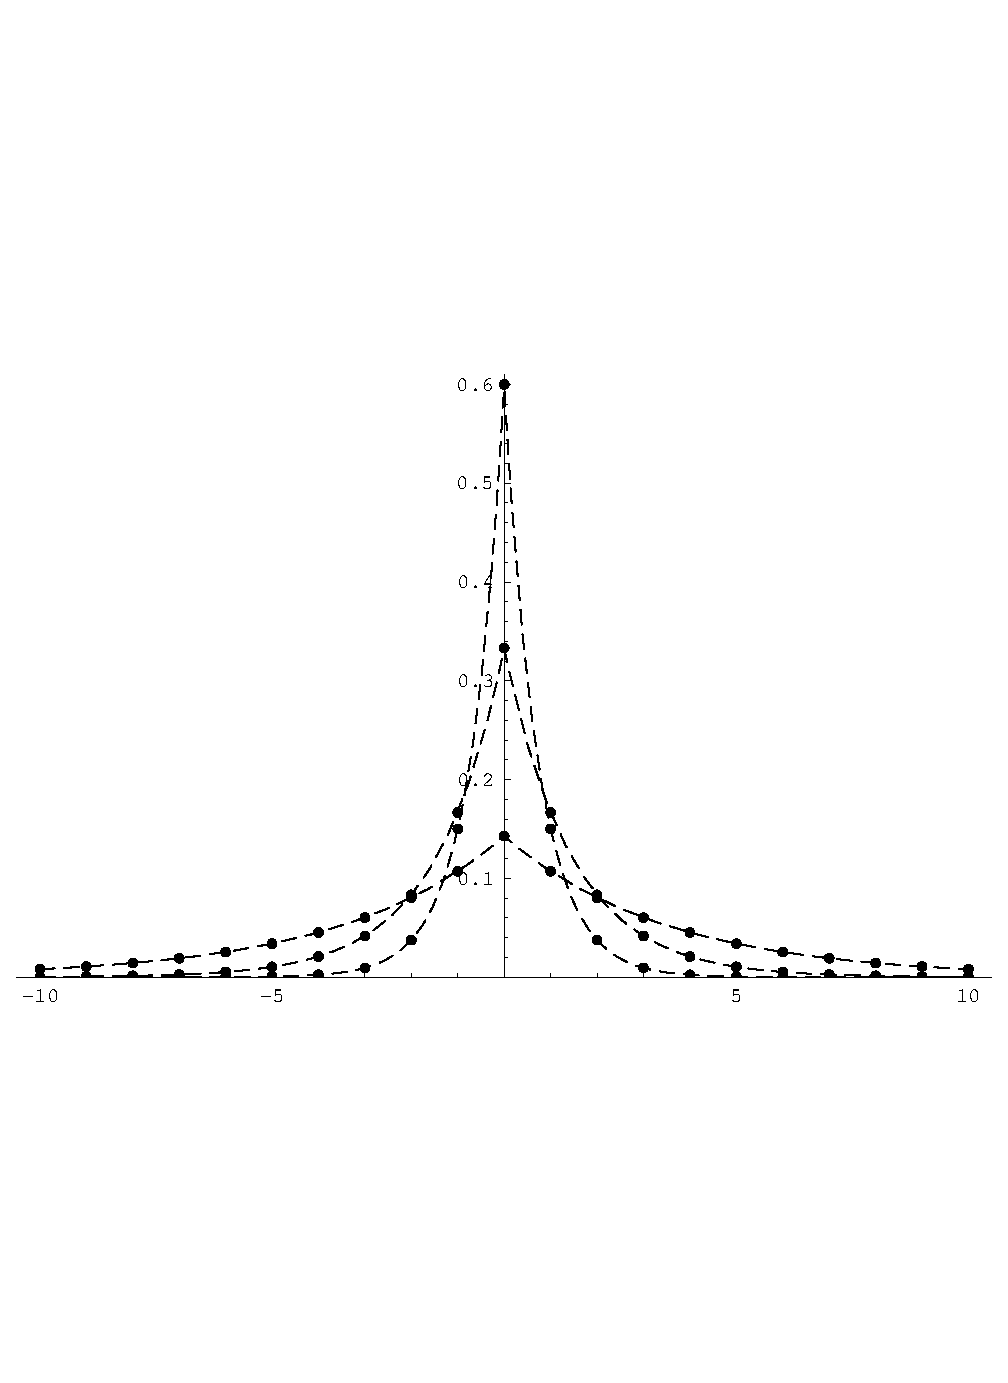
\includegraphics[width=\textwidth]{diffGeom.eps}
        \hfill
    }
    \vspace*{-30ex}
    \caption[Verteilung diskreter Zufallszahlen]{
        \label{verteilung}
        Verteilung der diskreten Zufallszahlen
    }
\end{figure}

\newpage
\subsubsection{Mutationsmethoden}

%---------------------------------------------------------------------------%
\setNormalInstance
\printMethodWithOneParam
{void}
{mutateDiffGeom}
{double}
{s}
{Schrittweite f\"ur die Verteilung der Zufallszahlen.}
{Zu jedem Allelwert des Chromosoms {\em this} wird ein Zufallswert addiert, wobei
 eine spezielle Verteilung von Zufallszahlen (s.o.) mit Schrittweite
 {\em s} benutzt wird.}
{Keiner.}
{Keine.}
%---------------------------------------------------------------------------%

\vspace{4ex}

%---------------------------------------------------------------------------%
\setNormalInstance
\setCorrectWidthThree{8pt}
\setParamOne{s}{const vector$<$ double $>$\&}{Vektor, der f\"ur jedes Allel von {\em this} eine
                            eigene Schrittweite f\"ur die 
                            Zufallszahlenverteilung angibt. {\em s} darf
                            maximal soviele Werte enthalten,
                            wie {\em this} Allele hat, sonst wird
die Methode mit einer Fehlermeldung abgebrochen.}
\setParamTwo{cycle}{bool}{Gibt f\"ur den Fall, da{\ss} {\em s} weniger Werte
                            enth\"alt, als {\em this} Allele hat an, ob der
                            Vektor mehrmals durchlaufen werden darf
                            oder nicht:\\
{\em true} - Der Vektor darf mehrmals durchlaufen werden,\\
{\em false} - Der Vektor darf nur einmal durchlaufen werden, dies entspricht
auch dem Default-Wert.}
\printMethodWithParamsSaved
{void}
{}
{mutateDiffGeom}
{Zu jedem Allelwert des Chromosoms {\em this} wird ein Zufallswert addiert, wobei
    eine spezielle Verteilung von Zufallszahlen (s.o.) mit einer
    Schrittweite benutzt wird, die f\"ur jedes Allel des Chromosoms
    separat im Vektor {\em s} angegeben wird. Da {\em s} weniger Werte enthalten kann,
    als {\em this} Allele hat, kann durch {\em cycle} angegeben werden, ob der
    Vektor mehrmals durchlaufen werden darf oder nicht.}
{}
\setCorrectWidthThree{4pt}
%---------------------------------------------------------------------------%

\newpage

%---------------------------------------------------------------------------%
\setNormalInstance
\setCorrectWidthThree{8pt}
\setParamOne{s}{const ChromosomeT$<$ double $>$\&}{Chromosom, das f\"ur jedes Allel von {\em this} eine
                            eigene Schrittweite f\"ur die 
                            Zufallszahlenverteilung angibt. {\em s} darf
                            maximal soviele Allele enthalten wie {\em this},
sonst wird die Methode mit einer Fehlermeldung abgebrochen.}
\setParamTwo{cycle}{bool}{Gibt f\"ur den Fall, da{\ss} {\em s} weniger 
                            Allele enth\"alt
                            als {\em this} an, ob das Chromosom {\em s}
                            mehrmals durchlaufen werden darf
                            oder nicht:\\
{\em true} - Das Chromosom darf mehrmals durchlaufen werden,\\
{\em false} - Das Chromosom darf nur einmal durchlaufen werden, dies
entspricht auch dem Default-Wert.}
\printMethodWithParamsSaved
{void}
{}
{mutateDiffGeom}
{Zu jedem Allelwert des Chromosoms {\em this} wird ein Zufallswert addiert, wobei
    eine spezielle Verteilung von Zufallszahlen (s.o.) mit einer
    Schrittweite benutzt wird, die f\"ur jedes Allel des Chromosoms {\em this}
    separat im Chromosom {\em s} angegeben wird. Da {\em s} weniger Allele als {\em this}  
    enthalten kann, kann durch {\em cycle} angegeben werden, ob das Chromosom
    {\em s} mehrmals durchlaufen werden darf oder nicht.}
{}
\setCorrectWidthThree{4pt}
%---------------------------------------------------------------------------%

\newpage

%---------------------------------------------------------------------------%
\setNormalInstance
\setCorrectWidthThree{8pt}
\setParamOne{s}{const Chromosome\&}{Chromosom, das f\"ur jedes Allel von {\em this} eine
                            eigene Schrittweite f\"ur die 
                            Zufallszahlenverteilung durch einen Wert
                            beliebigen Typs angibt. {\em s} darf
                            maximal soviele Allele enthalten wie {\em this},
sonst wird die Methode mit einer Fehlermeldung abgebrochen.}
\setParamTwo{cycle}{bool}{Gibt f\"ur den Fall, da{\ss} {\em s} weniger Allele 
                            enth\"alt
                            als {\em this} an, ob das Chromosom {\em s}
                            mehrmals durchlaufen werden darf
                            oder nicht:\\
{\em true} - Das Chromosom darf mehrmals durchlaufen werden,\\
{\em false} - Das Chromosom darf nur einmal durchlaufen werden, dies
entspricht auch dem Default-Wert.}
\printMethodWithParamsSaved
{void}
{}
{mutateDiffGeom}
{Zu jedem Allelwert des Chromosoms {\em this} wird ein Zufallswert addiert, wobei
    eine spezielle Verteilung von Zufallszahlen (s.o.) mit einer
    Schrittweite benutzt wird, die f\"ur jedes Allel des Chromosoms {\em this}
    separat im Chromosom {\em s} angegeben wird. {\em s} darf dabei im Gegensatz
    zur vorherigen Methode Werte beliebigen Typs beinhalten.
    Da {\em s} weniger Allele als {\em this} enthalten kann, kann durch {\em cycle} angegeben 
    werden, ob das Chromosom {\em s} mehrmals durchlaufen werden darf oder nicht.}
{}
\setCorrectWidthThree{4pt}
%---------------------------------------------------------------------------%

\newpage

\setNormalInstance

\noindent
\chapter{Klasse {\tt ChromosomeT$<$ char $>$}}
Diese Klasse enth\"alt Methoden und Datenstrukturen f\"ur die Arbeit
mit Chromosomen vom numerischen Typ {\tt character}.
Aufgebaut wird dabei auf den allgemeineren Klassen {\tt Chromosome} und
{\tt ChromosomeT\_num},
was zugleich hei{\ss}t, da{\ss} alle in den Referenzen zu diesen Klassen
genannten Methoden auch auf Chromosomen dieser spezielleren
{\tt character}-Klasse anwendbar sind.\\
Diese Methoden sind dann auch die einzigen f\"ur Chromosomen des
Typs {\tt char}, spezielle Methoden sind nicht vorgesehen.

\setNormalInstance

\noindent
\chapter{Klasse {\tt ChromosomeT$<$ bool $>$}}
Diese Klasse enth\"alt Methoden und Datenstrukturen f\"ur die Arbeit
mit Chromosomen vom numerischen bin\"aren Typ, der als
Wahrheitswert {\tt true} (gleich '1') bzw. {\tt false} (gleich '0')
interpretiert wird ({\tt boolean}).
Aufgebaut wird dabei auf den allgemeineren Klassen {\tt Chromosome}
und {\tt ChromosomeT\_num},
was zugleich hei{\ss}t, da{\ss} alle in den Referenzen zu diesen Klassen
genannten Methoden auch auf Chromosomen dieser spezielleren
{\tt boolean}-Klasse anwendbar sind.\\
In dieser Referenz werden die Methoden aufgef\"uhrt, die zus\"atzlich speziell
nur f\"ur Chromosomen des {\tt boolean}-Typs verwendbar sind. \\
Dabei wird in
den Methodenbeschreibungen das aktuelle Chromosom, d.h. jene Instanz der Klasse
{\tt ChromosomeT$<$ bool $>$}, die die aktuelle Methode aufgerufen hat, 
der Einfachheit halber als {\em this} bezeichnet, was der \cpp\ -internen 
Benennung entspricht.

\newpage
\section{Frei verf\"ugbare Methoden}
Diese Methoden d\"urfen von allen \cpp\ -Programmen benutzt werden, die
die Deklarationsdatei {\em ChromosomeT.h} und die Bibliothek {\em EA}
eingebunden haben.

\subsection{Initialisierungsmethoden}

%---------------------------------------------------------------------------%
\setNormalInstance
\printEmptyMethod
{initialize}
{Initialisiert die Allele des aktuellen Chromosoms per Zufall mit
    den Werten {\em true} oder {\em false}. Jede Belegung wird mit 
    gleicher Wahrscheinlichkeit gew\"ahlt.}
%---------------------------------------------------------------------------%

\newpage
\subsection{Kodierungsmethoden}

%---------------------------------------------------------------------------%
\setNormalInstance
\setCorrectWidthThree{8pt}
\setParamOne{val}{double}{Reelle Zahl, die kodiert werden soll.}
\setParamTwo{range}{const Interval\&}{Intervall aus dem die Zahl stammt.}
\setParamThree{nbits}{unsigned}{Anzahl der Bits, die zum Kodieren benutzt werden sollen.}
\setParamFour{useGray}{bool}{Gibt an, welche Kodierungsmethode angewandt werden soll:\\
 {\em true}\hspace{2pt} - Die Gray-Kodierung wird benutzt,\\
 {\em false} - Die Standard-Kodierung wird benutzt, dies ist auch der 
 Default-Wert.}
\printMethodWithParamsSaved
{void}
{}
{encode}
{Kodiert eine reelle Zahl {\em val} aus dem Intervall {\em range} in einen Bitstring
    der L\"ange {\em nbits}, der im Chromosom {\em this} abgelegt wird.
    Dabei gibt {\em useGray} an, ob zur Kodierung der Gray-Code
    benutzt werden soll oder nicht.}
{}
\setCorrectWidthThree{4pt}
%---------------------------------------------------------------------------%

\vspace{4ex}

%---------------------------------------------------------------------------%
\setNormalInstance
\setCorrectWidthThree{8pt}
\setParamOne{chrom}{const vector$<$ double $>$\&}{Vektor mit den zu kodierenden Zahlen.}
\setParamTwo{range}{const Interval\&}{Intervall, aus dem die Zahlen stammen.}
\setParamThree{nbits}{unsigned}{Anzahl der Bits, die zur Kodierung jeder
                              Zahl benutzt werden sollen.}
\setParamFour{useGray}{bool}{Gibt an, welche Methode zur Kodierung benutzt
                              werden soll:\\
{\em true}\hspace{2pt} - Die Gray-Kodierungsmethode wird
                                        benutzt,\\
                              {\em false} - Die Standard-Kodierungsmethode
                                        wird benutzt, dies ist auch der
                                        Default-Wert.}
\printMethodWithParamsSaved
{void}
{}
{encodeBinary}
{Kodiert die im Vektor {\em chrom} enthaltenen reellen Zahlen aus dem Intervall
    {\em range} in einen Bitstring, der im Chromosom {\em this} abgelegt wird. F\"ur
    die Kodierung jeder einzelnen Zahl werden {\em nbits} Bits benutzt und durch
    {\em useGray} wird die Kodierungsmethode angegeben.}
{}
\setCorrectWidthThree{4pt}
%---------------------------------------------------------------------------%

\newpage

%---------------------------------------------------------------------------%
\setNormalInstance
\setCorrectWidthThree{8pt}
\setParamOne{chrom}{const Chromosome\&}{Chromosom mit den zu kodierenden Zahlen.}
\setParamTwo{range}{const Interval\&}{Intervall, aus dem die Zahlen stammen.}
\setParamThree{nbits}{unsigned}{Anzahl der Bits, die zur Kodierung jeder
                              Zahl benutzt werden sollen.}
\setParamFour{useGray}{bool}{Gibt an, welche Methode zur Kodierung benutzt
                              werden soll:\\
                              {\em true}\hspace{2pt} - Die Gray-Kodierungsmethode wird
                                        benutzt,\\
                              {\em false} - Die Standard-Kodierungsmethode
                                        wird benutzt, dies ist auch der
                                        Default-Wert.}
\printMethodWithParamsSaved
{void}
{}
{encodeBinary}
{Kodiert die in den Allelen des Chromosoms {\em chrom} enthaltenen reellen Zahlen 
    aus dem Intervall {\em range} in einen Bitstring, der im Chromosom {\em this} abgelegt 
    wird. F\"ur die Kodierung jeder einzelnen Zahl werden {\em nbits} Bits benutzt und 
    durch {\em useGray} wird die Kodierungsmethode angegeben.}
{}
\setCorrectWidthThree{4pt}
%---------------------------------------------------------------------------%

\subsection{Dekodierungsmethoden}

%---------------------------------------------------------------------------%
\setConstInstance
\setCorrectWidthThree{8pt}
\setParamOne{range}{const Interval\&}{Intervall, aus dem die Zahl stammt.}
\setParamTwo{useGray}{bool}{Gibt die Methode an, die zur Kodierung der
                              Zahl benutzt wurde:\\
                              {\em true}\hspace{2pt} - Der Gray-Code wurde zur Kodierung
                                        benutzt,\\
                              {\em false} - Es wurde die Standardmethode zur
                                        Kodierung benutzt, dies ist auch
                                        der Default-Wert.}
\printMethodWithParamsSaved
{double}
{Die dekodierte reelle Zahl.}
{decode}
{Dekodiert eine im Chromosom als Bitstring kodierte reelle Zahl aus dem
    Intervall {\em range}.\\
    {\em useGray} gibt an, nach welcher Methode die Zahl
    kodiert wurde.}
{}
\setCorrectWidthThree{4pt}
%---------------------------------------------------------------------------%


\newpage 
\subsection{Mutationsmethoden}


%---------------------------------------------------------------------------%
\setNormalInstance
\printMethodWithOneParam
{void}
{flip}
{double}
{p}
{Wahrscheinlichkeit, mit der ein Allelwert invertiert 
                        wird.}
{Jedes Allel des aktuellen Chromosoms {\em this} wird mit einer Wahrscheinlichkeit
    von {\em p} invertiert, d.h. ein vorheriger Wert von {\em true} wird zu {\em false}
    und umgekehrt.}
{Keiner.}
{Keine.}
%---------------------------------------------------------------------------%

\vspace{4ex}

%---------------------------------------------------------------------------%
\setNormalInstance
\setCorrectWidthThree{8pt}
\setParamOne{p}{const vector$<$ double $>$\&}{Vektor mit Wahrscheinlichkeitswerten f\"ur
                            die entsprechenden Allele von this, invertiert
                            zu werden. {\em p} darf h\"ochstens soviele Werte
                            enthalten, wie {\em this} Allele hat, sonst
wird die Methode mit einer Fehlermeldung abgebrochen.}
\setParamTwo{cycle}{bool}{Gibt f\"ur den Fall, da{\ss} {\em p} weniger 
                            Wahrscheinlichkeitswerte enth\"alt, als {\em this} Allele
                            hat an, ob {\em p} mehrmals durchlaufen werden
                            darf:\\
                            {\em true}\hspace{2pt} - {\em p} darf mehrmals durchlaufen werden,\\
                            {\em false} - {\em p} darf nur einmal durchlaufen werden, dies ist auch der Default-Wert.}

\printMethodWithParamsSaved
{void}
{}
{flip}
{Jedes Allel des aktuellen Chromosoms {\em this} wird mit einer bestimmten
    Wahrscheinlichkeit invertiert, d.h. ein vorheriger Wert von {\em true} wird 
    zu {\em false} und umgekehrt. Die Werte von Vektor {\em p} geben f\"ur jedes
    entsprechende Allel von {\em this} die Wahrscheinlichkeit an, mit der es 
    invertiert wird. Da {\em p} weniger Wahrscheinlichkeitswerte enthalten kann,
    als {\em this} Allele hat, kann mittles {\em cycle} angegeben werden, ob 
    {\em p} mehrmals durchlaufen werden darf oder nicht.}
{}
\setCorrectWidthThree{4pt}
%---------------------------------------------------------------------------%

\newpage

%---------------------------------------------------------------------------%
\setNormalInstance
\setCorrectWidthThree{8pt}
\setParamOne{p}{const Chromosome\&}{Chromosom mit Wahrscheinlichkeitswerten f\"ur
                            die entsprechenden Allele von this, invertiert
                            zu werden. {\em p} darf h\"ochstens soviele Allele
                            enthalten, wie {\em this}, sonst
wird die Methode mit einer Fehlermeldung abgebrochen.}
\setParamTwo{cycle}{bool}{Gibt f\"ur den Fall, da{\ss} {\em p} weniger Allele als {\em this} 
                            enth\"alt an, ob {\em p} mehrmals durchlaufen
                            werden darf:\\
                            {\em true}\hspace{2pt} - {\em p} darf mehrmals durchlaufen werden,\\
                            {\em false} - {\em p} darf nur einmal durchlaufen werden, dies ist auch der Default-Wert.}

\printMethodWithParamsSaved
{void}
{}
{flip}
{Jedes Allel des aktuellen Chromosoms {\em this} wird mit einer bestimmten
    Wahrscheinlichkeit invertiert, d.h. ein vorheriger Wert von {\em true} wird 
    zu {\em false} und umgekehrt. Die Allelwerte von Chromosom {\em p} geben f\"ur jedes
    entsprechende Allel von {\em this} die Wahrscheinlichkeit an, mit der es 
    invertiert wird. Da {\em p} weniger Allele als {\em this} enthalten kann,
    kann mittles {\em cycle} angegeben werden, ob {\em p} mehrmals durchlaufen 
    werden darf oder nicht.}
{}
\setCorrectWidthThree{4pt}
%---------------------------------------------------------------------------%

\setNormalInstance

\noindent
\chapter{Klasse {\tt Individual}}
Die Klasse {\tt Individual} stellt Datenstrukturen und Methoden f\"ur 
Individuen einer Population bereit.\\
Ein Individuum besteht dabei aus einer bestimmten Anzahl von
Chromosomen beliebigen Typs (dem sogenannten {\em Genom}), wobei die 
Chromosomen eines Individuums durchaus unterschiedliche Typen besitzen 
k\"onnen. Intern wird ein
Individuum als ein Vektor von Zeigern auf Chromosomen verwaltet.\\
Im Folgenden wird das aktuelle Individuum, d.h. jene Instanz der Klasse
{\tt Individual}, die die aktuelle Methode aufgerufen hat, der Einfachheit 
halber als {\em this} bezeichnet, was der \cpp\ -internen Benennung
entspricht.

\section{Interne Variablen und Flags}
Die Klasse {\tt Individual} besitzt einige interne Variablen und Flags,
die f\"ur die Durchf\"uhrung verschiedener Methoden ben\"otigt werden.
Diese Daten k\"onnen nicht direkt vom Benutzer ver\"andert werden, jedoch
stellt die Klasse einige Methoden zur Ver\"anderung und zum Abruf der Werte
zur Verf\"ugung. Hier nun die Daten im einzelnen:\\

\subsection{Interne Variablen}
\begin{itemize}
\item {\em fitness} -
Ergebnis der Bewertung des Individuums; wird bei Initialisierung auf 
``0'' gesetzt.

\item {\em scaledFitness} -
Der von einer Bewertungsfunktion {\em f} erzeugte Wert wird mittels
einer Skalierungsfunktion auf einen positiven Fitne{\ss}-Wert abgebildet.
Die Summe der abgebildeten Fitne{\ss}-Werte aller Individuen aus der 
Population der Eltern mu{\ss} dabei zus\"atzlich ``1.0'' ergeben.\\
Diese normalisierten Werte werden skalierte Fitne{\ss}-Werte genannt und
bei der Initialisierung eines Individuums wird die ihm zugeh\"orige
skalierte Fitne{\ss} auf ``0'' gesetzt.

\item {\em age} -
Gibt das Alter des Individuums an; wird bei Initialisierung auf ``0''
gesetzt.

\item {\em selProb} - Die Selektionswahrscheinlichkeit des Individuums; wird 
bei Initialisierung auf ``0'' gesetzt.

\item {\em numCopies} -
Gibt an, wie oft das Individuum bei der letzten Selektion
reproduziert wurde und wird bei Initialisierung auf ``0'' gesetzt.

\end{itemize}

\newpage

\subsection{Interne Flags}
\begin{itemize}

\item {\em evalFlg} -
Gibt an, ob die Fitne{\ss} des Individuums bewertet werden
mu{\ss} oder nicht. Das Flag kann folgende Werte annehmen:
\begin{enumerate}
\item {\em true} - Das Individuum mu{\ss} bewertet werden.
\item {\em false} - Das Individuum braucht keine Bewertung. 
\end{enumerate}
Das Flag wird bei der Initialisierung auf ``false'' gesetzt.

\item {\em feasible} -
Gibt an, ob das Individuum eine m\"ogliche L\"osung 
des Optimierungsproblems darstellt oder nicht. Das Flag kann folgende
Werte annehmen:
\begin{enumerate}
\item {\em true} - Das Individuum stellt eine m\"ogliche Loesung dar.
\item {\em false} - Das Individuum bietet keine L\"osung.
\end{enumerate}
Das Flag wird bei der Initialisierung auf ``false'' gesetzt.

\item {\em elitist} -
Gibt an, ob das Individuum bei der letzten Selektion als 
Elitist ausgew\"ahlt wurde oder nicht. Das Flag kann folgende Werte
annehmen:
\begin{enumerate}
\item {\em true} - Das Individuum wurde als Elitist ausgew\"ahlt.
\item {\em false} - Das Individuum wurde nicht als Elitist ausgew\"ahlt.
\end{enumerate}
Das Flag wird bei der Initialisierung auf ``false'' gesetzt.

\end{itemize}

\section{Frei verf\"ugbare Methoden}
Diese Methoden d\"urfen von allen \cpp\ -Programmen benutzt werden, die
die Deklarationsdatei {\em Individual.h} und
die Bibliothek {\em EA} eingebunden haben.


\subsection{Konstruktoren}

%---------------------------------------------------------------------------%
\setNormalInstance
\printEmptyMethod
{Individual}
{Erzeugt ein leeres Individuum.}
%---------------------------------------------------------------------------%

\vspace{4ex}

%---------------------------------------------------------------------------%
\setNormalInstance
\printMethodWithOneParam
{explicit}
{Individual}
{unsigned}
{n}
{Anzahl der Chromosomen.}
{Erzeugt ein Individuum, welches aus {\em n} Chromosomen des
    Typs {\tt char} besteht.}
{Keiner.}
{{\em explicit} = Implizite Aufrufe des Konstruktors bei Anweisungen
 der Form {\tt Individual} {\em ind} = $<$Wert$>$ sind nicht m\"oglich.}
%---------------------------------------------------------------------------%

\newpage

%---------------------------------------------------------------------------%
\setNormalInstance
\setCorrectWidthThree{8pt}
\setParamOne{n}{unsigned}{Anzahl der Klone.}
\setParamTwo{chrom}{const Chromosome\&}{Zu klonendes Chromosom.}
\printMethodWithParamsSaved
{}
{}
{Individual}
{Erzeugt ein Individuum, welches aus {\em n} Klonen des 
                    Chromosoms
    {\em chrom} besteht.}
{}
\setCorrectWidthThree{4pt}
%---------------------------------------------------------------------------%

\vspace{4ex}

%---------------------------------------------------------------------------%
\setNormalInstance
\printMethodWithOneParam
{}
{Individual}
{const Chromosome\&}
{chrom0}
{Chromosom, dessen Klon das Individuum bildet.}
{Erzeugt ein Individuum, welches aus dem Chromosom
    {\em chrom0} besteht.}
{Keiner.}
{Keine.}
%---------------------------------------------------------------------------%

\vspace{4ex}

%---------------------------------------------------------------------------%
\setNormalInstance
\setCorrectWidthThree{8pt}
\setParamOne{chrom0}{const Chromosome\&}{Erstes Chromosomen, dessen Klon einen
                             Teil von {\em this} ausmacht.}
\setParamTwo{chrom1}{const Chromosome\&}{Zweites Chromosomen, dessen Klon einen
                             Teil von {\em this} ausmacht.}
\printMethodWithParamsSaved
{}
{}
{Individual}
{Erzeugt ein Individuum, welches aus den Chromosomen
    {\em chrom0} und {\em chrom1} besteht.}
{}
\setCorrectWidthThree{4pt}
%---------------------------------------------------------------------------%

\newpage

%---------------------------------------------------------------------------%
\setNormalInstance
\printMethodWithOneParam
{}
{Individual}
{const Chromosome\&}
{chrom0 .. chrom2}
{Chromosomen, deren Klone das Individuum {\em this} bilden.}
{Erzeugt ein Individuum, welches aus den Chromosomen
 {\em chrom0} bis {\em chrom2} besteht.}
{Keiner.}
{Keine.}
%---------------------------------------------------------------------------%

\vspace{4ex}

%---------------------------------------------------------------------------%
\setNormalInstance
\printMethodWithOneParam
{}
{Individual}
{const Chromosome\&}
{chrom0 .. chrom3}
{Chromosomen, deren Klone das Individuum {\em this} bilden.}
{Erzeugt ein Individuum, welches aus den Chromosomen
 {\em chrom0} bis {\em chrom3} besteht.}
{Keiner.}
{Keine.}
%---------------------------------------------------------------------------%

\vspace{4ex}

%---------------------------------------------------------------------------%
\setNormalInstance
\printMethodWithOneParam
{}
{Individual}
{const Chromosome\&}
{chrom0 .. chrom4}
{Chromosomen, deren Klone das Individuum {\em this} bilden.}
{Erzeugt ein Individuum, welches aus den Chromosomen
 {\em chrom0} bis {\em chrom4} besteht.}
{Keiner.}
{Keine.}
%---------------------------------------------------------------------------%

\newpage

%---------------------------------------------------------------------------%
\setNormalInstance
\printMethodWithOneParam
{}
{Individual}
{const Chromosome\&}
{chrom0 .. chrom5}
{Chromosomen, deren Klone das Individuum {\em this} bilden.}
{Erzeugt ein Individuum, welches aus den Chromosomen
 {\em chrom0} bis {\em chrom5} besteht.}
{Keiner.}
{Keine.}
%---------------------------------------------------------------------------%

\vspace{4ex}

%---------------------------------------------------------------------------%
\setNormalInstance
\printMethodWithOneParam
{}
{Individual}
{const Chromosome\&}
{chrom0 .. chrom6}
{Chromosomen, deren Klone das Individuum {\em this} bilden.}
{Erzeugt ein Individuum, welches aus den Chromosomen
 {\em chrom0} bis {\em chrom6} besteht.}
{Keiner.}
{Keine.}
%---------------------------------------------------------------------------%

\vspace{4ex}

%---------------------------------------------------------------------------%
\setNormalInstance
\printMethodWithOneParam
{}
{Individual}
{const Chromosome\&}
{chrom0 .. chrom7}
{Chromosomen, deren Klone das Individuum {\em this} bilden.}
{Erzeugt ein Individuum, welches aus den Chromosomen
 {\em chrom0} bis {\em chrom7} besteht.}
{Keiner.}
{Keine.}
%---------------------------------------------------------------------------%

\newpage

%---------------------------------------------------------------------------%
\setNormalInstance
\printMethodWithOneParam
{}
{Individual}
{const vector$<$ Chromosome* $>$\&}
{chrom}
{Vektor mit Chromosomen, deren Klone das
                            Individuum bilden.}
{Erzeugt ein Individuum, welches aus den Chromosomen
    besteht, die in dem Vektor {\em chrom} abgelegt sind.}
{Keiner.}
{Keine.}
%---------------------------------------------------------------------------%

\vspace{4ex}

%---------------------------------------------------------------------------%
\setNormalInstance
\printMethodWithOneParam
{}
{Individual}
{const Individual\&}
{indiv}
{Individuum, dessen Kopie das neue Individuum
                            bildet.}
{Erzeugt ein Individuum, welches eine Kopie des
    \"ubergebenen Individuums {\em indiv} darstellt. Auch die Belegung der
    internen Klassenvariablen wird von {\em indiv} \"ubernommen.}
{Keiner.}
{Keine.}
%---------------------------------------------------------------------------%

\subsection{Destruktor}

%---------------------------------------------------------------------------%
\printEmptyMethodReturnSpecial
{virtual}
{$\sim$Individual}
{L\"oscht alle im Individuum vorhandenen Chromosomen und zerst\"ort dann das 
 Individuum selbst.}
{Keiner.}
{Der Destruktor ist virtuell, die Funktionalit\"at kann von erbenden 
 Nachfolgeklassen benutzt und erweitert werden. Der Destruktor sollte nicht 
 direkt aufgerufen werden.}
%---------------------------------------------------------------------------%

\newpage

\subsection{Operatoren}

\subsubsection{Zuweisungsoperator}

%---------------------------------------------------------------------------%
\setNormalInstance
\printMethodWithOneParam
{Individual\&}
{operator =}
{const Individual\&}
{indiv}
{Individuum, welches dem Individuum {\em this} zugewiesen wird.}
{Weist dem aktuellen Individuum {\em this}
    das Individuum {\em indiv} (d.h. die in {\em indiv} enthaltenen Chromosomen
    und die in {\em indiv} vorhandene Belegung der internen Klassenvariablen)
    zu.}
{Das Individuum {\em this} mit den neuen Werten.}
{Keine.}
%---------------------------------------------------------------------------%

\subsubsection{Vergleichsoperatoren}

%---------------------------------------------------------------------------%
\setConstInstance
\printMethodWithOneParam
{bool}
{operator ==}
{const Individual\&}
{ind}
{Individuum, welches mit {\em this} verglichen wird.}
{Gibt an, ob das aktuelle Individuum {\em this}
    und das Individuum {\em ind} gleich sind. Die Individuen sind gleich, 
    wenn sie dieselbe Zahl von Chromosomen enthalten, alle Chromosomen
    von {\em this} gleich den entsprechenden Chromosomen von {\em ind}
    sind und ihre internen Variablen dieselben
    Werte aufweisen.}
{
 {\em true}  - Beide Individuen sind gleich,\\
 {\em false} - Die Individuen sind nicht gleich.}
{Keine.}
%---------------------------------------------------------------------------%

\vspace{4ex}

%---------------------------------------------------------------------------%
\setConstInstance
\printMethodWithOneParam
{bool}
{operator $<$}
{const Individual\&}
{ind}
{Individuum, das mit {\em this} verglichen wird.}    
{Gibt an, ob das aktuelle Individuum {\em this}
    kleiner als das Individuum {\em ind} ist. Dies ist der Fall, wenn 
    {\em this} weniger Chromosomen enth\"alt als {\em ind} bzw. bei
    gleicher Chromosomenzahl dann, wenn mindestens ein Chromosom
    von {\em this} kleiner ist als das entsprechende Chromosom
    von {\em ind}.}
{
 {\em true}  - {\em this} ist kleiner als {\em ind},\\
 {\em false} - {\em this} ist gr\"o{\ss}er oder gleich {\em ind}.}
{Keine.}
%---------------------------------------------------------------------------%

\newpage

%---------------------------------------------------------------------------%
\setConstInstance
\printMethodWithOneParam
{bool}
{operator $>$}
{const Individual\&}
{ind}
{Individuum, das mit {\em this} verglichen wird.}    
{Gibt an, ob das aktuelle Individuum {\em this}
    gr\"o{\ss}er als das Individuum {\em ind} ist. Dies ist der Fall, wenn 
    {\em this} mehr Chromosomen enth\"alt als {\em ind} bzw. bei
    gleicher Chromosomenzahl dann, wenn mindestens ein Chromosom
    von {\em this} gr\"o{\ss}er ist als das entsprechende Chromosom
    von {\em ind}.}
{
 {\em true}  - {\em this} ist gr\"o{\ss}er als {\em ind},\\
 {\em false} - {\em this} ist kleiner oder gleich {\em ind}.}
{Keine.}
%---------------------------------------------------------------------------%

\vspace{4ex}

%---------------------------------------------------------------------------%
\setConstInstance
\printMethodWithOneParam
{bool}
{operator $<=$}
{const Individual\&}
{ind}
{Individuum, das mit {\em this} verglichen wird.}    
{Gibt an, ob das aktuelle Individuum {\em this}
    kleiner oder gleich dem Individuum {\em ind} ist. Dies ist der Fall,    
    wenn {\em this} genauso viel Chromosomen oder weniger Chromosomen 
    enth\"alt 
    wie {\em ind} und jedes Chromosom von {\em this} kleiner oder
    gleich dem entsprechenden Chromosom von {\em ind} ist.}
{
 {\em true}  - {\em this} ist kleiner oder gleich {\em ind},\\
 {\em false} - {\em this} ist gr\"o{\ss}er als {\em ind}.}
{Keine.}
%---------------------------------------------------------------------------%

\vspace{4ex}

%---------------------------------------------------------------------------%
\setConstInstance
\printMethodWithOneParam
{bool}
{operator $>=$}
{const Individual\&}
{ind}
{Individuum, das mit {\em this} verglichen wird.}    
{Gibt an, ob das aktuelle Individuum {\em this}
    gr\"o{\ss}er oder gleich dem Individuum {\em ind} ist. Dies ist der Fall,    wenn {\em this} genauso viel Chromosomen oder mehr Chromosomen enth\"alt 
    wie {\em ind} und jedes Chromosom von {\em this} gr\"o{\ss}er oder
    gleich dem entsprechenden Chromosom von {\em ind} ist.}
{
 {\em true}  - {\em this} ist gr\"o{\ss}er oder gleich {\em ind},\\
 {\em false} - {\em this} ist kleiner als {\em ind}.}
{Keine.}
%---------------------------------------------------------------------------%

\newpage

%---------------------------------------------------------------------------%
\setConstInstance
\printMethodWithOneParam
{bool}
{operator $!=$}
{const Individual\&}
{ind}
{Individuum, das mit {\em this} verglichen wird.}    
{Gibt an, ob das aktuelle Individuum {\em this}
    ungleich dem Individuum {\em ind} ist. Dies ist der Fall,    
    wenn {\em this} und {\em ind} unterschiedlich viele Chromosomen haben,
    bzw. bei gleicher Chromosomenzahl dann, wenn mindestens ein Chromosom 
    von {\em this} nicht mit dem entsprechenden Chromosom von {\em ind}
    \"ubereinstimmt.}
{
 {\em true}  - {\em this} ist ungleich {\em ind},\\
 {\em false} - {\em this} und {\em ind} sind gleich.}
{Keine.}
%---------------------------------------------------------------------------%

\subsubsection{Operatoren zum Zugriff auf ein einzelnes Chromosom}

%---------------------------------------------------------------------------%
\setNormalInstance
\printMethodWithOneParam
{Chromosome\&}
{operator [\ ]}
{unsigned}
{i}
{Index des zur\"uckzugebenden Chromosoms. {\em i} mu{\ss}
                        kleiner als die Anzahl der im Individuum
                        enthaltenen Chromosomen sein, sonst wird die
Methode mit einer Fehlermeldung abgebrochen.}
{Gibt Chromosom Nummer {\em i} des Individuums zur\"uck.}
{Chromosom Nummer {\em i} des Individuums.}
{Keine.}
%---------------------------------------------------------------------------%

\newpage

\subsection{Informationsmethoden}

%---------------------------------------------------------------------------%
\setConstInstance
\printEmptyMethodReturn
{unsigned}
{size}
{Gibt die Anzahl der im Individuum enthaltenen Chromosomen zur\"uck.}
{Anzahl der Chromosomen.}
%---------------------------------------------------------------------------%

\vspace{4ex}

%---------------------------------------------------------------------------%
\setConstInstance
\printEmptyMethodReturn
{unsigned}
{totalSize}
{Gibt die Gesamtzahl der Allele der im Individuum gespeicherten Chromsomen
    zur\"uck.}
{Gesamtzahl der Allele.}
%---------------------------------------------------------------------------%

\vspace{4ex}

%---------------------------------------------------------------------------%
\setConstInstance
\printEmptyMethodReturn
{double}
{fitnessValue}
{Gibt den Fitne{\ss}-Wert des Individuums zur\"uck.}
{Fitne{\ss}-Wert des Individuums.}
%---------------------------------------------------------------------------%

\vspace{4ex}

%---------------------------------------------------------------------------%
\setConstInstance
\printEmptyMethodReturn
{unsigned}
{getAge}
{Gibt das Alter des Individuums zur\"uck.}
{Alter des Individuums.}
%---------------------------------------------------------------------------%

\newpage

%---------------------------------------------------------------------------%
\setConstInstance
\printEmptyMethodReturn
{bool}
{needEvaluation}
{Gibt an, ob das Individuum bewertet werden mu{\ss}.}
{Status von {\em evalFlg}:\\
 {\em true} - Eine Bewertung des Individuums ist n\"otig,\\
 {\em false} - Das Individuum braucht nicht bewertet zu werden.}
%---------------------------------------------------------------------------%

\vspace{4ex}

%---------------------------------------------------------------------------%
\setConstInstance
\printEmptyMethodReturn
{double}
{selectionProbability}
{Gibt die Selektionswahrscheinlichkeit des Individuums zur\"uck.}
{Selektionswahrscheinlichkeit des Individuums.}
%---------------------------------------------------------------------------%

\vspace{4ex}

%---------------------------------------------------------------------------%
\setConstInstance
\printEmptyMethodReturn
{bool}
{isFeasible}
{Gibt an, ob das Individuum eine m\"ogliche L\"osung darstellt.}
{Status des {\em feasible}-Flags:\\
 {\em true} - Das Individuum stellt eine m\"ogliche L\"osung dar,\\
 {\em false} - Das Individuum stellt keine m\"ogliche L\"osung dar.}
%---------------------------------------------------------------------------%

\vspace{4ex}

%---------------------------------------------------------------------------%
\setConstInstance
\printEmptyMethodReturn
{unsigned}
{numberOfCopies}
{Gibt an, wie oft das Individuum bei der letzten Selektion
    reproduziert wurde.}
{Anzahl der Reproduktionen des Individuums.}
%---------------------------------------------------------------------------%

\newpage

%---------------------------------------------------------------------------%
\setConstInstance
\printEmptyMethodReturn
{bool}
{isElitist}
{Gibt an, ob das Individuum bei der letzten Selektion als Elitist
    ausgew\"ahlt wurde.}
{Status des {\em elitist}-Flags:\\
 {\em true} - Das Individuum wurde als Elitist ausgew\"ahlt,\\
 {\em false} - Das Individuum wurde nicht als Elitist ausgew\"ahlt.}
%---------------------------------------------------------------------------%

\subsection{Methoden zur Ver\"anderung interner Variablen und Flags}

%---------------------------------------------------------------------------%
\setNormalInstance
\printMethodWithOneParam
{void}
{setFitness}
{double}
{fit}
{Neuer Wert f\"ur die normale und skalierte Fitne{\ss}
                          des Individuums.}
{Setzt den Fitne{\ss}-Wert und die skalierte Fitne{\ss} des Individuums
    auf den Wert {\em fit}.}
{Keiner.}
{Keine.}
%---------------------------------------------------------------------------%

\vspace{4ex}

%---------------------------------------------------------------------------%
\setNormalInstance
\printMethodWithOneParam
{void}
{setAge}
{unsigned}
{a}
{Neues Alter des Individuums, per Default auf ``0'' gesetzt.}
{Setzt das Alter des Individuums auf den neuen Wert {\em a}.}
{Keiner.}
{Keine.}
%---------------------------------------------------------------------------%

\vspace{4ex}

%---------------------------------------------------------------------------%
\setNormalInstance
\printEmptyMethod
{incAge}
{Erh\"oht das Alter des Individuums um den Wert eins.}
%---------------------------------------------------------------------------%

\newpage

%---------------------------------------------------------------------------%
\setNormalInstance
\printEmptyMethod
{setEvaluationFlag}
{Setzt {\em evalFlg} auf ``true''.}
%---------------------------------------------------------------------------%

\vspace{4ex}

%---------------------------------------------------------------------------%
\setNormalInstance
\printEmptyMethod
{clearEvaluationFlag}
{Setzt {\em evalFlg} auf ``false''.}
%---------------------------------------------------------------------------%

\vspace{4ex}

%---------------------------------------------------------------------------%
\setNormalInstance
\printMethodWithOneParam
{void}
{setFeasible}
{bool}
{f}
{Neuer Wert des {\em feasible}-Flags:\\
{\em true} - Das Individuum stellt eine m\"ogliche L\"osung dar,\\
{\em false} - Das Individuum stellt keine m\"ogliche L\"osung dar.}
{Setzt das {\em feasible}-Flag auf den neuen Wert {\em f}.}
{Keiner.}
{Keine.}
%---------------------------------------------------------------------------%

\vspace{4ex}

%---------------------------------------------------------------------------%
\setNormalInstance
\printMethodWithOneParam
{void}
{setSelectionProbability}
{double}
{ps}
{Neue Selektionswahrscheinlichkeit f\"ur das 
                         Individuum.}
{Setzt die Selektionswahrscheinlichkeit des Individuums auf den Wert {\em ps}.}
{Keiner.}
{Keine.}
%---------------------------------------------------------------------------%

\newpage

\subsection{Strukturver\"anderungsmethoden}

%---------------------------------------------------------------------------%
\setNormalInstance
\setCorrectWidthThree{8pt}
\setParamOne{i}{unsigned}{Nummer des Chromosoms, welches ersetzt werden 
                            soll.
                            {\em i} mu{\ss} kleiner als die Anzahl der im Individuum
                            vorhandenen Chromosomen sein, sonst wird die
Methode mit einer Fehlermeldung abgebrochen.}
\setParamTwo{chrom}{const Chromosome\&}{Chromosom, dessen Klon das alte 
Chromosom von {\em this} ersetzt.}
\printMethodWithParamsSaved
{void}
{}
{replace}
{Ersetzt Chromosom Nummer {\em i} des Individuums durch das Chromosom 
    {\em chrom}.}
{}
\setCorrectWidthThree{4pt}
%---------------------------------------------------------------------------%

\vspace{4ex}

%---------------------------------------------------------------------------%
\setNormalInstance
\setCorrectWidthThree{8pt}
\setParamOne{i}{unsigned}{Position, an der das 
                            neue Chromosom {\em chrom} in {\em this} eingef\"ugt wird.
                            {\em i} mu{\ss} kleiner oder gleich der Anzahl der im 
                            Individuum vorhandenen Chromosomen sein, sonst
wird die Methode mit einer Fehlermeldung abgebrochen.}
\setParamTwo{chrom}{const Chromosome\&}{Chromosom, das in {\em this}
eingef\"ugt werden soll.}
\printMethodWithParamsSaved
{void}
{}
{insert}
{F\"ugt das Chromosom {\em chrom} als neues Chromosom Nummer {\em i} in das Individuum {\em this}
    ein.}
{}
\setCorrectWidthThree{4pt}
%---------------------------------------------------------------------------%

\vspace{4ex}

%---------------------------------------------------------------------------%
\setNormalInstance
\printMethodWithOneParam
{void}
{append}
{const Chromosome\&}
{chrom}
{Chromosom, das am Ende des Individuums
                            angeh\"angt wird.}
{H\"angt das Chromosom {\em chrom} am Ende des Individuums an.}
{Keiner.}
{Keine.}
%---------------------------------------------------------------------------%

\newpage

%---------------------------------------------------------------------------%
\setNormalInstance
\printMethodWithOneParam
{void}
{remove}
{unsigned}
{i}
{Nummer des Chromosoms, welches gel\"oscht werden soll.
                        {\em i} mu{\ss} kleiner als die Anzahl der Chromosomen des
                        Individuums sein, sonst wird die Methode mit einer
Fehlermeldung abgebrochen.}
{L\"oscht Chromosom Nummer {\em i} aus dem Individuum.}
{Keiner.}
{Keine.}
%---------------------------------------------------------------------------%

\vspace{4ex}

%---------------------------------------------------------------------------%
\setNormalInstance
\setCorrectWidthThree{8pt}
\setParamOne{from}{unsigned}{Position des ersten Chromosoms, welches gel\"oscht 
                           werden soll. {\em from} mu{\ss} kleiner als die Anzahl
                           der im Individuum vorhandenen Chromosomen und
                           kleiner oder gleich {\em to} sein, sonst
wird die Methode mit einer Fehlermeldung abgebrochen.}
\setParamTwo{to}{unsigned}{Position des letzten Chromosoms, welches gel\"oscht
                           werden soll. {\em to} mu{\ss} kleiner als die Anzahl
                           der im Individuum vorhandenen Chromosomen und
                           gr\"o{\ss}er oder gleich {\em from} sein, sonst
wird die Methode mit einer Fehlermeldung abgebrochen.}
\printMethodWithParamsSaved
{void}
{}
{remove}
{L\"oscht die Chromosomen an den Positionen {\em from} bis {\em to} aus dem Individuum {\em this}.}
{}
\setCorrectWidthThree{4pt}
%---------------------------------------------------------------------------%

\newpage

\subsection{Ein-/Ausgabemethoden}

%---------------------------------------------------------------------------%
\setNormalInstance
\printMethodWithOneParam
{void}
{readFrom}
{istream\&}
{is}
{Eingabstrom, aus dem die Daten des Individuums gelesen
                         werden.}
{Ersetzt die Daten des aktuellen Individuums {\em this} durch die Daten, die
    aus dem Eingabstrom {\em is} gelesen werden. Der Eingabestrom mu{\ss} dabei
    folgende Datenkomponenten enthalten:\\
    ``{\tt Individual(}'',\\
    Gr\"o{\ss}e des Individuums,\\ 
    ``{\tt )}'', Newline-Zeichen,\\ 
    Fitne{\ss}-Wert des Individuums, Newline-Zeichen,\\
    skalierte Fitne{\ss} des Individuums, Newline-Zeichen,\\
    Wert von {\em evalFlg}, Newline-Zeichen,\\
    Wert des {\em feasible}-Flags, Newline-Zeichen,\\
    Selektionswahrscheinlichkeit des Individuums, Newline-Zeichen,\\
    Anzahl der Reproduktionen des Individuums, Newline-Zeichen,\\
    Wert des {\em elitist}-Flags, Newline-Zeichen,\\
    Alter des Individuums, Newline-Zeichen,\\
    Dann folgen je nach Gr\"o{\ss}e des Individuums die Daten f\"ur die 
    einzelnen Chromosomen in folgendem Format:\\
    ``{\tt ChromosomeT$<$}'',\\
    Typ des Chromosoms,\\ 
    ``{\tt $>$(}'',\\ 
    Anzahl der Chromosomenallele,\\
    ``{\tt )}'', Newline-Zeichen,\\
    Werte der einzelnen Allele, durch ein Leerzeichen oder einen
    Tabulatorvorsprung getrennt.}
{Keiner.}
{Keine.}
%---------------------------------------------------------------------------%

\vspace{4ex}

%---------------------------------------------------------------------------%
\setConstInstance
\printMethodWithOneParam
{void}
{writeTo}
{ostream\&}
{os}
{Strom, auf dem die Ausgabe erfolgen soll.}
{Gibt die Daten des aktuellen Individuums {\em this} inklusive aller 
 Allelwerte seiner Chromosomen auf dem Ausgabestrom {\em os} aus.}
{Keiner.}
{Keine.}
%---------------------------------------------------------------------------%

\setNormalInstance

\noindent
\chapter{Klasse {\tt Population}}
Die Klasse {\tt Population} stellt Datenstrukturen und Methoden f\"ur 
eine Population bereit, die aus Individuen besteht, die sich
wiederum aus Chromosomen zusammensetzen.\\
Intern wird eine
Population als ein Vektor von Zeigern auf Individuen verwaltet.\\
Im Folgenden wird die aktuelle Population, d.h. jene Instanz der Klasse
{\tt Population}, die die aktuelle Methode aufgerufen hat, der Einfachheit 
halber als {\em this} bezeichnet, was der \cpp\ -internen Benennung
entspricht.

\section{Interne Variablen und Flags}
Die Klasse {\tt Population} besitzt einige interne Variablen und Flags,
die f\"ur die Durch\-f\"uhr\-ung verschiedener Methoden ben\"otigt werden.
Diese Daten k\"onnen nicht direkt vom Benutzer ver\"andert werden, jedoch
stellt die Klasse einige Methoden zur Ver\"anderung und zum Abruf dieser Werte
zur Verf\"ugung. Hier nun die Daten im einzelnen:\\

\subsection{Interne Variablen}
\begin{itemize}

\item {\em index} -
Gibt den Index des Individuums mit dem besten Fitne{\ss}-Wert innerhalb der
Population an. Diese Variable wird nicht explizit initialisiert.

\end{itemize}


\subsection{Interne Flags}
\begin{itemize}

\item {\em subPop} -
Gibt an, ob es sich bei der Population um eine 
Subpopulation handelt oder nicht. Eine Subpopulation entsteht durch 
ausl\"oschende Selektion ({\em extincive selection}), bei der Individuen 
auch eine Selektionswahrscheinlichkeit von ``0'' zugewiesen werden kann. 
Das Flag kann folgende Werte annehmen:
\begin{enumerate}
\item {\em true} - Bei der aktuellen Population handelt es sich um
 eine Subpopulation.
\item {\em false} - Die aktuelle Population ist keine Subpopulation.
\end{enumerate}
Bei einer Initialisierung wird das Flag auf ``false'' gesetzt.

\newpage
\item {\em ascending} -
Die einzelnen Individuen einer Population k\"onnen nach ihren 
Fitne{\ss}werten geordnet werden. Das {\em ascending}-Flag bestimmt dabei die Art 
der Ordnung. 
Das Flag kann folgende Werte annehmen:
\begin{enumerate}
\item {\em true} - Die Individuen werden innerhalb der Population nach 
aufsteigenden Fitne{\ss}-Werten geordnet.
\item {\em false} - Die Individuen werden nach absteigender Fitne{\ss} 
 sortiert.
\end{enumerate}
Bei einer Initialisierung wird das Flag auf ``false'' gesetzt.

\item {\em spinOnce} -
Bei der Selektion von Individuen f\"ur eine
Reproduktion in der n\"achsten Generation einer Population wird oft die
sogenannte Rouletterad-Selektion verwendet ({\em Roulette-Wheel-Selection}).
Das {\em spinOnce}-Flag gibt dabei an, wie oft sich das
``Rad'' bei der Selektion dreht. Das Flag kann folgende Werte annehmen:
\begin{enumerate}
\item {\em true} - Das Rad dreht sich nur einmal.
\item {\em false} - Das Rad dreht sich mehrmals.
\end{enumerate}
Bei einer Initialisierung wird das Flag auf ``true'' gesetzt.

\end{itemize}
\newpage
\section{Frei verf\"ugbare Methoden}
Diese Methoden d\"urfen von allen \cpp\ -Programmen benutzt werden, die
die Deklarationsdatei {\em Population.h} und
die Bibliothek {\em EA} eingebunden haben.


\subsection{Konstruktoren}

%---------------------------------------------------------------------------%
\setNormalInstance
\printEmptyMethod
{Population}
{Erzeugt eine leere Population.}
%---------------------------------------------------------------------------%

\vspace{4ex}

%---------------------------------------------------------------------------%
\setNormalInstance
\printMethodWithOneParam
{explicit}
{Population}
{unsigned}
{n}
{Anzahl der Individuen in der neuen Population.}
{Erzeugt eine neue Population und reserviert Platz
    f\"ur {\em n} Individuen unbestimmten Typs.}
{Keiner.}
{{\em explicit} = Implizite Aufrufe des Konstruktors bei Anweisungen
                    der Form Population {\em pop} = $<$Wert$>$ sind nicht m\"oglich.}
%---------------------------------------------------------------------------%

\newpage

%---------------------------------------------------------------------------%
\setNormalInstance
\printMethodWithOneParam
{}
{Population}
{const Individual\&}
{indiv}
{Individuum, das die neue Population bildet.}
{Erzeugt eine neue Population, die aus dem Individuum
    {\em indiv} besteht.}
{Keiner.}
{Keine.}
%---------------------------------------------------------------------------%

\vspace{4ex}

%---------------------------------------------------------------------------%
\setNormalInstance
\setCorrectWidthThree{8pt}
\setParamOne{n}{unsigned}{Anzahl der Kopien von {\em indiv}, die die Population bilden.}
\setParamTwo{indiv}{const Individual\&}{Individuum, dessen Kopien die neue Population
                            bilden.}
\printMethodWithParamsSaved
{}
{}
{Population}
{Erzeugt eine neue Population, die aus {\em n} Kopien des
    Individuums {\em indiv} besteht.}
{}
\setCorrectWidthThree{4pt}
%---------------------------------------------------------------------------%

\vspace{4ex}

%---------------------------------------------------------------------------%
\setNormalInstance
\setCorrectWidthThree{8pt}
\setParamOne{n}{unsigned}{Anzahl der Individuen, aus denen die neue
Population bestehen soll.}
\setParamTwo{chrom0}{const Chromosome\&}{Chromosom, dessen Klon je ein Individuum 
                             der Population bildet.}
\printMethodWithParamsSaved
{}
{}
{Population}
{Erzeugt eine neue Population, die aus {\em n} Individuen
    besteht, die wiederum je aus einem Klon des Chromosoms {\em chrom0}
    bestehen.}
{}
\setCorrectWidthThree{4pt}
%---------------------------------------------------------------------------%

\newpage

%---------------------------------------------------------------------------%
\setNormalInstance
\setCorrectWidthThree{8pt}
\setParamOne{n}{unsigned}{Anzahl der Individuen, aus denen die 
                                       neue Population bestehen soll.}
\setParamTwo{chrom0 .. chrom1}{const Chromosome\&}{Chromosomen, deren Klone je ein 
                                       Individuum der Population bilden.}
\printMethodWithParamsSaved
{}
{}
{Population}
{Erzeugt eine neue Population, die aus {\em n} Individuen
    besteht, die wiederum je aus Klonen der Chromosomen {\em chrom0} und {\em chrom1}
    bestehen.}
{}
\setCorrectWidthThree{4pt}
%---------------------------------------------------------------------------%

\vspace{4ex}

%---------------------------------------------------------------------------%
\setNormalInstance
\setCorrectWidthThree{8pt}
\setParamOne{n}{unsigned}{Anzahl der Individuen, aus denen die 
                                       neue Population bestehen soll.}
\setParamTwo{chrom0 .. chrom2}{const Chromosome\&}{Chromosomen, deren Klone je ein 
                                       Individuum der Population bilden.}
\printMethodWithParamsSaved
{}
{}
{Population}
{Erzeugt eine neue Population, die aus {\em n} Individuen
    besteht, die wiederum je aus Klonen der Chromosomen {\em chrom0} bis {\em chrom2}
    bestehen.}
{}
\setCorrectWidthThree{4pt}
%---------------------------------------------------------------------------%

\vspace{4ex}

%---------------------------------------------------------------------------%
\setNormalInstance
\setCorrectWidthThree{8pt}
\setParamOne{n}{unsigned}{Anzahl der Individuen, aus denen die 
                                       neue Population bestehen soll.}
\setParamTwo{chrom0 .. chrom3}{const Chromosome\&}{Chromosomen, deren Klone je ein 
                                       Individuum der Population bilden.}
\printMethodWithParamsSaved
{}
{}
{Population}
{Erzeugt eine neue Population, die aus {\em n} Individuen
    besteht, die wiederum je aus Klonen der Chromosomen {\em chrom0} bis {\em chrom3}
    bestehen.}
{}
\setCorrectWidthThree{4pt}
%---------------------------------------------------------------------------%

\newpage

%---------------------------------------------------------------------------%
\setNormalInstance
\setCorrectWidthThree{8pt}
\setParamOne{n}{unsigned}{Anzahl der Individuen, aus denen die 
                                       neue Population bestehen soll.}
\setParamTwo{chrom0 .. chrom4}{const Chromosome\&}{Chromosomen, deren Klone je ein 
                                       Individuum der Population bilden.}
\printMethodWithParamsSaved
{}
{}
{Population}
{Erzeugt eine neue Population, die aus {\em n} Individuen
    besteht, die wiederum je aus Klonen der Chromosomen {\em chrom0} bis {\em chrom4}
    bestehen.}
{}
\setCorrectWidthThree{4pt}
%---------------------------------------------------------------------------%

\vspace{4ex}

%---------------------------------------------------------------------------%
\setNormalInstance
\setCorrectWidthThree{8pt}
\setParamOne{n}{unsigned}{Anzahl der Individuen, aus denen die 
                                       neue Population bestehen soll.}
\setParamTwo{chrom0 .. chrom5}{const Chromosome\&}{Chromosomen, deren Klone je ein 
                                       Individuum der Population bilden.}
\printMethodWithParamsSaved
{}
{}
{Population}
{Erzeugt eine neue Population, die aus {\em n} Individuen
    besteht, die wiederum je aus Klonen der Chromosomen {\em chrom0} bis {\em chrom5}
    bestehen.}
{}
\setCorrectWidthThree{4pt}
%---------------------------------------------------------------------------%

\vspace{4ex}

%---------------------------------------------------------------------------%
\setNormalInstance
\setCorrectWidthThree{8pt}
\setParamOne{n}{unsigned}{Anzahl der Individuen, aus denen die 
                                       neue Population bestehen soll.}
\setParamTwo{chrom0 .. chrom6}{const Chromosome\&}{Chromosomen, deren Klone je ein 
                                       Individuum der Population bilden.}
\printMethodWithParamsSaved
{}
{}
{Population}
{Erzeugt eine neue Population, die aus {\em n} Individuen
    besteht, die wiederum je aus Klonen der Chromosomen {\em chrom0} bis {\em chrom6}
    bestehen.}
{}
\setCorrectWidthThree{4pt}
%---------------------------------------------------------------------------%

\newpage

%---------------------------------------------------------------------------%
\setNormalInstance
\setCorrectWidthThree{8pt}
\setParamOne{n}{unsigned}{Anzahl der Individuen, aus denen die 
                                       neue Population bestehen soll.}
\setParamTwo{chrom0 .. chrom7}{const Chromosome\&}{Chromosomen, deren Klone 
je ein Individuum der Population bilden.}
\printMethodWithParamsSaved
{}
{}
{Population}
{Erzeugt eine neue Population, die aus {\em n} Individuen
    besteht, die wiederum je aus Klonen der Chromosomen {\em chrom0} bis {\em chrom6}
    bestehen.}
{}
\setCorrectWidthThree{4pt}
%---------------------------------------------------------------------------%

\vspace{4ex}

%---------------------------------------------------------------------------%
\setNormalInstance
\setCorrectWidthThree{8pt}
\setParamOne{n}{unsigned}{Anzahl der Individuen, aus denen die neue 
                             Population bestehen soll.}
\setParamTwo{chrom}{const vector$<$ Chromosome $\ast$ $>$\&}{Vektor mit Chromosomen, deren Klone je ein 
                             Individuum der Population bilden.}
\printMethodWithParamsSaved
{}
{}
{Population}
{Erzeugt eine neue Population, die aus {\em n} Individuen
    besteht, wobei sich ein Individuum aus Klonen der Chromosomen zusammensetzt, die in {\em chrom} gespeichert sind.}
{}
\setCorrectWidthThree{4pt}
%---------------------------------------------------------------------------%

\vspace{4ex}

%---------------------------------------------------------------------------%
\setNormalInstance
\printMethodWithOneParam
{}
{Population}
{const Population\&}
{pop}
{Population, deren Kopie die neue Population {\em this} bildet.}
{Erzeugt eine neue Population, die aus einer Kopie der
    Population {\em pop} besteht. Die Belegung der internen Flags
 {\em ascending} und {\em spinOnce} 
    wird aus {\em pop} \"ubernommen, die restlichen internen Flags
    und Variablen werden initialisiert.}
{Keiner.}
{Keine.}
%---------------------------------------------------------------------------%

\newpage

\subsection{Destruktor}

%---------------------------------------------------------------------------%
\setNormalInstance
\printEmptyMethodReturnSpecial
{}
{$\sim$Population}
{   Sofern es sich bei der Population, die den Destruktor
    aufruft um keine Subpopulation handelt, werden alle Individuen der
    Population gel\"oscht und die Population anschlie{\ss}end zerst\"ort.
    Handelt es sich um eine Subpopulation, so passiert gar nichts.}
{Keiner.}
{Der Destruktor ist {\tt virtual}, die Funktionalit\"at kann von 
                    erbenden Nachfolgeklassen benutzt und erweitert
                    werden. Der Destruktor sollte nicht direkt aufgerufen
                    werden.}
%---------------------------------------------------------------------------%

\subsection{Operatoren}

\subsubsection{Zuweisungsoperatoren}

%---------------------------------------------------------------------------%
\setNormalInstance
\printMethodWithOneParam
{Population\&}
{operator =\ }
{const Individual\&}
{ind}
{Individuum, dessen Werte allen Individuen von
                          {\em this} zugewiesen werden.}
{Alle Individuen der Population {\em this} erhalten die
    Werte des Individuums {\em ind} zugewiesen.}
{Die Population mit den neuen Individuen.}
{Keine.}
%---------------------------------------------------------------------------%

\vspace{4ex}

%---------------------------------------------------------------------------%
\setNormalInstance
\printMethodWithOneParam
{Population\&}
{operator =\ }
{const Population\&}
{pop}
{Population, deren Individuen der Population
                          {\em this} zugewiesen werden sollen.}
{Weist der Population {\em this} alle Individuen der Population {\em pop} zu.
    Dies funktioniert nur, wenn beide Populationen gleich viele
    Individuen beinhalten oder es sich bei der Population {\em this}
    um keine Subpopulation handelt, sonst wird die Methode
    mit einer Fehlermeldung abgebrochen.}
{Die Population mit den neuen Individuen.}
{Keine.}
%---------------------------------------------------------------------------%

\newpage

\subsubsection{Vergleichsoperatoren}

%---------------------------------------------------------------------------%
\setConstInstance
\printMethodWithOneParam
{bool}
{operator ==\ }
{const Population\&}
{pop}
{Die Vergleichspopulation.}
{Zeigt an, ob die aktuelle Population {\em this} der
 Population {\em pop} entspricht. Dies ist der Fall, wenn 
 {\em this} genauso viele Individuen besitzt wie {\em pop},
 jedes Individuum von {\em this} mit dem entsprechenden Individuum
 von {\em pop} identisch ist und alle internen Variablen von {\em this} 
 gleich denen von {\em pop} sind.}
{{\em true} - Die Populationen sind gleich,\\
 {\em false} - Die Populationen sind verschieden.}
{Keine.}
%---------------------------------------------------------------------------%

\vspace{4ex}

%---------------------------------------------------------------------------%
\setConstInstance
\printMethodWithOneParam
{bool}
{operator $<$\ }
{const Population\&}
{pop}
{Die Vergleichspopulation.}
{Zeigt an, ob die aktuelle Population {\em this} kleiner als die
 Population {\em pop} ist. Dies ist der Fall, wenn 
 {\em this} weniger Individuen enth\"alt als {\em pop} oder bei
 gleicher Individuenzahl genau dann, wenn mindestens ein Individuum
 von {\em this} kleiner ist als das entsprechende Individuum von
 {\em pop}.}
{{\em true} - {\em this} ist kleiner als {\em pop},\\
 {\em false} - {\em this} ist gr\"o{\ss}er oder gleich {\em pop}.}
{Keine.}
%---------------------------------------------------------------------------%

\vspace{4ex}

%---------------------------------------------------------------------------%
\setConstInstance
\printMethodWithOneParam
{bool}
{operator $>$\ }
{const Population\&}
{pop}
{Die Vergleichspopulation.}
{Zeigt an, ob die aktuelle Population {\em this} gr\"o{\ss}er als die
 Population {\em pop} ist. Dies ist der Fall, wenn 
 {\em this} mehr Individuen enth\"alt als {\em pop} oder bei
 gleicher Individuenzahl genau dann, wenn mindestens ein Individuum
 von {\em this} gr\"o{\ss}er ist als das entsprechende Individuum von
 {\em pop}.}
{{\em true} - {\em this} ist gr\"o{\ss}er als {\em pop},\\
 {\em false} - {\em this} ist kleiner oder gleich {\em pop}.}
{Keine.}
%---------------------------------------------------------------------------%

\newpage

%---------------------------------------------------------------------------%
\setConstInstance
\printMethodWithOneParam
{bool}
{operator $<=$\ }
{const Population\&}
{pop}
{Die Vergleichspopulation.}
{Zeigt an, ob die aktuelle Population {\em this} kleiner oder gleich der
 Population {\em pop} ist. Dies ist der Fall, wenn 
 {\em this} und {\em pop} die gleiche Anzahl von Individuen enthalten
 oder {\em this} weniger Individuen enth\"alt als {\em pop} und ein 
 Individuum von {\em this} kleiner oder gleich dem entsprechenden
 Individuum von {\em pop} ist.}
{{\em true} - {\em this} ist kleiner oder gleich {\em pop},\\
 {\em false} - {\em this} ist gr\"o{\ss}er als {\em pop}.}
{Keine.}
%---------------------------------------------------------------------------%

\vspace{4ex}

%---------------------------------------------------------------------------%
\setConstInstance
\printMethodWithOneParam
{bool}
{operator $>=$\ }
{const Population\&}
{pop}
{Die Vergleichspopulation.}
{Zeigt an, ob die aktuelle Population {\em this} gr\"o{\ss}er oder gleich der
 Population {\em pop} ist. Dies ist der Fall, wenn 
 {\em this} und {\em pop} die gleiche Anzahl von Individuen enthalten oder
 {\em this} mehr Individuen enth\"alt als {\em pop} und ein 
 Individuum von {\em this} gr\"o{\ss}er oder gleich dem entsprechenden
 Individuum von {\em pop} ist.}
{{\em true} - {\em this} ist gr\"o{\ss}er oder gleich {\em pop},\\
 {\em false} - {\em this} ist kleiner als {\em pop}.}
{Keine.}
%---------------------------------------------------------------------------%

\vspace{4ex}

%---------------------------------------------------------------------------%
\setConstInstance
\printMethodWithOneParam
{bool}
{operator !=\ }
{const Population\&}
{pop}
{Die Vergleichspopulation.}
{Zeigt an, ob die aktuelle Population {\em this} ungleich der
 Population {\em pop} ist. Dies ist der Fall, wenn 
 {\em this} und {\em pop} eine unterschiedliche Anzahl von
 Individuen enthalten, bzw.
 bei gleicher Individuenzahl genau dann, wenn
 mindestens ein Individuum von {\em this} ungleich dem entsprechenden
 Individuum von {\em pop} ist oder mindestens eine interne Variable
 von {\em this} ungleich der entsprechenden Variable von {\em pop} ist.}
{{\em true} - Die Populationen sind verschieden,\\
 {\em false} - Die Populationen sind gleich.}
{Keine.}
%---------------------------------------------------------------------------%

\newpage

\subsubsection{Operatoren zur Extraktion einzelner Individuen}

%---------------------------------------------------------------------------%
\setNormalInstance
\printMethodWithOneParam
{Individual\&}
{operator [\ ]\ }
{unsigned}
{i}
{Index des Individuums. {\em i} mu{\ss} kleiner als
                        die Anzahl der in der Population vorhandenen
                        Individuen sein, sonst wird die Methode
                        mit einer Fehlermeldung abgebrochen.}
{Gibt das Individuum der Population {\em this} mit dem Index {\em i} 
 zur\"uck.}
{Das Individuum mit dem Index {\em i}.}
{Keine.}
%---------------------------------------------------------------------------%

\vspace{4ex}

%---------------------------------------------------------------------------%
\setConstInstance
\setCorrectWidthThree{8pt}
\setParamOne{from}{unsigned}{Index des ersten Individuums der Subpopulation.
 {\em from} darf nicht gr\"o{\ss}er als {\em to} sein, sonst wird die
 Methode mit einer Fehlermeldung abgebrochen.}
\setParamTwo{to}{unsigned}{Index des letzten Individuums der Subpopulation.
 {\em to} mu{\ss} kleiner als die Anzahl der in der {\em this} 
 vorkommenden Individuen sein, sonst wird die
 Methode mit einer Fehlermeldung abgebrochen.}
\printMethodWithParamsSaved
{Population}
{Subpopulation von {\em this}.}
{operator (\ )\ }
{Gibt eine Subpopulation von {\em this} bestehend aus den Individuen mit den
    Indizes {\em from} bis {\em to} zur\"uck.}
{}
\setCorrectWidthThree{4pt}
\setNormalInstance
%---------------------------------------------------------------------------%


\subsection{Informationsmethoden}

%---------------------------------------------------------------------------%
\setConstInstance
\printEmptyMethodReturn
{int}
{size}
{Gibt die Anzahl der in der Population enthaltenen Individuen zur\"uck.}
{Anzahl der Individuen in {\em this}.}
%---------------------------------------------------------------------------%

\newpage

%---------------------------------------------------------------------------%
\setNormalInstance
\printEmptyMethodReturn
{bool}
{ascendingFitness}
{Zeigt an, ob die Individuen der Population nach aufsteigender oder
    absteigender Fitne{\ss} geordnet werden.}
{Wert des {\em ascending}-Flags:\\
 {\em true} - Die Individuen werden nach aufsteigenden
                              Fitne{\ss}-Werten geordnet.\\
                    {\em false} - Die Individuen werden nach absteigenden
                              Fitne{\ss}-Werten geordnet.}
%---------------------------------------------------------------------------%

\vspace{4ex}

%---------------------------------------------------------------------------%
\setConstInstance
\printEmptyMethodReturn
{double}
{minFitness}
{Gibt den minimalen Fitne{\ss}-Wert in der Population zur\"uck.}
{Minimaler Fitne{\ss}-Wert in der Population, bzw. ``0'', wenn
                    die Population leer ist.}
%---------------------------------------------------------------------------%

\vspace{4ex}

%---------------------------------------------------------------------------%
\setConstInstance
\printEmptyMethodReturn
{double}
{maxFitness}
{Gibt den maximalen Fitne{\ss}-Wert in der Population zur\"uck.}
{Maximaler Fitne{\ss}-Wert in der Population, bzw. ``0'', wenn
                    die Population leer ist.}
%---------------------------------------------------------------------------%

\vspace{4ex}

%---------------------------------------------------------------------------%
\setConstInstance
\printEmptyMethodReturn
{double}
{meanFitness}
{Gibt den durchschnittlichen Fitne{\ss}-Wert in der Population zur\"uck.}
{Durchschnittlicher Fitne{\ss}-Wert in der Population, bzw.
                    ``0'', wenn die Population leer ist.}
%---------------------------------------------------------------------------%

\vspace{4ex}

%---------------------------------------------------------------------------%
\setConstInstance
\printEmptyMethodReturn
{double}
{stdDevFitness}
{Gibt die Standardabweichung aller Fitne{\ss}-Werte der Population 
 nach der Formel $\frac{1}{n}\sum_{i=0}^{n-1}{f(this_i)}^2 - 
 {\sum_{i=0}^{n-1}f(this_i)}^2$ zur\"uck. {\em f} bezeichnet dabei
 die Fitne{\ss} eines Individuums.
}
{Standardabweichung aller Fitne{\ss}-Werte, bzw. ``0'', wenn die Population
 leer ist.}
%---------------------------------------------------------------------------%

\vspace{4ex}

%---------------------------------------------------------------------------%
\setConstInstance
\printEmptyMethodReturn
{unsigned}
{bestIndex}
{Gibt den Index des Individuums mit dem besten Fitne{\ss}-Wert zur\"uck. 
    Welcher Wert die beste Fitne{\ss} angibt, ist dabei abh\"angig vom Wert
    des {\em ascending}-Flags. Ist das Flag auf ``true'' gesetzt (d.h. die Individuen
    der Population sind nach aufsteigenden Fitne{\ss}-Werten sortiert), so ist der
    niedrigste Fitne{\ss}-Wert der beste. Hat das Flag hingegen den Wert
    ``false''
    (d.h. die Individuen sind absteigend sortiert), so ist der h\"ochste 
    Fitne{\ss}-Wert der beste. Die Population mu{\ss} mindestens ein Individuum 
    enthalten, sonst wird die Methode mit einer Fehlermeldung 
    beendet. Die Methode funktioniert auch dann korrekt, wenn die Individuen noch nicht 
    sortiert wurden.}
{Index des Individuums mit dem ``besten'' Fitne{\ss}-Wert.}
%---------------------------------------------------------------------------%

\vspace{4ex}

%---------------------------------------------------------------------------%
\setConstInstance
\printEmptyMethodReturn
{unsigned}
{worstIndex}
{Gibt den Index des Individuums mit dem schlechtesten Fitne{\ss}-Wert 
 zur\"uck. 
    Welcher Wert die schlechteste Fitne{\ss} angibt, ist dabei abh\"angig vom Wert
    des {\em ascending}-Flags. Ist das Flag auf ``true'' gesetzt (d.h. die Individuen
    der Population sind nach aufsteigenden Fitne{\ss}-Werten sortiert), so ist der
    h\"ochste Fitne{\ss}-Wert der beste. Hat das Flag hingegen den Wert
    ``false''
    (d.h. die Individuen sind absteigend sortiert), so ist der niedrigste
    Fitne{\ss}-Wert der beste. Die Population mu{\ss} mindestens ein Individuum 
    enthalten, sonst wird die Methode mit einer Fehlermeldung 
    beendet. Die Methode funktioniert auch dann korrekt, wenn die Individuen noch nicht 
    sortiert wurden.}
{Index des Individuums mit dem ``schlechtesten'' Fitne{\ss}-Wert.}
%---------------------------------------------------------------------------%

\newpage

%---------------------------------------------------------------------------%
\setNormalInstance
\printEmptyMethodReturnSpecial
{Individual\&}
{best}
{Gibt das Individuum mit dem besten Fitne{\ss}-Wert zur\"uck.
 Welches Individuum die beste Fitne{\ss} hat, ist dabei abh\"angig vom Wert
 des {\em ascending}-Flags. Ist das Flag auf ``true'' gesetzt (d.h. die 
 Individuen der Population sind nach aufsteigenden Fitne{\ss}-Werten 
 sortiert), so wird das Individuum mit dem niedrigsten Fitne{\ss}-Wert 
 zur\"uckgegeben. Ist das Flag hingegen auf ``false'' gesetzt (d.h. die 
 Individuen sind absteigend sortiert), so wird das Individuum mit dem 
 h\"ochsten Fitne{\ss}-Wert zur\"uckgegeben. Die Population mu{\ss} 
 mindestens ein Individuum enthalten, sonst wird die
 Methode mit einer Fehlermeldung abgebrochen. Die Methode 
 funktioniert auch dann korrekt, wenn die Individuen noch nicht sortiert 
 wurden.}
{Individuum mit dem ``besten'' Fitne{\ss}-Wert.}
{Keine.}
%---------------------------------------------------------------------------%

\vspace{4ex}

%---------------------------------------------------------------------------%
\setNormalInstance
\printEmptyMethodReturnSpecial
{Individual\&}
{worst}
{Gibt das Individuum mit dem schlechtesten Fitne{\ss}-Wert zur\"uck.
 Welches Individuum die schlechteste Fitne{\ss} hat, ist dabei abh\"angig 
 vom Wert
 des {\em ascending}-Flags. Ist das Flag auf ``true'' gesetzt (d.h. die 
 Individuen der Population sind nach aufsteigenden Fitne{\ss}-Werten 
 sortiert), so wird das Individuum mit dem h\"ochsten Fitne{\ss}-Wert 
 zur\"uckgegeben. Ist das Flag hingegen auf ``false'' gesetzt (d.h. die 
 Individuen sind absteigend sortiert), so wird das Individuum mit dem 
 niedrigsten Fitne{\ss}-Wert zur\"uckgegeben. Die Population mu{\ss} 
 mindestens ein Individuum enthalten, sonst wird die Methode
 mit einer Fehlermeldung abgebrochen. Die Methode 
 funktioniert auch dann korrekt, wenn die Individuen noch nicht sortiert 
 wurden.}
{Individuum mit dem ``schlechtesten'' Fitne{\ss}-Wert.}
{Keine.}
%---------------------------------------------------------------------------%

\newpage

\subsection{Methoden zur \"Anderung interner Variablen und Flags}

%---------------------------------------------------------------------------%
\setNormalInstance
\printEmptyMethod
{setMinimize}
{Setzt das {\em ascending}-Flag f\"ur die Individuen auf ``true'', so 
 da{\ss} diese in der Population nach aufsteigenden Fitne{\ss}-Werten 
 sortiert werden.}
%---------------------------------------------------------------------------%

\vspace{4ex}

%---------------------------------------------------------------------------%
\setNormalInstance
\printEmptyMethod
{setMaximize}
{Setzt das {\em ascending}-Flag f\"ur die Individuen auf ``false'', so 
 da{\ss} diese in der 
 Population nach absteigenden Fitne{\ss}-Werten sortiert werden.}
%---------------------------------------------------------------------------%

\vspace{4ex}

%---------------------------------------------------------------------------%
\setNormalInstance
\printEmptyMethod
{spinWheelOneTime}
{Setzt das {\em spinOnce}-Flag auf ``true'', so da{\ss} beim n\"achsten
 Aufruf der Methode {\em selectRouletteWheel} (s.u.) das Rad nur einmal
 gedreht wird.}
%---------------------------------------------------------------------------%

\vspace{4ex}

%---------------------------------------------------------------------------%
\setNormalInstance
\printEmptyMethod
{spinWheelMultipleTimes}
{Setzt das {\em spinOnce}-Flag auf ``false'', so da{\ss} beim n\"achsten
 Aufruf der Methode {\em selectRouletteWheel} (s.u.) das Rad mehrmals
 (d.h. so oft, wie die Population Individuen hat) gedreht wird.}
%---------------------------------------------------------------------------%

\vspace{4ex}

%---------------------------------------------------------------------------%
\setNormalInstance
\printMethodWithOneParam
{void}
{setAge}
{unsigned}
{a}
{Neues Alter aller Individuen, per Default auf ``0'' gesetzt.}
{Setzt das Alter aller Individuen der Population auf den Wert {\em a}.}
{Keiner.}
{Keine.}
%---------------------------------------------------------------------------%

\vspace{4ex}

%---------------------------------------------------------------------------%
\setNormalInstance
\printEmptyMethod
{incAge}
{Erh\"oht das Alter aller Individuen der Population um den Wert ``1''.}
%---------------------------------------------------------------------------%

\vspace{4ex}

\subsection{Strukturver\"anderungsmethoden}

%---------------------------------------------------------------------------%
\setNormalInstance
\printMethodWithOneParam
{void}
{resize}
{unsigned}
{n}
{Neue Gr\"o{\ss}e der Population.}
{Setzt die Gr\"o{\ss}e der Population (d.h. die Anzahl {\em m} der in ihr 
 enthaltenen Individuen) auf den neuen Wert {\em n}. Ist {\em n} gr\"o{\ss}er
 als {\em m}, so werden am Ende der Population {\em n} - {\em m} leere
 Individuen angeh\"angt. Ist {\em n} kleiner als {\em m}, so werden
 {\em m} - {\em n} Individuen am Ende der Population entfernt, die ersten
 {\em n} Individuen bleiben samt Inhalt erhalten.}
{Keiner.}
{Keine.}
%---------------------------------------------------------------------------%

\newpage


%---------------------------------------------------------------------------%
\setNormalInstance
\setCorrectWidthThree{8pt}
\setParamOne{i}{unsigned}{Index des Individuums der Population, das
                          ersetzt werden soll. {\em i} mu{\ss} kleiner als
                          die Anzahl der in der Population vorhandenen
                          Individuen sein, sonst wird die 
                          Methode mit einer Fehlermeldung
                          abgebrochen.}
\setParamTwo{ind}{const Individual\&}{Individuum, das das alte Individuum
                          mit dem Index {\em i} ersetzen soll.}
\printMethodWithParamsSaved
{void}
{}
{replace}
{Ersetzt das Individuum mit dem Index {\em i} in der Population {\em this} 
 durch das Individuum {\em ind}.}
{}
\setCorrectWidthThree{4pt}
%---------------------------------------------------------------------------%

\vspace{4ex}

%---------------------------------------------------------------------------%
\setNormalInstance
\setCorrectWidthThree{8pt}
\setParamOne{i}{unsigned}{Index des ersten Individuums der Population {\em this},
                          welches ersetzt werden soll.}
\setParamTwo{pop}{const Population\&}{Population, deren Individuen zur Ersetzung 
                          der Individuen in {\em this} dienen.}
\printMethodWithParamsSaved
{void}
{}
{replace}
{Ersetzt die Individuen in der Population {\em this} beginnend ab dem Index 
 {\em i} mit den Individuen in der Population {\em pop}.
 \"Ubersteigt die Anzahl der in {\em pop} vorhandenen Individuen die
                          der Individuen in {\em this} ab der 
                          Position {\em i}, so wird die
                          Methode mit einer Fehlermeldung
                          abgebrochen.}
{}
\setCorrectWidthThree{4pt}
%---------------------------------------------------------------------------%

\vspace{4ex}

%---------------------------------------------------------------------------%
\setNormalInstance
\setCorrectWidthThree{8pt}
\setParamOne{i}{unsigned}{Position, an der das neue Individuum eingef\"ugt werden
                          soll. {\em i} mu{\ss} kleiner oder gleich der Anzahl der
                          Individuen in der Population {\em this} sein,
sonst wird der \"Ubersetzungsvorgang mit einer Fehlermeldung
abgebrochen.}
\setParamTwo{ind}{const Individual\&}{Das einzuf\"ugende Individuum.}
\printMethodWithParamsSaved
{void}
{}
{insert}
{F\"ugt das Individuum {\em ind} an der Position {\em i} in die Population ein.}
{}
\setCorrectWidthThree{4pt}
%---------------------------------------------------------------------------%

\vspace{4ex}

%---------------------------------------------------------------------------%
\setNormalInstance
\setCorrectWidthThree{8pt}
\setParamOne{i}{unsigned}{Position, ab der die Individuen in {\em this} eingef\"ugt werden sollen.
                          {\em i} mu{\ss} kleiner oder gleich der Anzahl der Individuen
                          in {\em this} sein, sonst wird die 
Methode mit einer Fehlermeldung abgebrochen.}
\setParamTwo{pop}{const Population\&}{Population, deren Individuen in {\em this} eingef\"ugt werden
                          sollen.}
\printMethodWithParamsSaved
{void}
{}
{insert}
{F\"ugt die in der Population {\em pop} vorhandenen Individuen
 ab der Position {\em i} in die aktuelle Population {\em this} ein.}
{}
\setCorrectWidthThree{4pt}
%---------------------------------------------------------------------------%

\vspace{4ex}

%---------------------------------------------------------------------------%
\setNormalInstance
\printMethodWithOneParam
{void}
{append}
{const Individual\&}
{ind}
{Das Individuum, das angeh\"angt werden soll.}
{H\"angt das Individuum {\em ind} am Ende der Population an.}
{Keiner.}
{Keine.}
%---------------------------------------------------------------------------%

\vspace{4ex}

%---------------------------------------------------------------------------%
\setNormalInstance
\printMethodWithOneParam
{void}
{append}
{const Population\&}
{pop}
{Population, deren Individuen an {\em this} angeh\"angt
                          werden sollen.}
{H\"angt die Individuen der Population {\em pop} am Ende der aktuellen Population
    {\em this} an.}
{Keiner.}
{Keine.}
%---------------------------------------------------------------------------%

\newpage

%---------------------------------------------------------------------------%
\setNormalInstance
\printMethodWithOneParam
{void}
{remove}
{unsigned}
{i}
{Position des Individuums, das entfernt werden soll.
                        {\em i} mu{\ss} kleiner als die Anzahl der Individuen in {\em this} sein, sonst wird die Methode mit einer
 Fehlermeldung abgebrochen.}
{Entfernt das an der Position {\em i} in der Population {\em this} stehende Individuum.}
{Keiner.}
{Keine.}
%---------------------------------------------------------------------------%

\vspace{4ex}

%---------------------------------------------------------------------------%
\setNormalInstance
\setCorrectWidthThree{8pt}
\setParamOne{from}{unsigned}{Erstes Individuum der Population, das entfernt
                           werden soll. {\em from} mu{\ss} kleiner oder gleich
                           {\em to} sein, sonst wird die 
Methode mit einer Fehlermeldung abgebrochen.}
\setParamTwo{to}{unsigned}{Letztes Individuum der Population, das entfernt
                           werden soll. {\em to} mu{\ss} kleiner als die Anzahl der
                           Individuen in der Population sein, sonst wird 
die Methode mit einer Fehlermeldung abgebrochen.}
\printMethodWithParamsSaved
{void}
{}
{remove}
{Entfernt alle Individuen mit den Indizes {\em from} bis {\em to} aus der Population {\em this}.}
{Ist {\em from} gr\"o{\ss}er als {\em to}, so wird die Methode ohne Durchf\"uhrung
 einer Ver\"anderung an {\em this} sofort beendet.}
\setCorrectWidthThree{4pt}
%---------------------------------------------------------------------------%

\vspace{4ex}

%---------------------------------------------------------------------------%
\setNormalInstance
\printMethodWithOneParam
{void}
{exchange}
{Population\&}
{pop}
{Population, deren Individuen mit denen von {\em this}
                          vertauscht werden sollen.}
{Vertauscht die Individuen der Population {\em pop} mit den Individuen der
    aktuellen Population {\em this}, d.h. {\em this} besteht anschlie{\ss}end aus den 
    Individuen, die zuvor in {\em pop} standen und umgekehrt. Die Populationen
    m\"ussen beide gleich viele Individuen enthalten, sonst wird die
 Methode mit einer Fehlermeldung abgebrochen.}
{Keiner.}
{Keine.}
%---------------------------------------------------------------------------%

\newpage

\subsection{Methoden zur \"Anderung der Reihenfolge von Individuen}

%---------------------------------------------------------------------------%
\setNormalInstance
\setCorrectWidthThree{8pt}
\setParamOne{i}{unsigned}{Index des ersten Individuums. {\em i} mu{\ss} kleiner
                        als die Anzahl der in der Population vorhandenen
                        Individuen sein, sonst wird die Methode
                        mit einer Fehlermeldung abgebrochen. 
\setParamTwo{j}{unsigned}{Index des zweiten Individuums. {\em j} mu{\ss} kleiner
                        als die Anzahl der in der Population vorhandenen
                        Individuen sein, sonst wird die Methode
                        mit einer Fehlermeldung abgebrochen.
                        Die Methode
                        arbeitet auch korrekt, wenn {\em j} kleiner
                        als {\em i} ist.}}
\printMethodWithParamsSaved
{void}
{}
{swap}
{Vertauscht die Individuen der Population {\em this} mit den Indizes {\em i} und {\em j}
    miteinander.}
{}
\setCorrectWidthThree{4pt}
%---------------------------------------------------------------------------%

\vspace{4ex}

%---------------------------------------------------------------------------%
\setNormalInstance
\printEmptyMethod
{sort}
{Sortiert alle Individuen der Population entsprechend dem Wert des
 {\em Ordnungs}-Flags. Ist das Flag auf {\em true} gesetzt, so 
 werden die Individuen nach aufsteigenden Fitne{\ss}-Werten sortiert,
 ist es auf {\em false} gesetzt, dann nach absteigenden Fitne{\ss}-Werten.}
%---------------------------------------------------------------------------%

\vspace{4ex}

%---------------------------------------------------------------------------%
\setNormalInstance
\printEmptyMethod
{shuffle}
{Vertauscht die Positionen der Individuen in der Population {\em this} auf zuf\"alliger
    Basis.}
%---------------------------------------------------------------------------%


\newpage
\subsection{Methoden zur Extraktion einzelner Individuen}

%---------------------------------------------------------------------------%
\setNormalInstance
\printEmptyMethodReturnSpecial
{Individual\&}
{random}
{Gibt ein zuf\"allig aus der Population ausgew\"ahltes Individuum zur\"uck.}
{Ein beliebiges Individuum der Population.}
{Keine.}
%---------------------------------------------------------------------------%

\vspace{4ex}

%---------------------------------------------------------------------------%
\setConstInstance
\setCorrectWidthThree{8pt}
\setParamOne{chrom}{unsigned}{Index des Chromosoms, welches aus den
                            verschiedenen Individuen extrahiert werden
                            soll.}
\setParamTwo{from}{unsigned}{Index des ersten Individuums der Population,
                            aus dem ein Chromosom extrahiert werden soll.
                            Per Default ist {\em from} auf ``0'' 
                            gesetzt.}
\setParamThree{to}{unsigned}{Index des letzten Individuums der Population,
                            aus dem ein Chromosom extrahiert werden soll.
                            Per Default ist {\em to} auf ``0'' gesetzt.
                            Ist {\em to} kleiner als {\em from}, so wird
                            ein leerer Vektor zur\"uckgegeben.
                            Der Fall, da{\ss} {\em to}
                            gr\"o{\ss}er ist, als die Anzahl der
                            in {\em this} enthaltenen Individuen wird
                            nicht abgefangen.}
\printMethodWithParamsSaved
{vector$<$ const Chromosome $\ast$ $>$}
{Der Vektor mit den extrahierten Chromosomen.}
{matingPool}
{Fasst alle Chromosomen mit dem Index {\em chrom} aus der Menge der 
 Individuen mit den Indizes {\em from} bis {\em to} der Population 
 {\em this} in einem Vektor zusammen und
 gibt diesen zur\"uck. Sind {\em from} und {\em to} auf ihrem Defaultwert
 ``0'', dann wird das Chromosom mit dem Index {\em chrom} aus 
 allen Individuen der Population extrahiert.\\
 Beispiel: {\em chrom} = 3, {\em from} = 1, {\em to} = 6. Aus den
 Individuen mit den Indizes 1 bis 6 wird jeweils das
 Chromosom mit dem Index 3 extrahiert und in dem
 Chromosomenpool abgelegt.}
{}
\setCorrectWidthThree{4pt}
%---------------------------------------------------------------------------%

\newpage

\subsection{Skalierungsmethoden}

%---------------------------------------------------------------------------%
\setNormalInstance
\setCorrectWidthThree{8pt}
\setParamOne{window}{vector$<$ double $>$\&}{Fenster, da{\ss} zur Skalierung benutzt wird.}
\setParamTwo{t}{unsigned long}{Zeitpunkt (d.h. Position innerhalb des Fensters)
                             zu dem skaliert wird.}
\printMethodWithParamsSaved
{void}
{}
{linearDynamicScaling}
{Skaliert die Fitne{\ss}-Werte aller Individuen der Population und benutzt
 dazu das Skalierungsfenster {\em window} zum Zeitpunkt {\em t}.\\
 N\"ahere Informationen zu Skalierungsmethoden finden sich unter anderem
 in \cite{Goldberg}.}
{}
\setCorrectWidthThree{4pt}
%---------------------------------------------------------------------------%

\subsection{Selektionsmethoden}

\subsubsection{Deterministische Selektion}

%---------------------------------------------------------------------------%
\setNormalInstance
\setCorrectWidthThree{8pt}
\setParamOne{parents}{Population\&}{Elternpopulation, aus der wahlweise
                                    Elitisten \"ubernommen werden k\"onnen.}
\setParamTwo{numElitists}{unsigned}{Anzahl der aus beiden Populationen
                                    zu \"ubernehmenden Elitisten, per Default
                                    auf ``0'' gesetzt.}
\printMethodWithParamsSaved
{void}
{}
{selectMuLambda}
{Selektiert Individuen aus der Elternpopulation {\em parents} oder/und aus
 der Population {\em this} zur Reproduktion.
 {\em numElitists} gibt die Anzahl der Elitisten an, die aus {\em parents}
 und {\em this} \"ubernommen werden sollen. Ist {\em numElitists} gleich 
 ``0'', so werden alle Elternindividuen verworfen, dies entspricht einer
 ($\mu$, $\lambda$)-Selektion, ist
 {\em numElitists} hingegen gr\"o{\ss}er als ``0'', so werden diesem Wert 
 entsprechend viele Elitisten aus den beiden Populationen \"ubernommen und 
 der Rest aus der Population {\em this} ausgew\"ahlt, was einer 
 ($\mu + \lambda$)-Selektion entspricht.\\
 N\"ahere Informationen zu diesen Selektionsmethoden finden sich unter
 anderem in \cite{Baeck}.}
{}
\setCorrectWidthThree{4pt}
%---------------------------------------------------------------------------%

\newpage

%---------------------------------------------------------------------------%
\setNormalInstance
\setCorrectWidthThree{8pt}
\setParamOne{parents}{Population\&}{Die Elternpopulation.}
\setParamTwo{lifespan}{unsigned}{Maximale Lebensspanne eines Individuums,
                                 per Default auf ``1'' gesetzt.}
\setParamThree{adolescence}{unsigned}{Alter, das ein Individuum 
 unterschreiten
                                  mu{\ss}, um als einer der ``J\"ungsten''
                                  zu gelten. Per Default ist dieses
                                  Alter gleich ``0''.}
\printMethodWithParamsSaved
{void}
{}
{selectMuLambdaKappa}
{Selektiert aus der Population {\em this} und der Elternpopulation 
 {\em parents} Individuen zur Reproduktion. Die ``j\"ungsten''
 Individuen der Populationen werden dabei bevorzugt selektiert, d.h.
 diejenigen, deren Alter den Wert {\em adolescence} unterschreitet.
 Individuen, die nicht zu den ``J\"ungsten'' geh\"oren, aber die 
 Lebensspanne {\em lifespan} noch nicht erreicht haben, bilden die 
 2. Wahl bei der Selektion, \"altere Individuen werden hingegen 
 verworfen.}
{}
\setCorrectWidthThree{4pt}
%---------------------------------------------------------------------------%

\subsubsection{Proportionale Selektion}

%---------------------------------------------------------------------------%
\setNormalInstance
\printEmptyMethodReturnSpecial
{Individual\&}
{selectOneIndividual}
{Ein Individuum wird durch proportionale Selektion
 zur Reproduktion ausgew\"ahlt und zur\"uckgegeben, d.h. die
 Selektionswahrscheinlichkeiten aller Individuen der Population
 werden so angepa{\ss}t, da{\ss} sie proportional zur skalierten
 Fitne{\ss} sind. Danach wird ein Individuum anhand der
 Methode {\em selectRouletteWheel} (s.u.) zur Reproduktion ausgew\"ahlt.\\
 N\"ahere Informationen zu dieser Selektionsmethode finden sich
 in \cite{EALib}.}
{Das selektierte Individuum aus der Population {\em this}.}
{Die Fitne{\ss}-Werte aller Individuen der Population m\"ussen positiv sein.}
%---------------------------------------------------------------------------%

\newpage

%---------------------------------------------------------------------------%
\setNormalInstance
\setCorrectWidthThree{8pt}
\setParamOne{parents}{Population\&}{Die Elternpopulation.}
\setParamTwo{numElitists}{unsigned}{Anzahl der aus beiden Populationen zu
  \"ubernehmenden Elitisten. 
  Ist {\em numElitists} gleich ``0'', so findet eine proportionale
  Selektion statt. Ist {\em numElitists} gr\"o{\ss}er als ``0'', so 
  werden {\em numElitists} Elitisten aus beiden Populationen \"ubernommen 
  und der Rest aus der Population {\em parents} ausgew\"ahlt.}
\printMethodWithParamsSaved
{void}
{}
{selectProportional}
{Selektiert Individuen aus den Populationen {\em this} und {\em parents}
 zur Reproduktion mittels der proportionalen Selektion,
 d.h. die Selektionswahrscheinlichkeiten aller Individuen der Population
 werden so angepa{\ss}t, da{\ss} sie proportional zur skalierten
 Fitne{\ss} sind. Danach werden Individuen anhand der
 Methode {\em selectRouletteWheel} (s.u.) zur Reproduktion ausgew\"ahlt.\\
 N\"ahere Informationen zu dieser Selektionsmethode finden sich
 in \cite{EALib}.}
{Die Fitne{\ss}werte aller Individuen der Elternpopulation
                    m\"ussen positiv sein.}
\setCorrectWidthThree{4pt}
%---------------------------------------------------------------------------%

\newpage

\subsubsection{Selektion nach Rang}

%---------------------------------------------------------------------------%
\setNormalInstance
\setCorrectWidthThree{8pt}
\setParamOne{parents}{Population\&}{Die Elternpopulation.}
\setParamTwo{etaMax}{double}{Maximale Reproduktionsrate, per Default
                             auf ``1.1'' gesetzt.}
\setParamThree{numElitists}{unsigned}{Anzahl der aus beiden Populationen
                                  zu \"ubernehmenden Elitisten, per Default
                                  auf ``0'' gesetzt.}
\printMethodWithParamsSaved
{void}
{}
{selectLinearRanking}
{Die Individuen in der Population {\em this} werden anhand der 
 Methode des linearen Ranges ({\em Linear Ranking}) f\"ur die
 Reproduktion selektiert, d.h. jedes Individuum erh\"alt
 eine Selektionswahrscheinlichkeit, die auf dem ``Rang'' des
 Individuums in der Population beruht. Der Rang wiederum ergibt
 sich aus der Ordnung der Individuen nach absteigenden
 Fitne{\ss}-Werten. Nach der Festlegung der Selektionswahrscheinlichkeiten
 werden Individuen anhand dieser Wahrscheinlichkeiten zur Reproduktion 
 mittels der Methode {\em selectRouletteWheel} (s.u.) ausgew\"ahlt.
 Zus\"atzlich k\"onnen {\em numElitists} Elitisten
 aus der vorherigen Population und der Elternpopulation
 {\em parents} \"ubernommen werden.\\
 N\"ahere Informationen zu dieser Selektionsmethode finden sich
 unter anderem in \cite{Baker} und in \cite{AlgoWork}.}
{}
\setCorrectWidthThree{4pt}
%---------------------------------------------------------------------------%

\newpage

%---------------------------------------------------------------------------%
\setNormalInstance
\setCorrectWidthThree{8pt}
\setParamOne{parents}{Population\&}{Die Elternpopulation.}
\setParamTwo{a}{double}{Maximale Reproduktionsrate, per Default
                                  auf ``1.1'' gesetzt.}
\setParamThree{numElitists}{unsigned}{Anzahl der aus beiden Populationen
                                  zu \"ubernehmenden Elitisten, per Default
                                  auf ``0'' gesetzt.}
\printMethodWithParamsSaved
{void}
{}
{selectLinearRankingWhitley}
{Die Individuen in der Population {\em this} werden anhand der 
 Methode des linearen Ranges ({\em Linear Ranking}) f\"ur die
 Reproduktion selektiert, d.h. jedes Individuum erh\"alt
 eine Selektionswahrscheinlichkeit, die auf dem ``Rang'' des
 Individuums in der Population beruht. Der Rang wiederum ergibt
 sich aus der Ordnung der Individuen nach absteigenden
 Fitne{\ss}-Werten. Nach der Festlegung der Selektionswahrscheinlichkeiten
 werden Individuen anhand dieser Wahrscheinlichkeiten zur Reproduktion 
 mittels der Methode {\em selectRouletteWheel} (s.u.) ausgew\"ahlt.\\
 Diese Selektionsmethode ist bis auf die Berechnung der 
 Selektionswahrscheinlichkeiten mit der Selektion anhand des
 linearen Ranges ({\em selectLinearRanking}) identisch.
 Auch hier k\"onnen zus\"atzlich {\em numElitists} Elitisten
 aus der vorherigen Population und der Elternpopulation
 {\em parents} \"ubernommen werden.\\
 N\"ahere Informationen zu dieser Selektionsmethode finden sich
 unter anderem in \cite{Whitley}.}
{Im Gegensatz zur Selektion anhand des linearen Ranges findet
 hier keine Korrektur der Selektionswahrscheinlichkeiten f\"ur Elitisten
 statt.}
\setCorrectWidthThree{4pt}
%---------------------------------------------------------------------------%

\newpage

%---------------------------------------------------------------------------%
\setNormalInstance
\setCorrectWidthThree{8pt}
\setParamOne{parents}{Population\&}{Elternpopulation aus der Elitisten
                                    \"ubernommen werden k\"onnen.}
\setParamTwo{numElitists}{unsigned}{Anzahl der zu selektierenden Elitisten,
                                    per Default auf ``0'' gesetzt.}
\printMethodWithParamsSaved
{void}
{}
{selectUniformRanking}
{Die Individuen in der Population {\em this} werden anhand der 
 Einheitsrang-Methode ({\em selectUniformRanking}) f\"ur die
 Reproduktion selektiert, d.h. jedes Individuum erh\"alt
 die gleiche Selektionswahrscheinlichkeit um danach 
 anhand dieser Wahrscheinlichkeit zur Reproduktion mittels der 
 Methode {\em selectRouletteWheel} (s.u.) selektiert zu werden.
 Zus\"atzlich k\"onnen {\em numElitists} Elitisten
 aus der vorherigen Population und der Elternpopulation
 {\em parents} \"ubernommen werden.\\
 N\"ahere Informationen zu dieser Selektionsmethode finden sich
 unter anderem in \cite{EALib}.}
{}
\setCorrectWidthThree{4pt}
%---------------------------------------------------------------------------%

\vspace{4ex}

%---------------------------------------------------------------------------%
\setNormalInstance
\setCorrectWidthThree{8pt}
\setParamOne{parents}{Population\&}{Elternpopulation aus der Elitisten
                                    \"ubernommen werden k\"onnen.}
\setParamTwo{numElitists}{unsigned}{Anzahl der zu selektierenden Elitisten,
                                    per Default auf ``0'' gesetzt.}
\printMethodWithParamsSaved
{void}
{}
{reproduce}
{Entspricht der Selektion von Individuen zur Reproduktion anhand der
 Einheitsrang-Methode (s. Methode {\em selectUniformRanking}).}
{}
\setCorrectWidthThree{4pt}
%---------------------------------------------------------------------------%

\newpage

\subsubsection{Turnierselektion}

%---------------------------------------------------------------------------%
\setNormalInstance
\setCorrectWidthThree{8pt}
\setParamOne{parents}{Population\&}{Die Elternpopulation.}
\setParamTwo{q}{unsigned}{Anzahl der Turnierkonkurrenten, per Default
                                  auf ``2'' gesetzt.}
\setParamThree{numElitists}{unsigned}{Anzahl der aus beiden Populationen zu
                                  \"ubernehmenden Elitisten, per Default
                                  auf ``0'' gesetzt.}
\printMethodWithParamsSaved
{void}
{}
{selectTournament}
{Das beste Individuum aus einer zuf\"allig zusammengestellten Gruppe von 
 {\em q} Individuen aus der Elternpopulation {\em parents} wird selektiert
 und in die neue Population {\em this} \"ubernommen. Dies wird so oft
 wiederholt, wie noch freie Pl\"atze in der neuen Population vorhanden
 sind. Zus\"atzlich k\"onnen {\em numElitists} Elitisten aus {\em parents} 
 und {\em this} \"ubernommen werden. Dabei findet keine Korrektur der
 Selektionswahrscheinlichkeiten f\"ur Elitisten statt.\\
 N\"ahere Informationen zu dieser Selektionsmethode finden sich unter
 anderem in \cite{Goldberg}.}
{}
\setCorrectWidthThree{4pt}
%---------------------------------------------------------------------------%

\vspace{4ex}


%---------------------------------------------------------------------------%
\setNormalInstance
\setCorrectWidthThree{8pt}
\setParamOne{parents}{Population\&}{Die Elternpopulation.}
\setParamTwo{q}{unsigned}{Anzahl der Gegner f\"ur jedes Individuum.}
\printMethodWithParamsSaved
{void}
{}
{selectEPTournament}
{Selektiert Individuen nach der EP-\"ahnlichen Turnier-Selektion 
 ({\em EP-style Tournament Selection}) nach D. B. Fogel aus der 
 Population {\em this} und
 der Elternpopulation {\em parents}, d.h. jedes Individuum aus beiden
 Populationen tritt gegen {\em q} zuf\"allig ausgew\"ahlte Individuen
 an, die ebenfalls aus den {\em this} und {\em parents} stammen.
 Ein Individuum gewinnt eine Runde dieses ``Turniers'', wenn es in der
 letzten Runde mehr Gewinne erzielt hat, d.h., wenn sein Fitne{\ss}-Wert
 besser war als der des Gegners. Bei gleich vielen Gewinnen von zwei
 Individuen gewinnt das Individuum mit dem besseren Fitne{\ss}-Wert.\\
 N\"ahere Informationen zu dieser Art der Selektion finden sich unter
 anderem in \cite{Fogel}.}
{}
\setCorrectWidthThree{4pt}
%---------------------------------------------------------------------------%

\newpage
\section{Gesch\"utzte Methoden}
Diese Methoden k\"onnen nur von der Klasse {\em EvoAlg} benutzt 
werden.

\subsection{Konstruktoren}

%---------------------------------------------------------------------------%
\setNormalInstance
\printMethodWithOneParam
{}
{Population}
{const vector$<$ Individual $\ast$ $>$\&}
{indvec}
{Vektor mit Individuen, die die neue Population
                             bilden.}
{Legt eine neue Population an, die aus den Individuen
    besteht, die im Vektor {\em indvec} abgelegt sind.}
{Keiner.}
{Keine.}
%---------------------------------------------------------------------------%

\subsection{Initialisierungsmethoden}

%---------------------------------------------------------------------------%
\setNormalInstance
\printEmptyMethod
{selectInit}
{Initialisiert die internen Variablen aller Individuen der Population f\"ur 
    eine sich anschlie{\ss}ende Selektionsmethode.}
%---------------------------------------------------------------------------%

\newpage

\subsection{Vergleichsmethoden}
Diese Methoden vergleichen je zwei Individuen einer Population bzgl.
bestimmter Kriterien miteinander und geben den Status des Vergleichs
oder eines der Individuen zur\"uck. Die Methoden werden von anderen
Methoden als Hilfsfunktionen benutzt.

\vspace{2ex}

%---------------------------------------------------------------------------%
\setNormalInstance
\setCorrectWidthThree{8pt}
\setParamOne{i1}{Individual$\ast$const\&}{Individuum 1.}
\setParamTwo{i2}{Individual$\ast$const\&}{Individuum 2.}
\printMethodWithParamsSaved
{static bool}
{Status des Fitne{\ss}-Vergleichs:\\
 {\em true} - Das Individuum {\em i1} hat eine geringere Fitne{\ss} als 
 das Individuum {\em i2},\\
 {\em false} - Das Individuum {\em i1} hat eine gleich- oder h\"oherwertige 
 Fitne{\ss} wie das Individuum {\em i2}.}
{lessFitness}
{Zeigt an, ob das Individuum {\em i1} eine geringere Fitne{\ss} hat als das
    Individuum {\em i2}.}
{}
\setCorrectWidthThree{4pt}
%---------------------------------------------------------------------------%

\vspace{4ex}

%---------------------------------------------------------------------------%
\setNormalInstance
\setCorrectWidthThree{8pt}
\setParamOne{i1}{Individual$\ast$const\&}{Individuum 1.}
\setParamTwo{i2}{Individual$\ast$const\&}{Individuum 2.}
\printMethodWithParamsSaved
{static bool}
{Status des Fitne{\ss}-Vergleichs:\\
 {\em true} - Das Individuum {\em i1} hat eine h\"ohere Fitne{\ss} als 
 das Individuum {\em i2},\\
 {\em false} - Das Individuum {\em i1} hat eine gleich- oder niederwertige 
 Fitne{\ss} wie das Individuum {\em i2}.}
{greaterFitness}
{Zeigt an, ob das Individuum {\em i1} eine h\"ohere Fitne{\ss} hat als das
    Individuum {\em i2}.}
{}
\setCorrectWidthThree{4pt}
%---------------------------------------------------------------------------%

\newpage

%---------------------------------------------------------------------------%
\setNormalInstance
\setCorrectWidthThree{8pt}
\setParamOne{i1}{Individual$\ast$ const\&}{Erstes Individuum.}
\setParamTwo{i2}{Individual$\ast$ const\&}{Zweites Individuum.}
\printMethodWithParamsSaved
{static bool}
{
 {\em true} - Der skalierte Fitne{\ss}-Wert von Individuum {\em i1}
              ist gr\"o{\ss}er als der skalierte Fitne{\ss}-Wert
              von {\em i2} oder der normale Fitne{\ss}-Wert von {\em i1}
              ist kleiner als der normale Fitne{\ss}-Wert von {\em i2}.\\
 {\em false} - Der skalierte Fitne{\ss}-Wert von Individuum {\em i1}
               ist kleiner als der skalierte Fitne{\ss}-Wert
               von {\em i2} oder der normale Fitne{\ss}-Wert von {\em i1}
               ist gr\"o{\ss}er als der normale Fitne{\ss}-Wert von 
               {\em i2}.}
{greaterScoreAscending}
{Hilfsmethode f\"ur die Methode {\em selectEPTournament}.
 Pr\"uft, ob der skalierte Fitne{\ss}-Wert des Individuums {\em i1} 
 gr\"o{\ss}er oder der normale Fitne{\ss}-Wert kleiner ist als die 
 entsprechenden Werte des Individuums {\em i2}.}
{}
\setCorrectWidthThree{4pt}
%---------------------------------------------------------------------------%

\vspace{4ex}

%---------------------------------------------------------------------------%
\setNormalInstance
\setCorrectWidthThree{8pt}
\setParamOne{i1}{Individual$\ast$const\&}{Erstes Individuum.}
\setParamTwo{i2}{Individual$\ast$const\&}{Zweites Individuum.}
\printMethodWithParamsSaved
{static bool}
{
 {\em true} - Der skalierte Fitne{\ss}-Wert oder der normale
              Fitne{\ss}-Wert von Individuum {\em i1} ist gr\"o{\ss}er 
              als die entsprechenden Werte von {\em i2}.\\
 {\em false} - Der skalierte Fitne{\ss}-Wert oder normale Fitne{\ss}-Wert
               von Individuum {\em i1} ist kleiner als die entsprechenden
               Werte von {\em i2}.}
{greaterScoreDescending}
{Hilfsmethode f\"ur die Methode {\em selectEPTournament}.
 Pr\"uft, ob der skalierte Fitne{\ss}-Wert oder der normale Fitne{\ss}-Wert 
 des Individuums {\em i1} gr\"o{\ss}er ist als die entsprechenden Werte des 
 Individuums {\em i2}.}
{}
\setCorrectWidthThree{4pt}
%---------------------------------------------------------------------------%

\newpage

%---------------------------------------------------------------------------%
\setConstInstance
\setCorrectWidthThree{8pt}
\setParamOne{ind0}{Individual\&}{Erstes Individuum.}
\setParamTwo{ind1}{Individual\&}{Zweites Individuum.}
\printMethodWithParamsSaved
{Individual\&}
{Das Individuum mit dem ``besseren'' Fitne{\ss}-Wert. Dies ist
 abh\"angig vom Wert des {\em ascending}-Flags. Ist das Flag auf ``true''
 gesetzt, so wird das Individuum mit dem kleineren Fitne{\ss}-Wert 
 zur\"uckgegeben, ist das Flag auf ``false'' gesetzt, so gibt die Methode
 das Individuum mit dem gr\"o{\ss}eren Fitne{\ss}-Wert zur\"uck.}
{best}
{Gibt von {\em ind0} und {\em ind1} das Individuum mit dem besseren 
 Fitne{\ss}-Wert zur\"uck.}
{}
\setCorrectWidthThree{4pt}
%---------------------------------------------------------------------------%

\vspace{4ex}

%---------------------------------------------------------------------------%
\setConstInstance
\setCorrectWidthThree{8pt}
\setParamOne{ind0}{Individual\&}{Erstes Individuum.}
\setParamTwo{ind1}{Individual\&}{Zweites Individuum.}
\printMethodWithParamsSaved
{Individual\&}
{Das Individuum mit dem ``schlechteren'' Fitne{\ss}-Wert. Dies ist
 abh\"angig vom Wert des {\em ascending}-Flags. Ist das Flag auf ``true''
 gesetzt, so wird das Individuum mit dem gr\"o{\ss}eren Fitne{\ss}-Wert 
 zur\"uckgegeben, ist das Flag auf ``false'' gesetzt, so gibt die Methode
 das Individuum mit dem kleineren Fitne{\ss}-Wert zur\"uck.}
{worst}
{Gibt von {\em ind0} und {\em ind1} das Individuum mit dem schlechteren
 Fitne{\ss}-Wert zur\"uck.}
{}
\setCorrectWidthThree{4pt}
%---------------------------------------------------------------------------%


\subsection{Sortiermethoden}

%---------------------------------------------------------------------------%
\setNormalInstance
\printMethodWithOneParam
{void}
{sortIndividuals}
{vector$<$ Individual $\ast$ $>$\&}
{indvec}
{Vektor mit Individuen, die sortiert
                             werden sollen.}
{Sortiert die Individuen in {\em indvec} entsprechend dem Wert des
 {\em ascending}-Flags. Ist das Flag auf ``true'' gesetzt, so 
 werden die Individuen nach aufsteigender Fitne{\ss} sortiert, ist das
 Flag auf ``false'' gesetzt, dann werden die Individuen nach absteigender
 Fitne{\ss} sortiert.}
{Keiner.}
{Keine.}
%---------------------------------------------------------------------------%

\subsection{Selektionsmethoden}

%---------------------------------------------------------------------------%
\setNormalInstance
\setCorrectWidthThree{8pt}
\setParamOne{parents}{Population\&}{Population der Elternindividuen.}
\setParamTwo{numElitists}{unsigned}{Anzahl der zu suchenden Elitisten.
                                  Ist {\em numElitists} gr\"o{\ss}er als die
                                  Anzahl der Individuen in {\em this}, so
                                  werden nur soviele Elitisten gesucht,
                                  wie {\em this} Individuen hat.}
\printMethodWithParamsSaved
{void}
{}
{selectElitists}
{Sucht aus der Population {\em this} und der Elternpopulation {\em parents} 
    {\em numElitists} Elitisten heraus, d.h. die {\em numElitists} 
    Individuen mit
    den besten Fitne{\ss}-Werten und kopiert diese an den Anfang der 
    Population {\em this}. Die Selektionswahrscheinlichkeiten der 
    Elternindividuen und der Elitisten werden dabei angepa{\ss}t.}
{}
\setCorrectWidthThree{4pt}
%---------------------------------------------------------------------------%

\vspace{4ex}

%---------------------------------------------------------------------------%
\setNormalInstance
\setCorrectWidthThree{8pt}
\setParamOne{parents}{Population\&}{Die Elternpopulation, aus der die 
 Elitisten ausgew\"ahlt werden.}
\setParamTwo{numElitists}{unsigned}{Anzahl der auszuw\"ahlenden Elitisten.}
\printMethodWithParamsSaved
{void}
{}
{selectRouletteWheel}
{Selektiert {\em numElitists} Individuen der Elternpopulation {\em parents} 
 als Elitisten und legt sie am Anfang der Population {\em this} ab. Zur 
 Selektion wird eine Methode 
 verwendet, bei der die Selektion durch ein sich drehendes Roulette-Rad 
 simuliert wird. Je nach Wert des {\em spinOnce}-Flags kann 
 sich das Rad mehrmals drehen (Wert des Flags ist ``false''), was einer 
 stochastischen Selektion oder nur einmal (Wert des Flags ist ``true''), 
 was einer nichtstochastischen Selektion entspricht.\\
 N\"ahere Informationen zu dieser Methode finden sich in \cite{Search}
 und in \cite{Jong}.}
{}
\setCorrectWidthThree{4pt}
%---------------------------------------------------------------------------%

\newpage

\subsection{Ein-/Ausgabemethoden}

%---------------------------------------------------------------------------%
\setNormalInstance
\printMethodWithOneParam
{void}
{readFrom}
{istream\&}
{is}
{Eingabestrom, aus dem die Populationsdaten gelesen
                         werden.}
{Ersetzt die Daten der Population {\em this} durch diejenigen, die vom Eingabestrom
    {\em is} gelesen werden. Die Daten m\"ussen dabei folgendem Format entsprechen:\\
    ``{\tt Population(}'',\\
    Gr\"o{\ss}e der Population,\\
    ``{\tt )}'', Newline-Zeichen,\\
    Index des besten Individuums der Population, Newline-Zeichen,\\
    Wert des Subpopulations-Flags, Newline-Zeichen,\\
    Wert des Ordnungs-Flags, Newline-Zeichen,\\
    Wert des Rouletterad-Drehanzahl-Flags, Newline-Zeichen,\\
    Danach m\"ussen die Werte der einzelnen Individuen im folgenden
    Format stehen:\\
    ``{\tt Individual(}'',\\
    Gr\"o{\ss}e des Individuums,\\ 
    ``{\tt )}'', Newline-Zeichen,\\ 
    Fitne{\ss}-Wert des Individuums, Newline-Zeichen,\\
    skalierte Fitne{\ss} des Individuums, Newline-Zeichen,\\
    Wert des Bewertungs-Flag, Newline-Zeichen,\\
    Wert des L\"osungs-Flags, Newline-Zeichen,\\
    Selektionswahrscheinlichkeit des Individuums, Newline-Zeichen,\\
    Anzahl der Reproduktionen des Individuums, Newline-Zeichen,\\
    Wert des Elitist-Flags, Newline-Zeichen,\\
    Alter des Individuums, Newline-Zeichen,\\
    Dann folgen je nach Gr\"o{\ss}e des Individuums die Daten f\"ur die 
    einzelnen Chromosomen in folgendem Format:\\
    ``{\tt ChromosomeT$<$}'',\\
    Typ des Chromosoms,\\ 
    ``{\tt $>$(}'',\\ 
    Anzahl der Chromosomenallele,\\
    ``{\tt )}'', Newline-Zeichen,\\
    Werte der einzelnen Allele, durch ein Leerzeichen oder einen
    Tabulatorvorsprung getrennt.}
{Keiner.}
{Keine.}
%---------------------------------------------------------------------------%

\newpage

%---------------------------------------------------------------------------%
\setConstInstance
\printMethodWithOneParam
{void}
{writeTo}
{ostream\&}
{os}
{Ausgabestrom, auf dem die Population ausgegeben 
                         werden soll.}
{Gibt die Population inklusive aller interner Variablenwerte auf dem
    Ausgabestrom {\em os} aus.}
{Keiner.}
{Keine.}
%---------------------------------------------------------------------------%


\begin{thebibliography}{55}
    
    \bibitem{First}
    {\em Proceedings of the First International Conference on Genetic 
    Algorithms and Their Applications} (ICGA 1985), herausgegeben von 
    J.J. Grefenstette, Pittsburgh, PA, Juli 24-26 1985, Carnegie-Mellon 
    Universit\"at, Lawrence Erlbaum Associates (Hillsdale, NJ, 1988).

    \bibitem{Third}
    {\em Proceedings of the Third International Conference on Genetic 
    Algorithms} (ICGA 1989), herausgegeben von J.D. Schaffer, Juli 4-7, 
    San Mateo, CA, 1989, George Mason Universit\"at, Morgan Kaufmann 
    Publishers Inc.

    \bibitem{Eshelman95}
    {\em Proceedings of the Sixth International Conference on Genetic
    Algorithms}, herausgegeben von L.J. Eshelman, 1995.

    \bibitem{ICEC96}
    {\em Proceedings of the 1996 IEEE Internal Conference on Evolutionary 
    Computation (ICEC '96)}.

    \bibitem{GSA}
    {\em On the Adaptation of Arbitrary Normal Mutation Distributions
    in Evolution Strategies: The Generating Set Adaptation},
    von N. Hansen, A. Ostermeier und A. Gawelczyk, erschienen auf den
    Seiten 57 bis 64 in \cite{Eshelman95}. 
 
    \bibitem{CMA}
    {\em Adapting Arbitrary Normal Mutation. Distributions in Evolution
    Strategies: The Covariance Matrix Adaptation}, von N. Hansen und A. 
    Ostermeier, erschienen auf den Seiten 312 bis 317 in \cite{ICEC96}.
    
    \bibitem{MSR}
    {\em Schrittweitenadaptation in der Evolutionsstrategie mit einem
    entstochastisierten Ansatz}, von A. Ostermeier, Dissertationsarbeit, 
    Technische Universit\"at Berlin, Fachbereich 6, 1997.

    \bibitem{Foundations}
    {\em Foundations of Genetic Algorithms}, G.J.E. Rawlings (Editor),
    Morgan Kaufmann Publishers, San Mateo, CA, 1991.

    \bibitem{Goldberg}
    {\em A comparative analysis of selection schemes used in genetic
    algorithms}, von D.E. Goldberg und K. Deb ver\"offentlicht auf den
    Seiten 69 bis 93 in \cite{Foundations}.

    \bibitem{Baeck}
    {\em Evolutionary Algorithms in Theory and Practice}, 
    Dissertationsarbeit von T. B\"ack, Universit\"at Dortmund, 
    Fachbereich Informatik, Februar 1994.
  
    \bibitem{EALib}
    {\em EALib: A \cpp\ class library for evolutionary
    algorithms}, Version 1.5, von M. Kreutz, B. Sendhoff, C. Igel,
    Institut f\"ur Neuroinformatik, Ruhr-Universit\"at Bochum, 
    2000.

    \bibitem{Baker}
    {\em Adaptive Selection methods for genetic algorithms}, von J.E. Baker, 
    ver\"offentlicht auf den Seiten 101 bis 111 in \cite{First}.

    \bibitem{AlgoWork}
    {\em How genetic algorithms work: A critical look at implicit
    parallelism}, von J.J. Grefenstette und J.E. Baker, ver\"offentlicht
    auf den Seiten 20 bis 27 in \cite{Third}. 

    \bibitem{Whitley}
    {\em The genitor algorithm and selection pressure:
    Why rank-based allocation of reproductive trials is best} von L.D.
    Whitley, ver\"offentlicht auf den Seiten 116 bis 121 in \cite{Third}.

    \bibitem{Fogel}
    {\em Evolutionary Computation: Toward a New Philosophy of
    Machine Intelligence} von D.B. Fogel, IEEE Press, 1995.

    \bibitem{Search}
    {\em Genetic Algorithms in Search, Optimization, and Machine Learning}, 
    von D.E. Goldberg, Addison-Wesley Publishing Company, Inc., Reading, MA, 
    1989.

    \bibitem{Jong}
    {\em An Analysis of the Behaviour of a Class of Genetic Adaptive
    Systems} von K.A.D. Jong, Dept. Computer and Communication Sciences,
    University of Michigan, 1975, Diss. Abstr. Int. 36(10), 5140B,
    University Microfilms No. 76-9381.

\end{thebibliography}


\end{document}






